\documentclass[12pt,a4paper,oneside]{book}
\usepackage{amsmath}
\usepackage[utf8]{inputenc}
\usepackage[top=3.5cm,bottom=4cm,left=3cm,right=2cm]{geometry}
\usepackage{graphicx}
\PassOptionsToPackage{hyphens}{url}\usepackage{hyperref}
\graphicspath{ {./Images/} }
\usepackage{lipsum}
\usepackage{titlesec}
\usepackage{lmodern}
%%%%%%%%%%%%%%%%%%%%%%%%%%%%%%%%%%%%%%%%%%%%%%
\usepackage{tikz}
\usetikzlibrary{calc,shapes.geometric,arrows,shapes.misc}
%%%%%%%%%%%%%%%%%%%%%%%%%%%%%%%%%%%%%%%%%%%%%
\newcommand\righttab[1][3.5cm]{\hspace*{#1}}
\newcommand\tab[1][0.25cm]{\hspace*{#1}}
%%%%%%%%%%%%%%%%%%%%%%%%%%%%%%%%%%%%%%%%%%%%%
\usepackage{fancyhdr}
\pagestyle{fancy}

% \fancyhead{}
\renewcommand{\chaptermark}[1]{\markboth{#1}{}}
\fancyhead[L]{\ifnum\value{chapter}>0 Chương \thechapter \fi}
\fancyhead[RE]{\chaptername}
% \fancyhead[R]{}

%%%%%%%%%%%%%%%%%%%%%%%%%%%%%%%%%%%%%%%%%%%%%
% \usepackage{apacite}
% \addbibresource{ref.bib}
\usepackage{biblatex}
\addbibresource{ref.bib}
%%%%%%%%%%%%%%%%%%%%%%%%%%%%%%%%%%%%%%%%%%%%%
\usepackage{multicol}
\usepackage{multirow}
\setlength{\columnsep}{1cm}
\usepackage{float}
\usepackage{tabularx}
\usepackage{array}

%Options: Sonny, Lenny, Glenn, Conny, Rejne, Bjarne, Bjornstrup
\usepackage[Bjornstrup]{fncychap}

% For vietnamese typing
\usepackage{vntex}

% For url link reference
% \usepackage{hyperref}

% For chapter name reference
\usepackage{nameref}

% For code block inserting
\usepackage{listings}
\usepackage{xcolor}
 
\definecolor{codegreen}{rgb}{0,0.6,0}
\definecolor{codegray}{rgb}{0.5,0.5,0.5}
\definecolor{codepurple}{rgb}{0.58,0,0.82}
\definecolor{backcolour}{rgb}{1,1,1}

\lstdefinestyle{mystyle}{
    backgroundcolor=\color{backcolour},   
    commentstyle=\color{codegreen},
    keywordstyle=\color{magenta},
    numberstyle=\tiny\color{codegray},
    stringstyle=\color{codepurple},
    basicstyle=\ttfamily\footnotesize,
    breakatwhitespace=false,         
    breaklines=true,                 
    captionpos=b,                    
    keepspaces=true,                 
    numbers=none,                    
    numbersep=5pt,                  
    showspaces=false,                
    showstringspaces=false,
    showtabs=false,                  
    tabsize=2
}

% Support javascript listing
\definecolor{lightgray}{rgb}{.9,.9,.9}
\definecolor{darkgray}{rgb}{.4,.4,.4}
\definecolor{purple}{rgb}{0.65, 0.12, 0.82}

% openresty language
\lstdefinelanguage{OpenResty}{
  keywords={http, server, listen, server_name, location, resolver, set, rewrite_by_lua_block, proxy_pass, error_page, root, modsecurity, modsecurity_rules_file, worker_processes, error_log, events, worker_connections, default_type, content_by_lua_block, load_module, proxy_set_header},
  keywordstyle=\color{blue}\bfseries,
  ndkeywords={ngx, local, if, else, elseif, then, end, return},
  ndkeywordstyle=\color{codepurple}\bfseries,
  identifierstyle=\color{black},
  sensitive=false,
  comment=[l]{\#},
  morecomment=[s]{/*}{*/},
  commentstyle=\color{codegreen}\ttfamily,
  stringstyle=\color{red}\ttfamily,
  morestring=[b]',
  morestring=[b]",
  moredelim=*[s][\color{codepurple}]{\$}{\ },
}

% docker
\lstdefinelanguage{docker}{
  keywords={FROM, RUN, COPY, ADD, ENTRYPOINT, CMD,  ENV, ARG, WORKDIR, EXPOSE, LABEL, USER, VOLUME, STOPSIGNAL, ONBUILD, MAINTAINER},
  keywordstyle=\color{blue}\bfseries,
  identifierstyle=\color{black},
  sensitive=false,
  comment=[l]{\#},
  commentstyle=\color{purple}\ttfamily,
  stringstyle=\color{red}\ttfamily,
  morestring=[b]',
  morestring=[b]"
}

% docker-compose
\lstdefinelanguage{docker-compose}{
  keywords={image, environment, ports, container_name, ports, volumes, links},
  keywordstyle=\color{blue}\bfseries,
  identifierstyle=\color{black},
  sensitive=false,
  comment=[l]{\#},
  commentstyle=\color{purple}\ttfamily,
  stringstyle=\color{red}\ttfamily,
  morestring=[b]',
  morestring=[b]"
}

\lstdefinelanguage{docker-compose-2}{
  keywords={version, volumes, services},
  keywordstyle=\color{blue}\bfseries,
  keywords=[2]{image, environment, ports, container_name, ports, links, build},
  keywordstyle=[2]\color{olive}\bfseries,
  identifierstyle=\color{black},
  sensitive=false,
  comment=[l]{\#},
  commentstyle=\color{purple}\ttfamily,
  stringstyle=\color{red}\ttfamily,
  morestring=[b]',
  morestring=[b]"
}

% javascript language
\lstdefinelanguage{JavaScript}{
  keywords={typeof, new, true, false, catch, function, return, null, catch, switch, var, if, in, while, do, else, case, break, async, await, let},
  keywordstyle=\color{blue}\bfseries,
  ndkeywords={document, page, process},
  ndkeywordstyle=\color{codepurple}\bfseries,
  identifierstyle=\color{black},
  sensitive=false,
  comment=[l]{//},
  morecomment=[s]{/*}{*/},
  commentstyle=\color{purple}\ttfamily,
  stringstyle=\color{red}\ttfamily,
  morestring=[b]',
  morestring=[b]"
}

% docker
\lstdefinelanguage{Lua}{
  keywords={local, require},
  keywordstyle=\color{blue}\bfseries,
  identifierstyle=\color{black},
  sensitive=false,
  comment=[l]{--},
  commentstyle=\color{purple}\ttfamily,
  stringstyle=\color{red}\ttfamily,
  morestring=[b]',
  morestring=[b]"
}

\lstset{
   language=JavaScript,
   backgroundcolor=\color{lightgray},
   extendedchars=true,
   basicstyle=\footnotesize\ttfamily,
   showstringspaces=false,
   showspaces=false,
   numbers=left,
   numberstyle=\footnotesize,
   numbersep=9pt,
   tabsize=2,
   breaklines=true,
   showtabs=false,
   captionpos=b
}

% json language
\colorlet{punct}{red!60!black}
\definecolor{background}{HTML}{EEEEEE}
\definecolor{delim}{RGB}{20,105,176}
\colorlet{numb}{magenta!60!black}

\lstdefinelanguage{json}{
    basicstyle=\footnotesize\ttfamily,
    stepnumber=1,
    numbersep=8pt,
    showstringspaces=false,
    string=[s]{"}{"},
    stringstyle=\color{black},
    literate=
     *{0}{{{\color{numb}0}}}{1}
      {1}{{{\color{numb}1}}}{1}
      {2}{{{\color{numb}2}}}{1}
      {3}{{{\color{numb}3}}}{1}
      {4}{{{\color{numb}4}}}{1}
      {5}{{{\color{numb}5}}}{1}
      {6}{{{\color{numb}6}}}{1}
      {7}{{{\color{numb}7}}}{1}
      {8}{{{\color{numb}8}}}{1}
      {9}{{{\color{numb}9}}}{1}
      {:}{{{\color{punct}{:}}}}{1}
      {,}{{{\color{punct}{,}}}}{1}
      {\{}{{{\color{delim}{\{}}}}{1}
      {\}}{{{\color{delim}{\}}}}}{1}
      {[}{{{\color{delim}{[}}}}{1}
      {]}{{{\color{delim}{]}}}}{1},
}

% none language
\lstdefinelanguage{none}{
  identifierstyle=,
  commentstyle=
}

\lstset{style=mystyle}

% count number of chapter
\usepackage{totcount}
\regtotcounter{chapter}

% align footnote to bottom
\usepackage[bottom]{footmisc}

% indent first paragraph
\usepackage{indentfirst}
% unbreak url link

% highlight color in lstlisting
\usepackage{color}
\definecolor{light-gray}{gray}{0.80}

% change caption size
\usepackage[font=small,labelfont=bf]{caption}

% highlight text
\newcommand{\cfbox}[2]{%
    \colorlet{currentcolor}{.}%
    {\color{#1}%
    \fbox{\color{currentcolor}#2}}%
}

% scale table vertically
\usepackage{adjustbox}

\begin{document}
	\frontmatter
	\begin{titlepage}

\begin{tikzpicture}[remember picture, overlay]
\draw [line width=3pt]
    ($ (current page.north west) + (2.5cm,-3.0cm) $)
    rectangle
    ($ (current page.south east) + (-1.5cm,3cm) $);
\draw [line width=1pt]
    ($ (current page.north west) + (2.65cm,-3.15cm) $)
    rectangle
    ($ (current page.south east) + (-1.65cm,3.15cm) $); 
\end{tikzpicture}

    \begin{center}

    \large\textbf{ĐẠI HỌC QUỐC GIA THÀNH PHỐ HỒ CHÍ MINH}\\
    \large\textbf{TRƯỜNG ĐẠI HỌC BÁCH KHOA}\\
    \large\textbf{KHOA KHOA HỌC VÀ KỸ THUẬT MÁY TÍNH}
    
    \vspace{0.25cm}
    
    \vspace{0.75cm}
    
    
\includegraphics[scale=0.4]{bkhcm.png}
    
    \vspace{0.75cm}
    
    \Large{\textsc{LUẬN VĂN TỐT NGHIỆP}}\\\vspace{0.5cm} 
    {\Large\textbf{Hệ thống vận chuyển hàng hóa liên tỉnh}}
    \end{center}\vspace{0.5cm}

    \begin{center}
        \def\arraystretch{1.5}
        \begin{tabular}{ll}
            \textbf{Hội đồng LVTN:} & Khoa học máy tính \\
            \textbf{Giảng viên hướng dẫn:} & \\
            \hspace{0.5cm} ThS. Nguyễn Thị Ái Thảo & Khoa KH \& KT Máy tính, ĐHBK \\
            \hspace{0.5cm} ThS. Nguyễn Đình Thành & Khoa KH \& KT Máy tính, ĐHBK \\
            \textbf{Giảng viên phản biện:} & \\
            \hspace{0.5cm} ThS. Phạm Nguyễn Hoàng Nam & Khoa KH \& KT Máy tính, ĐHBK \\
            \textbf{Sinh viên thực hiện:} & \\
            \hspace{0.5cm} Vương Anh Khoa & 1711803 \\
            \hspace{0.5cm} Cao Đăng Dũng & 1710849 \\
            \hspace{0.5cm} Đặng Văn Dũng & 1710853 \\
        \end{tabular}
        \vspace{1cm}
    \end{center}
    
    \begin{center}
        Tp. Hồ Chí Minh, tháng 07, 2021
    \end{center}
    
\end{titlepage}
	
	\thispagestyle{empty}
\begin{center}
    \Large
    \textbf{Lời cam đoan}
    \vspace{1cm}
\end{center}

Chúng tôi cam đoan mọi điều được trình bày trong báo cáo, cũng như mã nguồn là do tôi tự thực hiện - trừ các kiến thức tham khảo có trích dẫn cũng như mã nguồn mẫu do chính nhà sản xuất cung cấp, hoàn toàn không sao chép từ bất cứ nguồn nào khác.
Nếu lời cam đoan trái với sự thật, tôi xin chịu mọi trách nhiệm trước Ban Chủ Nhiệm Khoa và Ban Giám Hiệu Nhà Trường.
\begin{flushright}
Nhóm sinh viên thực hiện đề tài\\

\end{flushright}

\newpage
\thispagestyle{plain}
\begin{center}
    \Large
    \textbf{Lời cảm ơn}
    \vspace{1cm}
\end{center}

Từ những ngày đầu bước chân vào trường Đại học Bách Khoa - Đại học Quốc gia TPHCM, chúng em đã nhận được sự chỉ bảo tận tình của các Thầy, Cô trong trường. Đó chính là niềm cảm hứng và động lực to lớn thúc đẩy tụi em phấn đấu học tập và rèn luyện tại ngôi trường nổi tiếng là “khó nhằn” này.\\
	
	Quá trình thực hiện luận văn tốt nghiệp là giai đoạn quan trọng nhất trong quãng đời của mỗi sinh viên. Là cơ hội để chúng em có thể tổng hợp lại nguồn kiến thức nền tảng mà các Thầy, Cô trong trường đã dạy. Từ đó chúng em có sự chuẩn bị tốt hơn trên con đường lập nghiệp đầy gian nan và thử thách.\\
	
	Trước hết, chúng em xin chân thành cảm ơn quý Thầy, Cô khoa Khoa Học và Kỹ Thuật Máy Tính đã tận tình chỉ bảo và trang bị cho chúng em những kiến thức cần thiết trong suốt thời gian ngồi trên ghế nhà trường. Làm nền tảng để cho chúng em có thể hoàn thành được bài luận văn này.\\ 
	
	Đặc biệt, chúng em xin gửi lời cảm ơn chân thành nhất đến giảng viên ThS. Nguyễn Thị Ái Thảo đã trực tiếp hướng dẫn nhóm làm đề tài này. Trong quá trình hướng dẫn cô đã tận tình hướng dẫn, định hướng, giải đáp thắc mắc, chỉ ra những sai sót, khuyết điểm để giúp tụi em có thể hoàn thành luận văn của mình. Một lần nữa tụi em xin chân thành cảm ơn cô.\\
	
	Và chúng em xin gửi lời cảm ơn đến gia đình và bạn bè. Những người đã luôn đồng hành và giúp đỡ chúng em trong những giai đoạn khó khăn nhất trên ghế giảng đường để chúng em có thêm động lực và quyết tâm hoàn thành ước mơ của mình.\\
	
	Trong quá trình hoàn thành luận văn, vì trình độ lý luận cũng như kinh nghiệm còn rất hạn chế nên không thể tránh khỏi sai sót, em rất mong nhận được ý kiến của thầy, cô để tụi em có thể cải thiện và hoàn thành luận văn của mình tốt hơn.\\

\newpage
\thispagestyle{plain}
\begin{center}
    \Large
    \textbf{Tóm tắt}
    \vspace{1cm}
\end{center}

Ngày này, việc vận chuyển hàng hóa đã trở thành một trong những nhu cầu thiết yếu của mọi người. Nó có ảnh hưởng lớn đến sự vận hành của nền kinh tế, sự vận chuyển liên tục hiệu quả sẽ thúc đẩy sự phát triển của nền kinh tế. Cùng với đó thì dịch vụ vận chuyển hàng hóa đang là một trong những mắt xích quan trọng nằm trong chuỗi cung ứng và đang trở thành một trong những ngành đóng vai trò quan trọng cho sự phát triển của kinh tế xã hội, giúp cho các hoạt động lưu thông, chuyên chở hàng hóa được thực hiện nhanh chóng, dễ dàng, đưa sản phẩm, hàng hóa tiếp cận đến tận tay người dùng và đến mọi vùng miền trên tổ quốc một cách nhanh chóng và hiệu quả nhất.\\

Cùng với sự phát triển của công nghệ thì chúng ta có thể ứng dụng chúng vào để quản lý việc giao nhận, vận chuyển hàng hóa, giúp quá trình đó trở nên đơn giản và hiệu quả hơn đối với các bên liên quan. Để thực hiện đề tài này thì nhóm đã khảo sát các dịch vụ giao hàng, vận chuyển hàng hóa đang có hiện nay để có thể định hình được cơ bản nhu cầu của người dùng và tìm hiểu cái mà người dùng mong đợi ở một hệ thống vận chuyển hàng hóa. Từ những nhu cầu như vậy thì nhóm đã đưa ra được những bài toán lớn cần phải giải quyết cho hệ thống vận chuyển mà nhóm xây dựng. Cùng với đó nhóm cũng đã tìm hiểu và áp dụng một số công nghệ phổ biến, phù hợp để nâng cao tính mở rộng và phát triển của hệ thống.\\


	\tableofcontents
	\listoffigures
	\newpage
	
	\mainmatter
	
	 \chapter{Tổng quan và mô tả nghiệp vụ}\label{chap:introduction}
	
	Nhu cầu vận chuyển hàng hóa đã có từ rất lâu. Cách thức vận chuyển hàng hóa phổ biến trước đây là thông qua đường bưu điện. Tuy vậy, trong thời đại 4.0 này thì hầu hết mọi dịch vụ đều đang được tự động hóa. Dịch vụ vận chuyển hàng hóa cũng không phải là ngoại lệ. Hiện nay có rất nhiều hệ thống vận chuyển hàng hóa đã được xây dựng. Chẳng hạn ở trong nước có thể kể đến Giao hàng nhanh, Giao hàng tiết kiệm vv... và ở ngoài nước là FedEx hay DHL. Những hệ thống hỗ trợ tự động hóa qui trình logistic và giao nhận hàng hóa là không ít. Tuy vậy việc có thêm một hệ thống sẽ giúp cho người dùng có nhiều lựa chọn để cân nhắc phù hợp với bản thân. Đặc biệt hệ thống nhóm xây dựng sẽ đào sâu hơn về quá trình vận chuyển hàng hóa
	\textbf{liên tỉnh}, tập trung vào những đơn hàng và kiện hàng có khối lượng lớn.\\
	
	Đề tài sẽ được thực hiện trên nền tảng web. Ứng dụng web app sẽ cung cấp các dịch vụ để quy trình vận chuyển hàng hóa liên tỉnh trở nên dễ dàng hơn cho người gửi/nhận, tài xế, thủ kho và quản lí.\\
	
	Ứng dụng sẽ bắt đầu từ việc người dùng gửi yêu cầu muốn giao món hàng bằng cách điền các thông tin cần thiết trên website hệ thống (Tên, địa chỉ bên gửi/nhận, chủ yếu bên nhận và bên gửi sẽ khác tỉnh và cách nhau xa). Sau đó, tài xế sẽ được hệ thống phân công đến những nơi lấy hàng theo yêu cầu bên gửi và tiến hành đi lấy hàng đến khi đầy xe.\\
	
	Sau đó, tài xế sẽ trở lại kho tập trung và gỡ hàng ra đặt trong kho. Quá trình này sẽ được lặp lại cho đến khi tổng hàng hóa thu gom về kho có thể chất đầy một xe container để tiến hành vận chuyển những kiện hàng đó đi liên tỉnh. Xe container đấy sẽ đi xuyên tỉnh và đến kho tập trung ở tỉnh ấy, gỡ hàng ra và sẽ có xe nội thành chuyển trực tiếp đến người nhận theo yêu cầu. Bên liên quan trong từng giai đoạn sẽ trực tiếp cập nhật tình trạng của đơn hàng để người dùng có thể lấy mã đơn hàng và xem trạng thái hiện tại của nó (Đang chờ, đang giao hàng, hoàn thành, etc.). Mỗi khi hàng được chuyển giao đều sẽ có biên bản giao nhận hàng được tạo ra cho mỗi bên.
	
	\begin{figure}[!ht]
		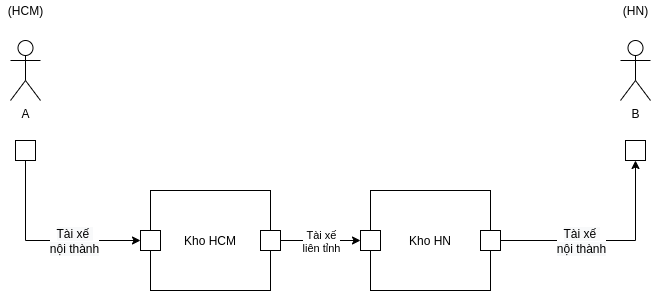
\includegraphics[width=1\textwidth]{/Summary.png}
		\centering
		\linebreak
		\caption{Luồng cơ bản giao nhận hàng hóa}
	\end{figure}
	\newpage
	
	
	\newpage
	\chapter{Công nghệ sử dụng}\label{chap:Tech}
		Trong quá trình làm luận văn, khi tìm hướng giải quyết cho từng bài toán, nhóm đã
		nghiên cứu và tìm tòi ra được những nguyên lý đằng sau cũng như những công nghệ giúp
		nhóm giải quyết được những khúc mắc gặp phải. Từ phía người dùng cho đến máy chủ
		. Sau đây, nhóm xin trình
		bày về các cơ sở lý thuyết và công nghệ chính mà nhóm sẽ sử dụng.
		
	\section{Front-end}
	\subsection{SPA}
		 Web sẽ thiết kế theo kiểu Single Page Application (SPA) thay vì theo kiểu truyền thống là Server side rendering. Ưu điểm của cách thiết kế này là web sẽ có trải nghiệm như khi dùng ứng dụng trên điện thoại hoặc máy tính. Mỗi lần thực hiện một thao tác hay chuyển trang trên web thì trình duyệt sẽ không phải load lại trang nữa. Việc này được thực hiện bằng cách sử dụng AJAX để lấy dữ liệu một cách bất đồng bộ từ phía server mỗi khi có một event do người dùng thực hiện trên trình duyệt. Sau đó, ta sẽ sử dụng dữ liệu lấy được (Thường là dưới dạng JSON) để đổ giao diện lên trình duyệt hiển thị cho người dùng.
		 
		 \begin{figure}[H]
		 	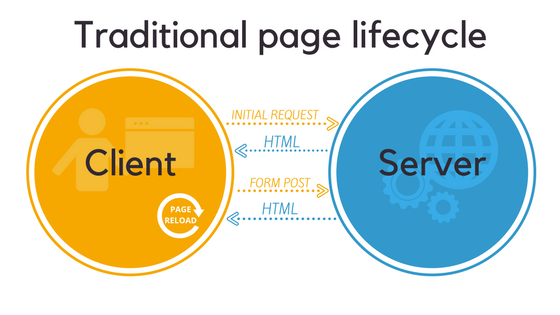
\includegraphics[width=0.8\textwidth]{/MPA.png}
		 	\centering
		 	\linebreak
		 	\caption{Luồng dữ liệu của các trang web MPA truyền thống}
		 \end{figure}
		 
		 \begin{figure}[H]
		 	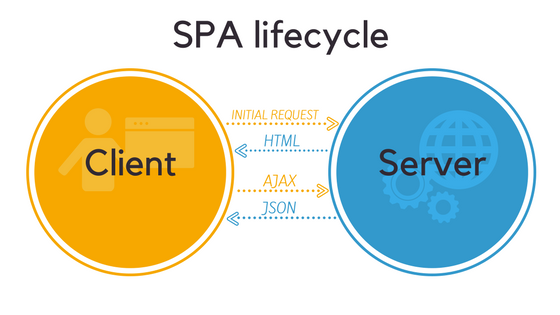
\includegraphics[width=0.8\textwidth]{/SPA.png}
		 	\centering
		 	\linebreak
		 	\caption{Luồng dữ liệu của các trang web SPA}
		 \end{figure}
    
	\subsection{ReactJS}
		\textbf{ReacJS} được phát triển bởi Facebook là một thư viện rất phổ biến để phát triển các ứng dụng web SPA hiện nay. React Cho phép người lập trình có thể chia ứng dụng thành các component và tái sử dụng, nhờ vậy mà tiết kiệm được thời gian lập trình. Hơn nữa, cơ chế DOM ảo \textbf{(Virtual DOM)} mới chính là điểm đặc biệt hơn cả của thư viện ReactJS. Cập nhật cây DOM là một tác vụ khá tốn chi phí. Nếu như để lập trình một cách thông thường, lập trình viên tự quản lí DOM bằng các Native API của môi trường web thì sẽ dễ gây ra vấn đề về hiệu suất. Chính vì vậy ReactJS sẽ giúp ta cập nhật DOM bằng cách quản lí ngầm một cây DOM ảo và sẽ đối chiếu những thay đổi so với các phiên bản DOM ảo trước đó để cập nhật lên cây DOM thật, giúp ứng dụng web tăng hiệu suất. Chính vì những lí do trên mà nhóm quyết định sẽ sử dụng thư viện này để phát triển luận văn này.\\
		
		\begin{figure}[H]
			
\includegraphics[width=0.8\textwidth]{/ReactJS.jpg}
			\centering
			\linebreak
			\caption{ReactJS và những lợi ích khi sử dụng}
		\end{figure}
		
		Bên cạnh đó, ReactJS cho phép người lập trình có thể viết bằng 2 ngôn ngữ: Javascript và Typescript. Javascript đã ra đời và được sử dụng từ rất lâu. Hiện nay, đây là ngôn ngữ được rất nhiều lập trình viên sử dụng, cả trong việc phát triển ứng dụng phía client-side lẫn phía server-side. JS là một ngôn ngữ prototype-based hỗ trợ cả lập trình hướng đối tượng và lập trình hàm, các tính năng được bảo trì và phát triển liên tục. Tuy vậy, quá linh động cũng là một điểm yếu của ngôn ngữ này. JS không kiểm tra ràng buộc kiểu khi chúng ta viết mã nguồn. Người lập trình có thể sử dụng một biến mà không cần khai báo kiểu, khiến cho việc truyền tham số hay khi tương tác các biến khác kiểu trở nên khó kiểm soát. Lấy ví dụ đơn giản như biểu thức "1" + 1 sẽ là hợp lệ và không bị bắt lỗi trong quá trình kiểm tra kiểu tĩnh khi chúng ta lập trình. Hay khi ta định nghĩa một hàm với các tham số cần truyền vào, do JS không hỗ trợ khai báo kiểu nên khi gọi hàm ta có thể truyền bất cứ tham số với bất cứ kiểu nào, làm cho hàm có thể thực thi ngoài ý muốn. Chính vì vậy, TypeScript ra đời để giải quyết vấn đề của JS kể trên. TypeScript yêu cầu người dùng định nghĩa kiểu rõ ràng cho các biến, kiểu trả về của hàm và bắt lỗi các biểu thức mà có sự tương tác của các biến không tương thích kiểu. Nhờ vậy, Sử dụng TS sẽ giúp cho mã nguồn của dự án dễ đọc, minh bạch, dễ bảo trì và phát triển hơn rất nhiều.
		
		\begin{figure}[H]
			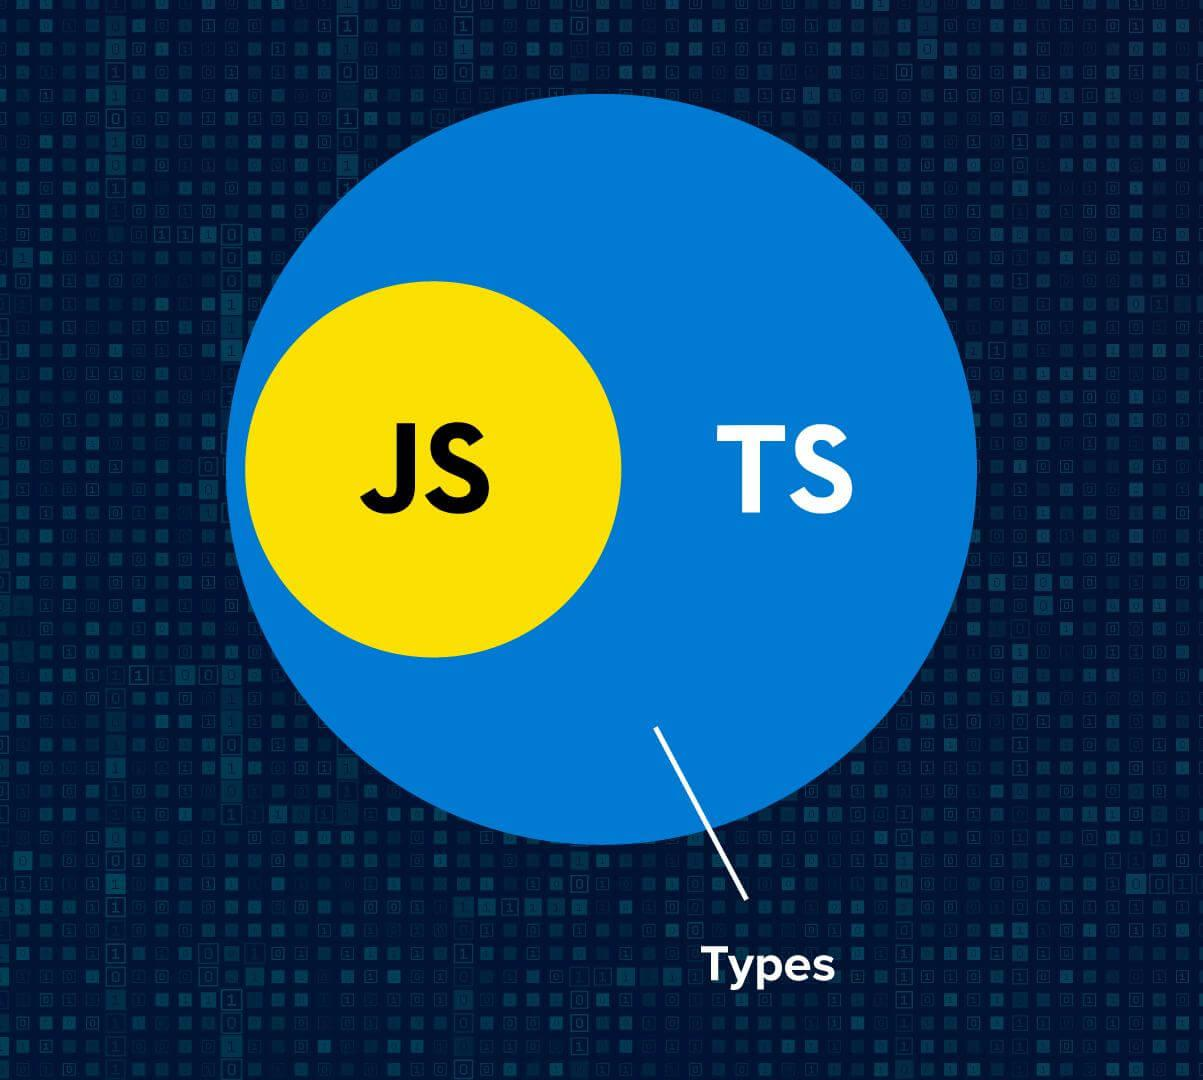
\includegraphics[width=0.8\textwidth]{/TypeScript.jpg}
			\centering
			\linebreak
			\caption{TypeScript là phiên bản mở rộng của JS có hỗ trợ kiểm tra kiểu tĩnh}
		\end{figure}
	
        \subsection{Continuous integration / Continuous deployment (CI/CD)}	
		Do web SPA sẽ trả về file html tĩnh cho người dùng tương tác (Dữ liệu hiển thị được cập nhật bằng cách tương tác với API phía server) nên ta có thể host website trên những dịch vụ cho host static web miễn phí. Nhóm sẽ chọn dịch vụ host web tĩnh miễn phí của gitlab để làm môi trường test (staging). Ưu điểm của gitlab là vừa có thể giúp nhóm quản lí source code cũng như cung cấp dịch vụ Continuous integration (CI) và continuous delivery (CD) giúp có thể deploy ứng dụng một cách tự động mỗi khi ta push code lên gitlab.\\
		
		Cụ thể, CI/CD giúp chúng ta chỉ phải code, chia branch đẩy lên git. Các công đoạn như unit test, deployment sẽ được gitlab-runner thực hiện một cách tự động mỗi khi có thay đổi mã nguồn. Bất kì ứng dụng được phát triển hiện nay đều cần phải qua khâu Unit Test do chính người lập trình viết trước khi được chuyển qua cho bộ phận kiểm thử phần mềm. Khi ta đẩy mã nguồn lên git mà quên chạy lệnh để kiểm thử unit test ở dưới máy local thì gitlab-runner sẽ giúp nhóm lập trình chạy các test case đó và sẽ thông báo trên giao diện git nếu có test case bị fail. Sau giai đoạn chạy các unit test và đã qua hết các test case thì tất nhiên, ứng dụng phải được deploy lên các môi trường (staging, production, etc). Việc phải SSH vào server host ứng dụng, sau đó tải mã nguồn mới nhất về, build ứng dụng ra các file tối ưu để chạy là khá tốn thời gian. Các thao tác trên thực chất cũng chỉ là chạy các câu lệnh trên terminal, vậy tại sao không để hệ thống tự động chạy những câu lệnh đó? Ta chỉ cần liệt kê các câu lệnh của một hành động cần phải thực hiện theo đúng thứ tự và hệ thống CI/CD của gitlab sẽ tự động chạy các câu lệnh đó cho chúng ta.
		
		\begin{figure}[H]
1			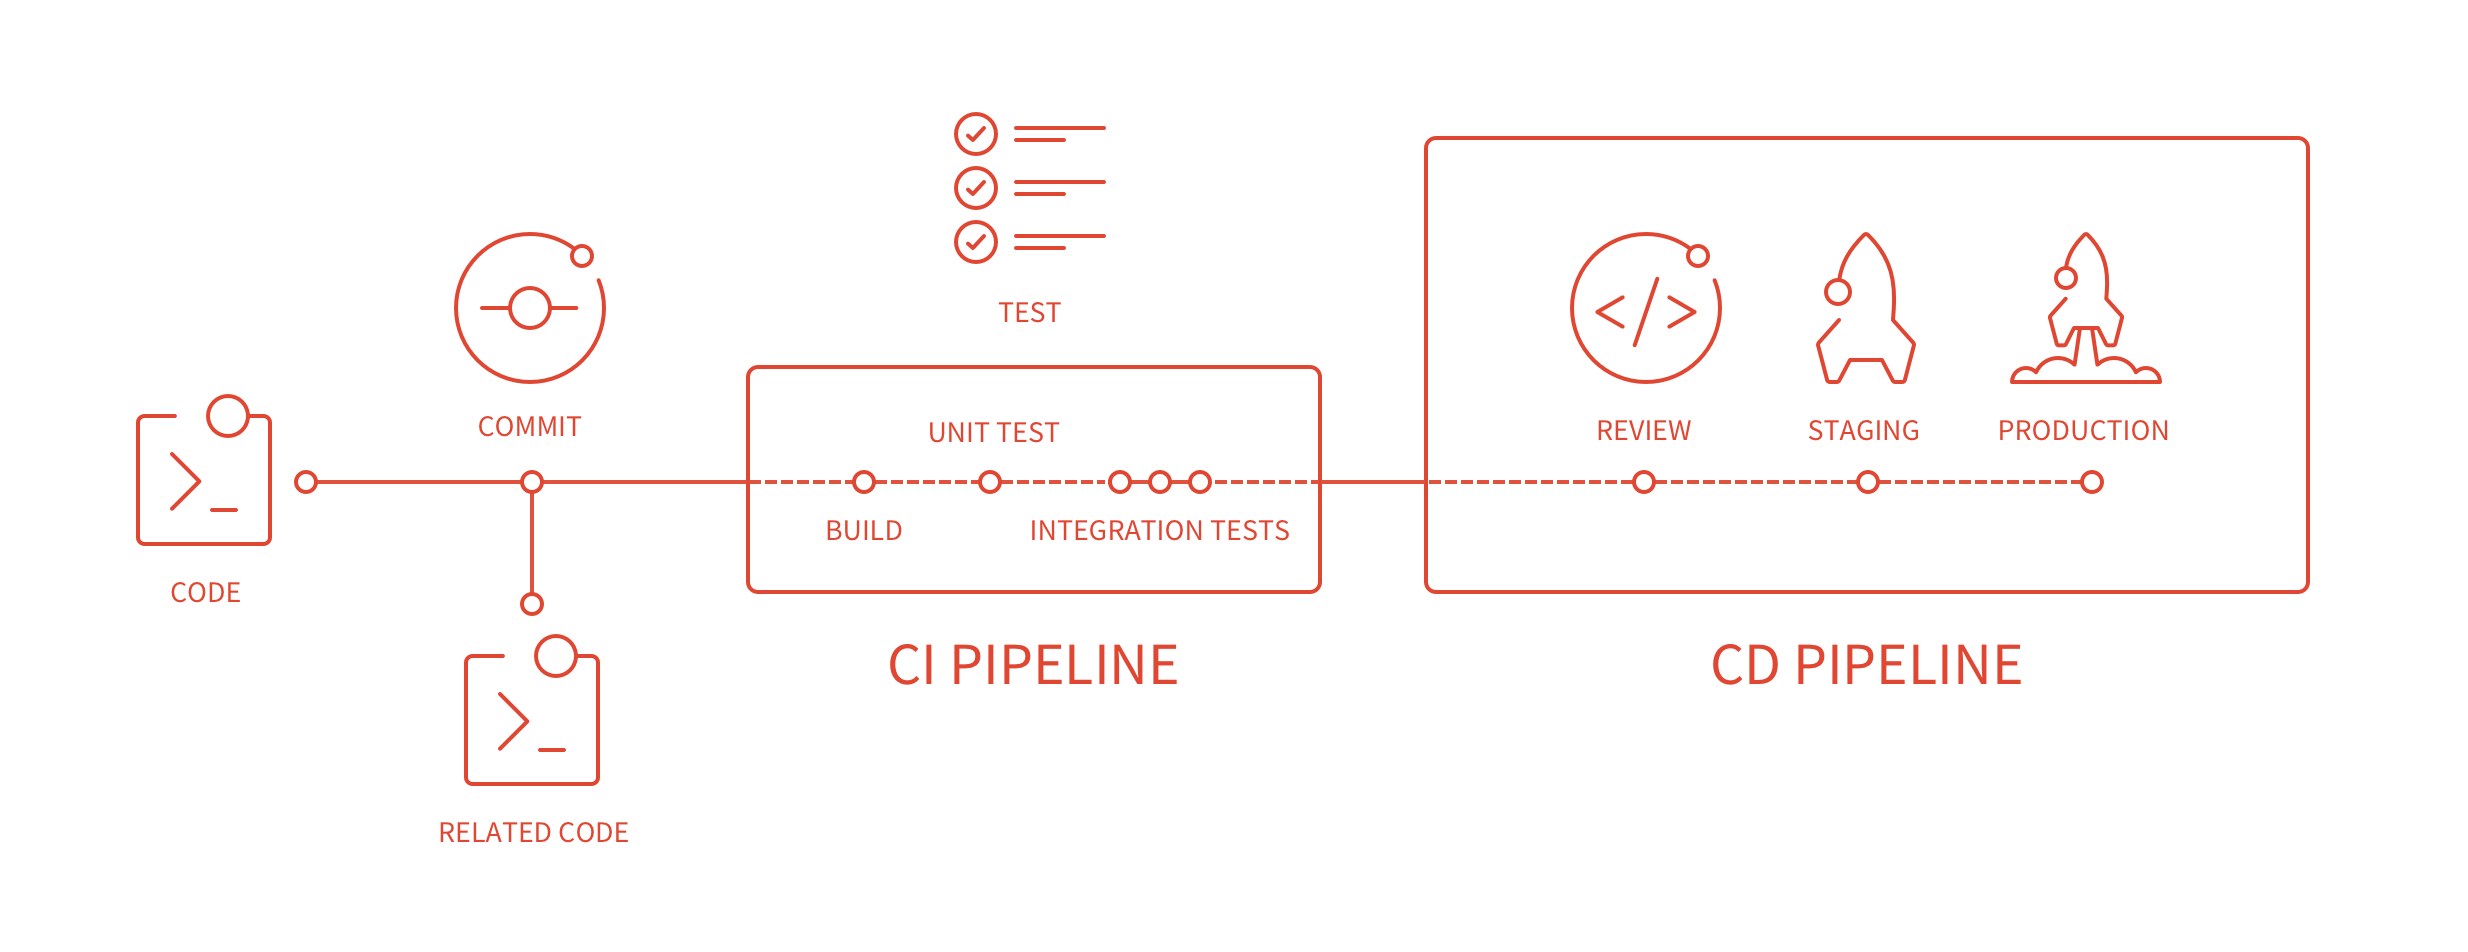
\includegraphics[width=1\textwidth]{/cicd.png}
			\centering
			\linebreak
			\caption{Gitlab CICD}
		\end{figure}
	
		\subsection{Những thư viện nổi bật giúp hiện thực chức năng hệ thống}
			Một số lập trình viên rất thích việc xây dựng mọi thứ từ đầu và hạn chế sử dụng thư viện càng nhiều càng tốt. Tuy vậy, có những tính năng đã được một số thư viện hỗ trợ đầy đủ và đã được kiểm thử qua hàng ngàn người dùng. Khi đó, ta nên sử dụng thư viện để tiết kiệm thời gian phát triển cũng như có thể sử dụng ngay lập tức tính năng chất lượng đã qua kiểm thử. Nhóm sẽ liệt kê một số thư viện nổi bật (Ngoài thư viện chính React) mà nhóm đã dùng để hiện thực một vài chức năng của hệ thống: \\
			
			Nhóm sẽ giới thiệu một số thư viện được áp dụng trong việc viết code phía client mà nhóm thấy nổi bật để trình bày:
			
			\begin{itemize}
				\item \textbf{chart.js (version 2.9.4):} Dùng để hiện thực chức năng tạo biểu đồ thống kê của admin.
				\item \textbf{date-fns (version 2.21.1):} Dùng để thực hiện việc tính toán ngày tháng như lấy thời gian bắt đầu / kết thúc của ngày, tăng giảm số ngày vv...
				\item \textbf{antd (version 4.9.4):} Thư viện CSS và component tương thích với React.
				\item \textbf{json-bigint (version 1.0.0):} Giúp parse ra được ID lớn của đơn hàng thành chuỗi dạng string.
				\item \textbf{@react-pdf/renderer (version 2.0.8):} Giúp tạo ra template cho phiếu nhập/xuất kho dưới dạng pdf.
				\item \textbf{gzipper (version 4.5.0):} Giúp tạo ra những file gzip của những file static đã build ra. Như vậy sẽ giảm dung lượng đường truyền mạng cần thiết để tải file và trang web sẽ hiển thị nhanh hơn vào lần đầu tiên truy cập.
			\end{itemize}
			
	
		\subsection{Giám sát lỗi hệ thống bằng dịch vụ Sentry}
			\subsubsection{Giới thiệu về Sentry}
				Một hệ thống không những phải hoạt động tốt mà còn cần phải có hệ thống ghi log và báo cáo lỗi không mong muốn xảy ra từ người dùng. Thay vì phải tự hiện thực lại hệ thống như trên thì nhóm đã quyết định sử dụng một dịch vụ trực tuyến khá phổ biến và nổi tiếng hiện nay: Sentry. Về cơ bản. Sentry giúp chúng ta theo dõi lại những lỗi xảy ra bên trong ứng dụng trong quá trình người dùng sử dụng. Thông thường khi lỗi xảy ra, người dùng sẽ có xu hướng tắt ứng dụng và mở lại chứ không report lại cho bên phía đội ngũ phát triển. Sentry sẽ tự động gửi report chi tiết về lỗi đó một cách tự động và nhanh chóng. Giúp cho người lập trình có thể nhanh chóng cập nhật bản vá sửa lỗi đó trước khi nhiều người dùng bị lỗi tương tự.
				
			\subsubsection{Áp dụng sentry cho hệ thống giao hàng liên tỉnh}
			 	Nhận thấy tác dụng hữu ích và đồng thời muốn học thêm những công nghệ đang thịnh hành ngoài thị trường. Nhóm chúng em đã thử áp dụng Sentry vào hệ thống giao hàng liên tỉnh này. Sau đây là một số kết quả mà nhóm đã thu được từ việc áp dụng Sentry:
			 	
			 	\begin{figure}[H]
			 		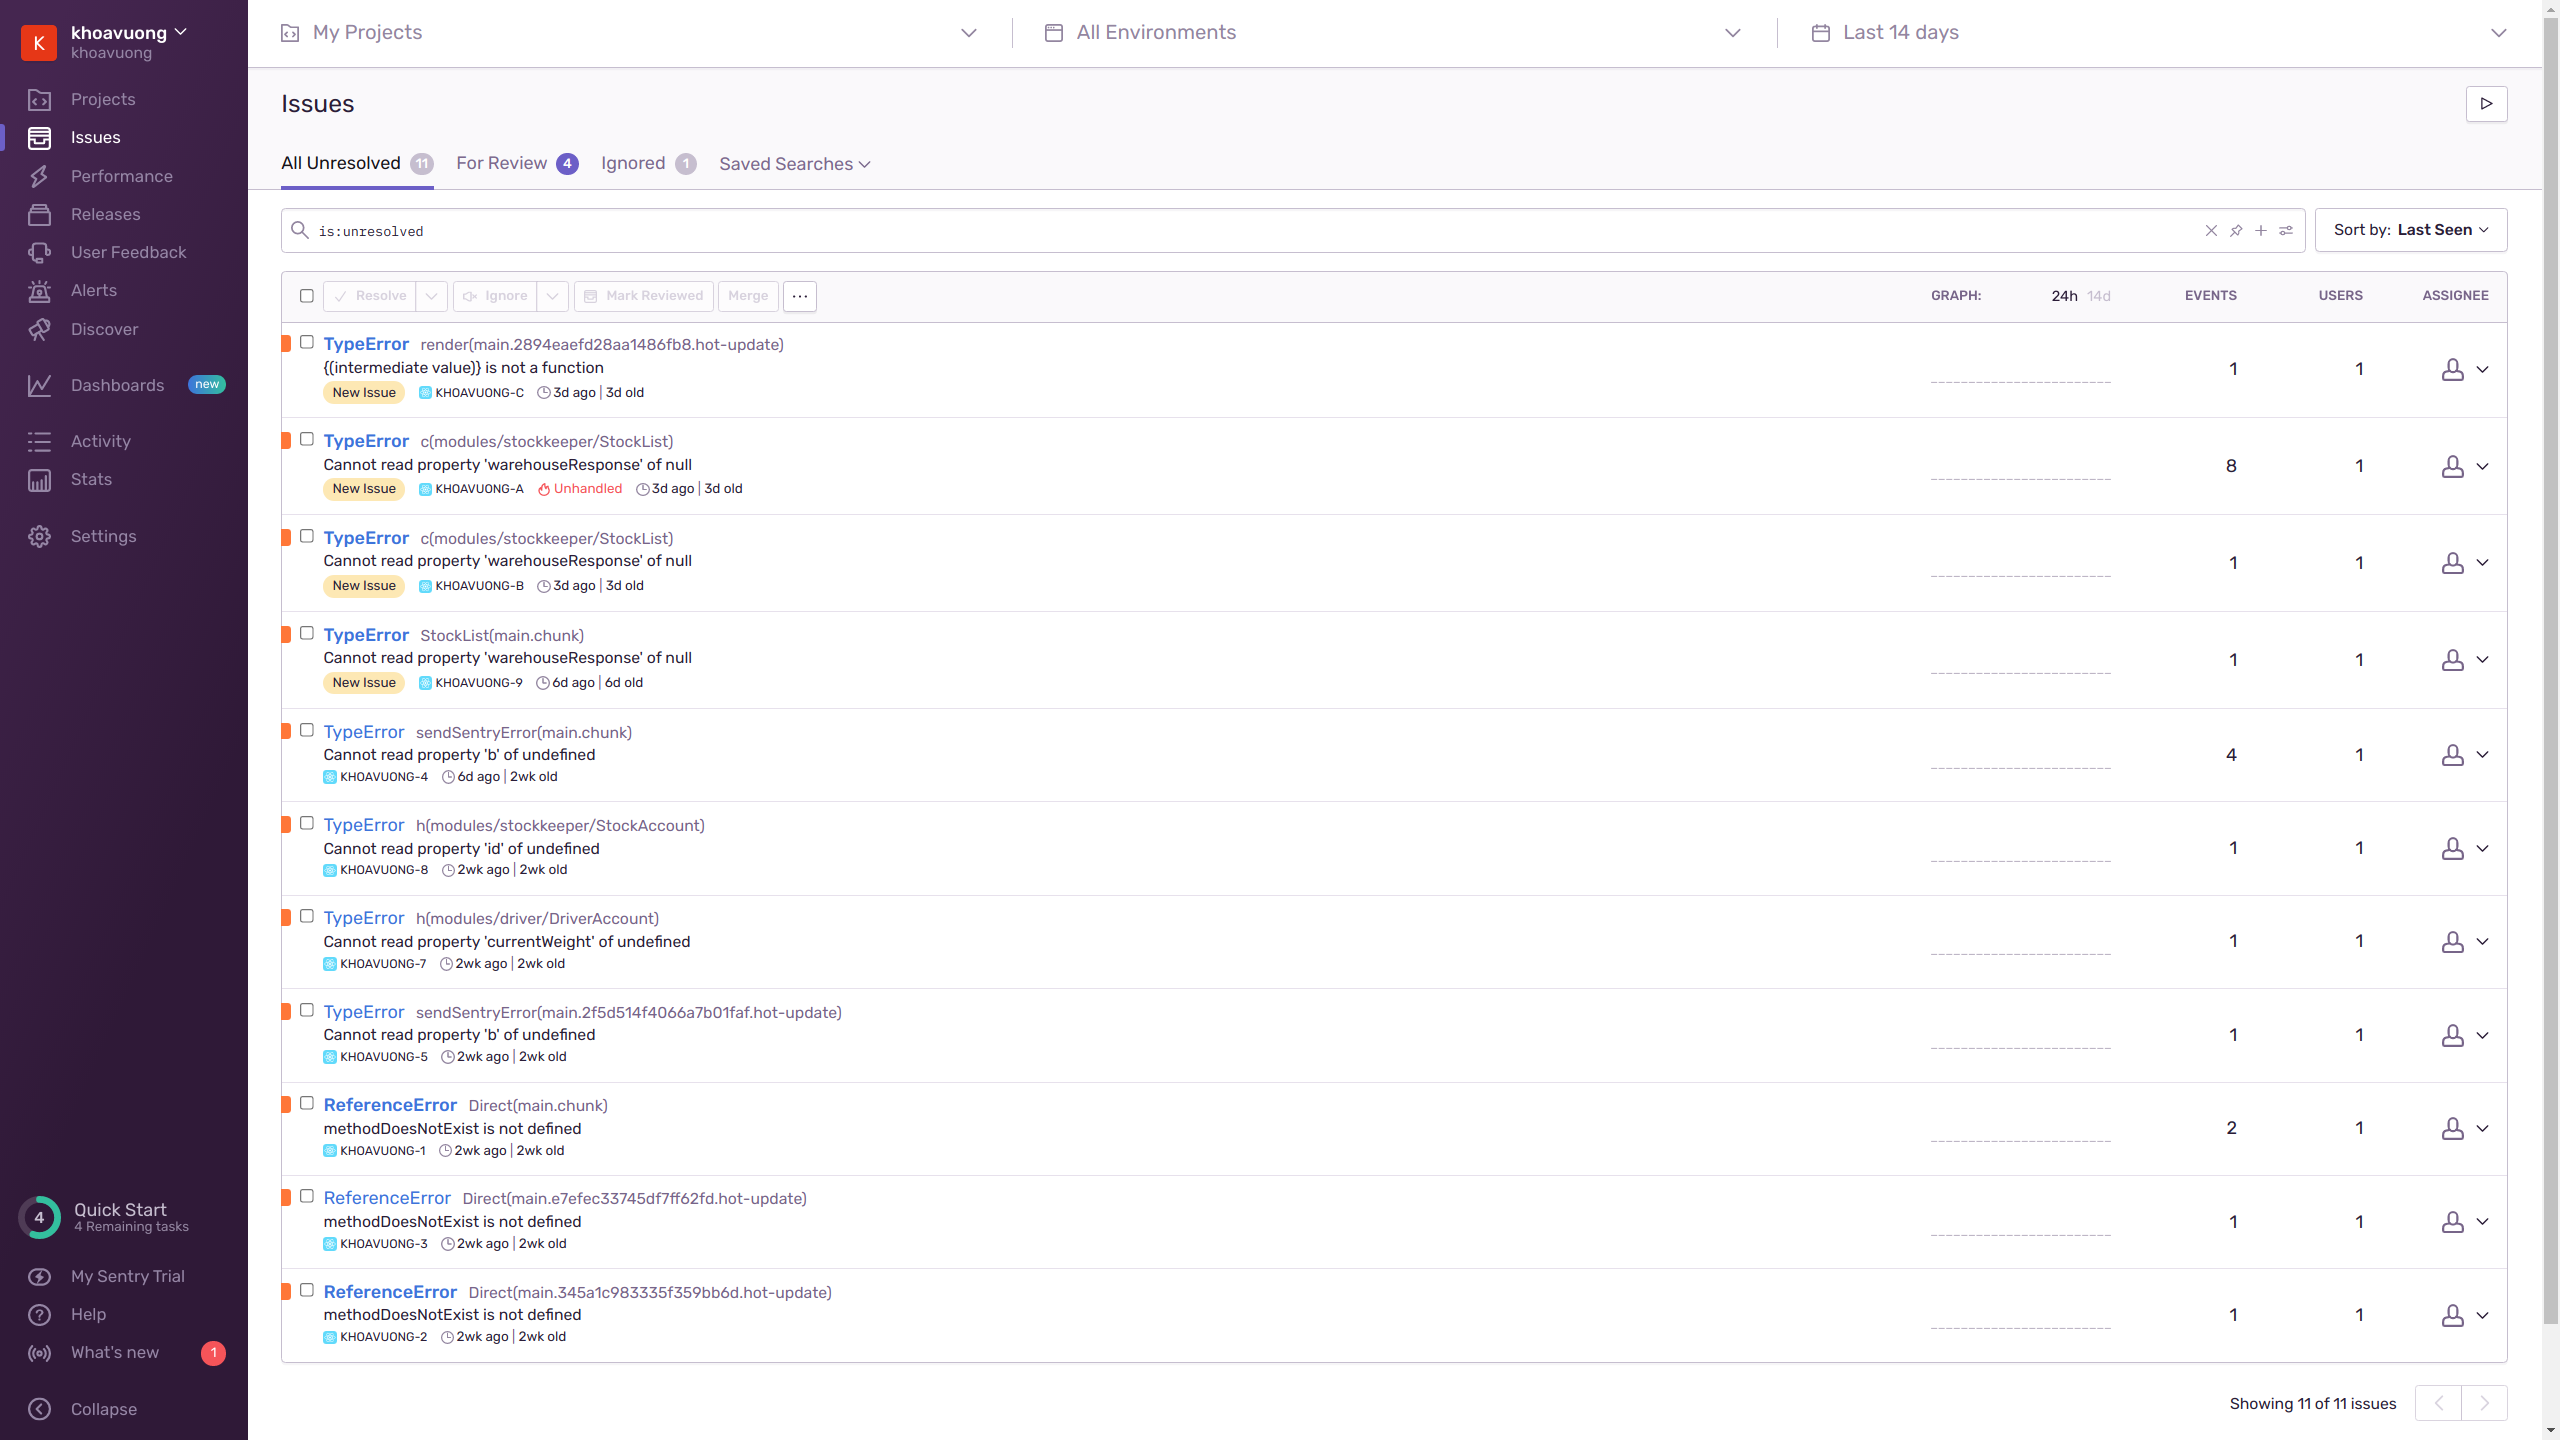
\includegraphics[width=0.8\textwidth]{/sentry/sentry_dashboard.png}
			 		\centering
			 		\caption{Giao diện dashboard để xem những lỗi được gửi về}
			 	\end{figure}
		 	
		 		Có thể thấy giao diện trên liệt kê ra những lỗi chưa được xử lý của ứng dụng khi người dùng tương tác. Ở giao diện dashboard đó ta có thể chọn một hoặc nhiều lỗi được gửi về và đánh dấu đã xử lí (Resolve) sau khi đã thực hiện bản vá sửa lỗi hoặc bỏ qua (Ignore) nếu như lỗi đó không cần phải giải quyết. Những lỗi đã được xử lí sẽ bị mất đi trong danh sách lỗi ở màn hình dashboard đó. \\
		 		
		 		Ngoài ra, khi click vào liên kết của một lỗi cụ thể. Sentry sẽ đưa ta đến một giao diện để xem một cách chi tiết thông tin về lỗi đó:
		 		
			 	\begin{figure}[H]
			 		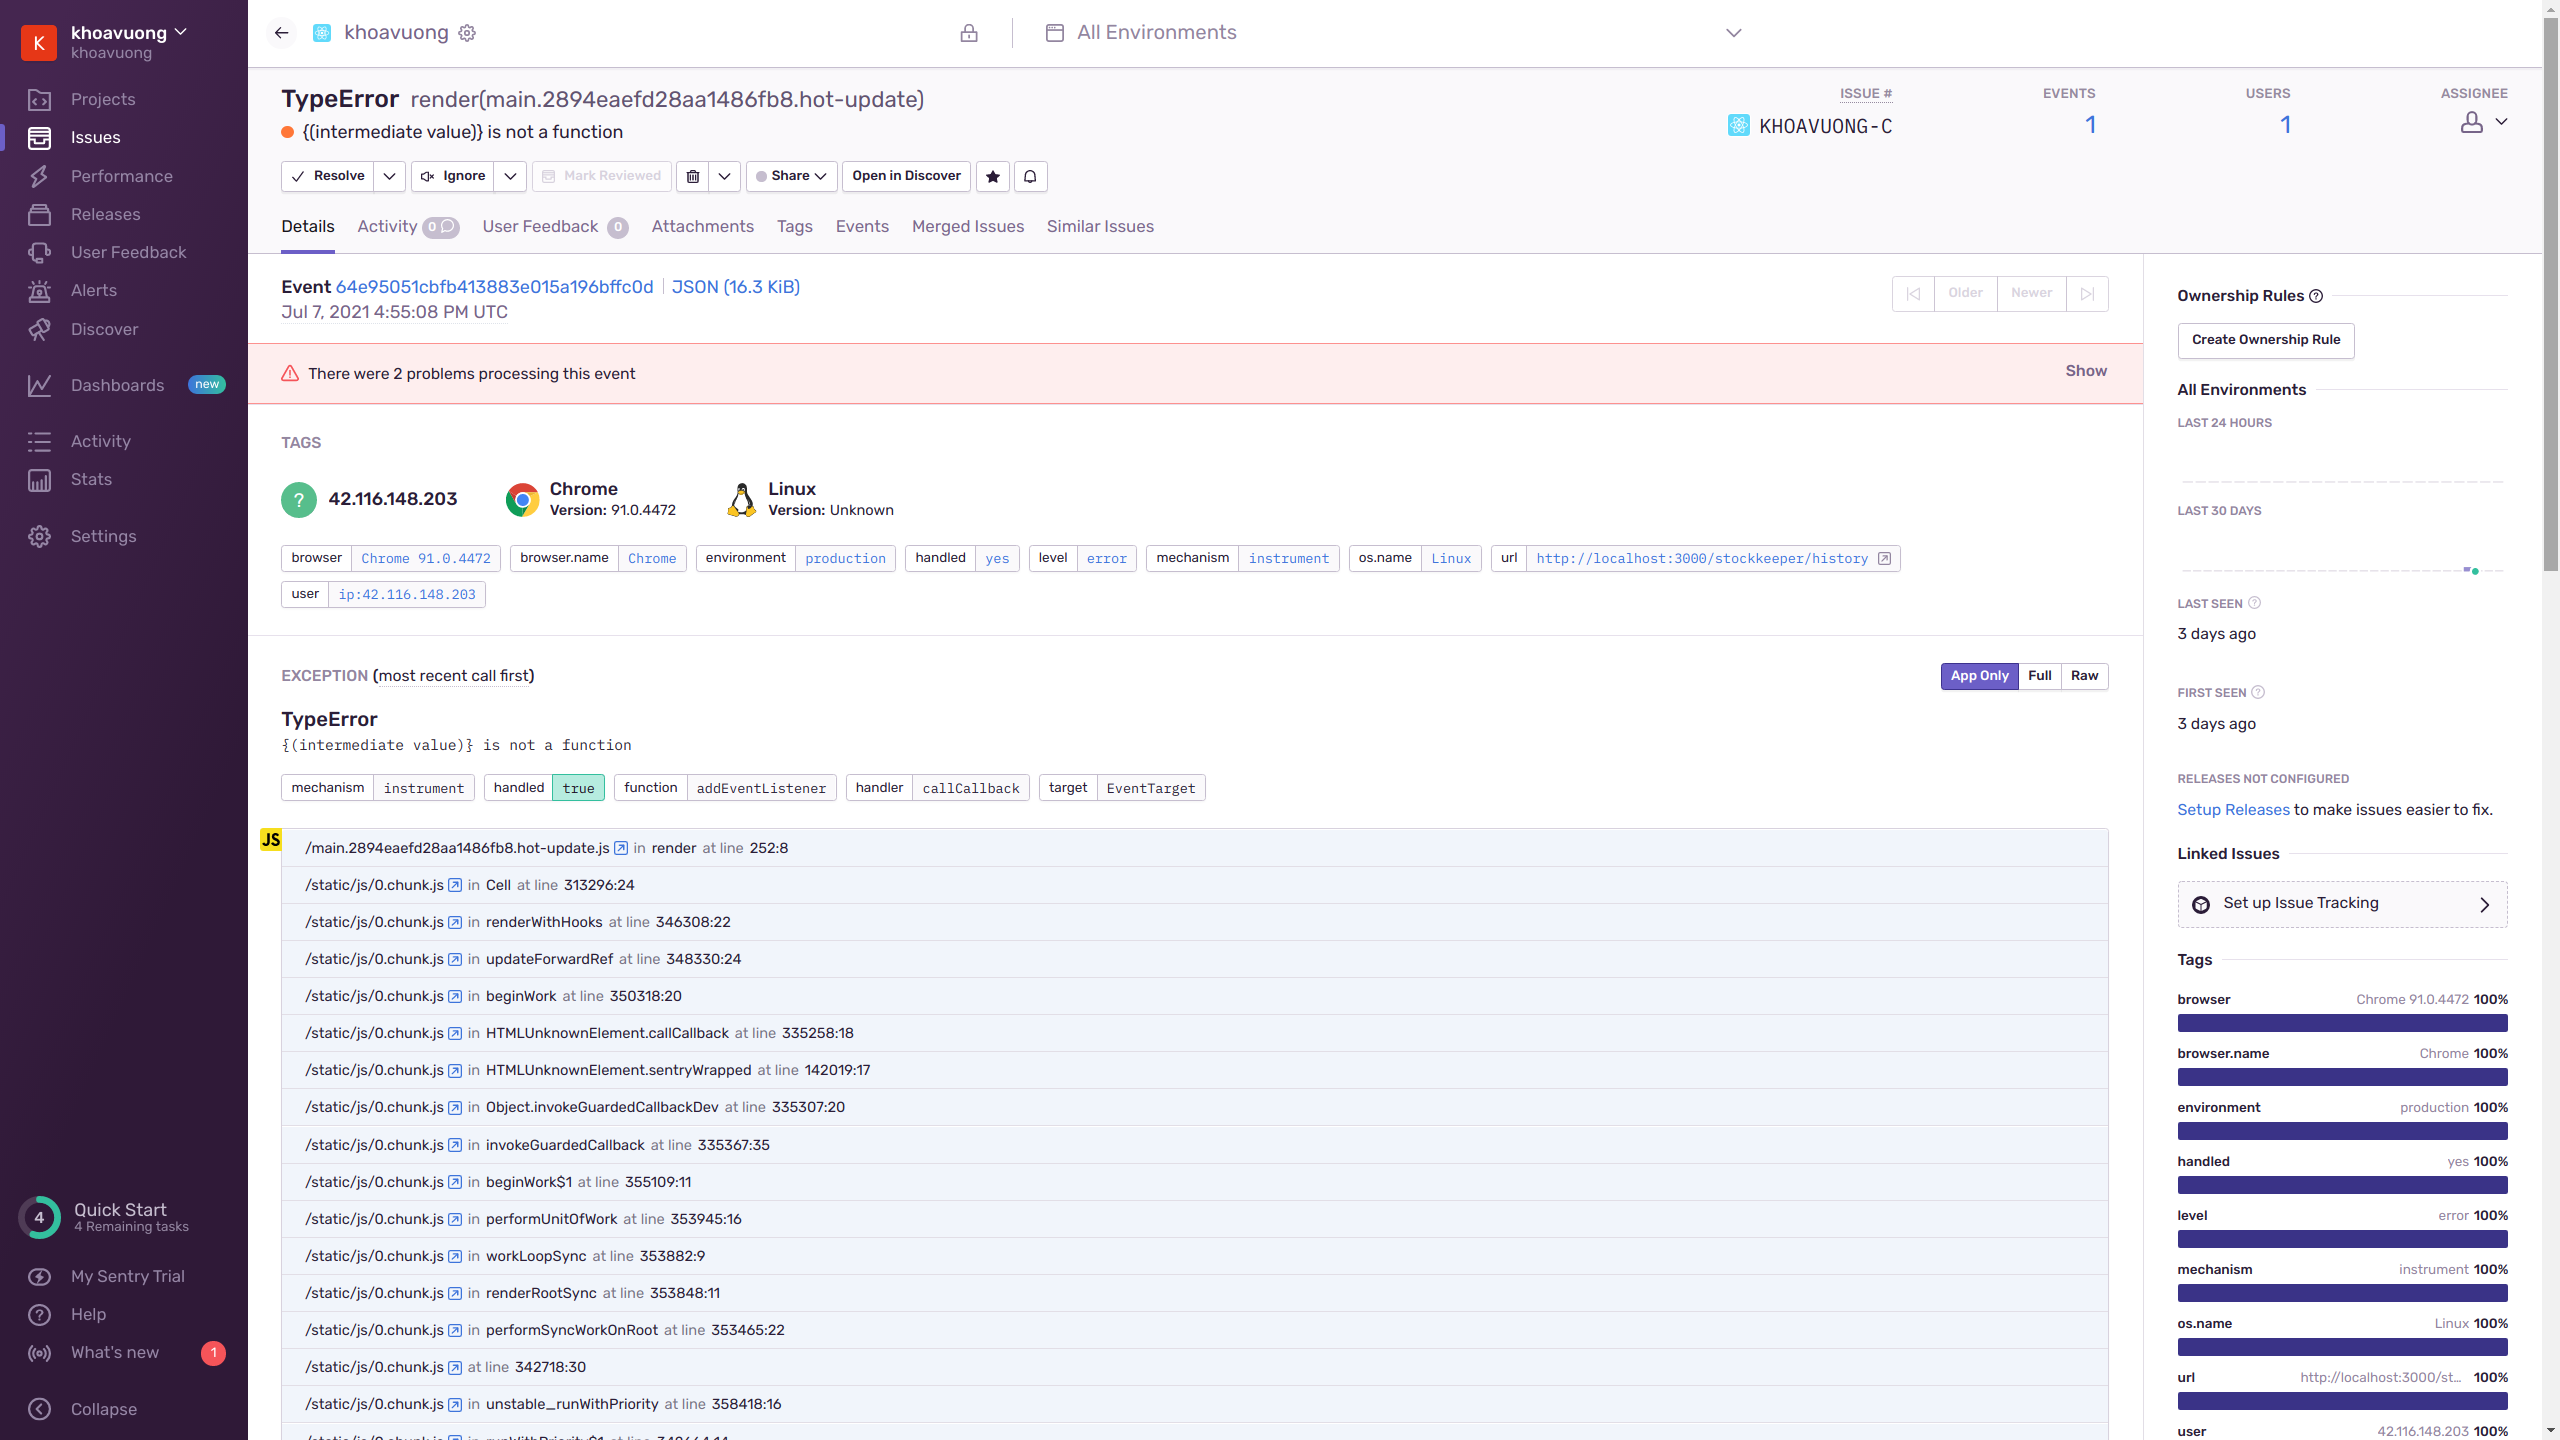
\includegraphics[width=0.8\textwidth]{/sentry/sentry_detail_1.png}
			 		\centering
			 		\caption{Giao diện xem lỗi gửi về chi tiết (Nửa trên màn hình)}
			 	\end{figure}
		 	
		 		\begin{figure}[H]
		 			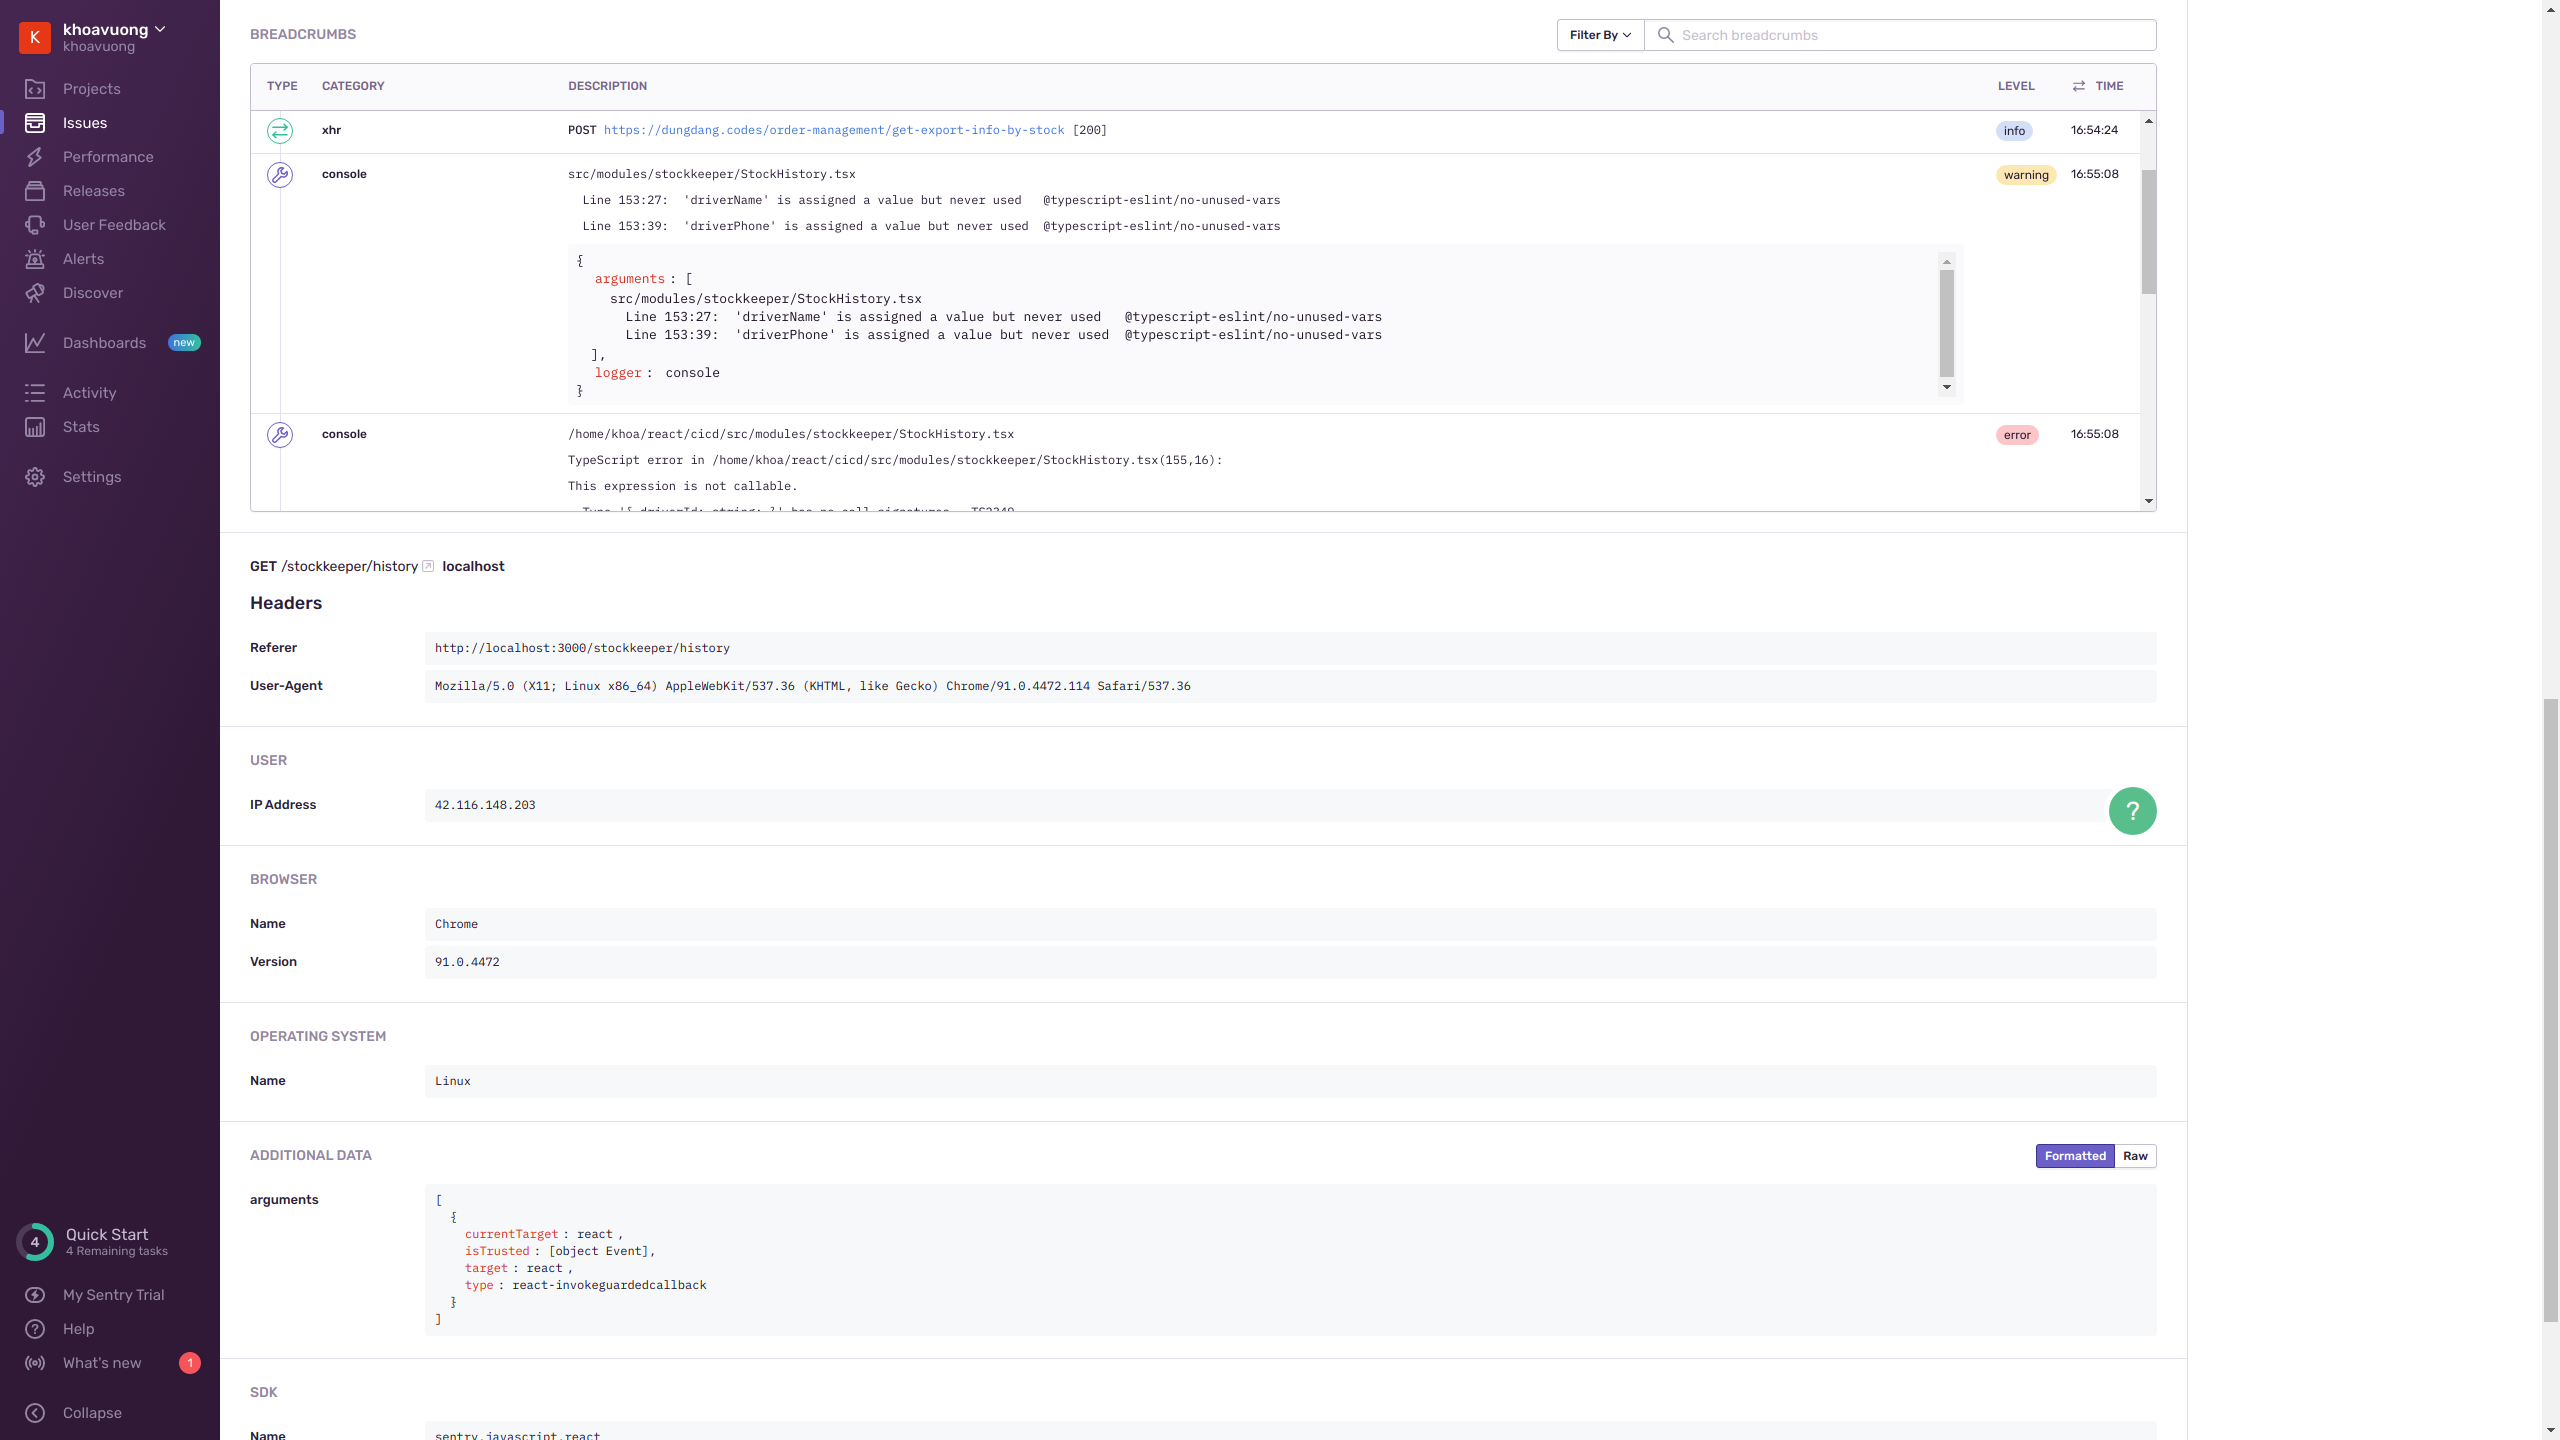
\includegraphics[width=0.8\textwidth]{/sentry/sentry_detail_2.png}
		 			\centering
		 			\caption{Giao diện xem lỗi gửi về chi tiết (Nửa dưới màn hình)}
		 		\end{figure}
			 	
			 	Giao diện đó cung cấp cho người lập trình toàn bộ thông tin quan trọng để có thể bắt đầu việc debug và sửa lỗi. Có thể kể đến một số thông tin hữu ích như ngày xảy ra lỗi, trình duyệt web, địa chỉ IP, OS của người dùng. Không những thế, Sentry còn liệt kê cho ta chi tiết lỗi xảy ra ở đoạn mã lệnh nào giúp cho người lập trình dễ dàng phát hiện đoạn mã lỗi để sửa. Ở ví dụ cụ thể trong hình trên. Ta có thể thấy được lỗi xảy ra tại địa chỉ IP 42.116.148.203, trình duyệt web Chrome và hệ điều hành Linux. Đoạn lệnh lỗi cũng được chỉ ra nằm ở tập tin nào và nguyên nhân xảy ra lỗi. \\
			 	
			 	Tóm tắt lại, Sentry là một nền tảng rất phổ biến hiện nay giúp cho hệ thống chúng ta xây dựng có thể nhanh chóng phát hiện lỗi từ phía người dùng. Hầu như mọi dự án lớn đều đang sử dụng Sentry và hiệu quả nó mang lại là không phải bàn cãi.
			 	
			 	\subsection{Phân tích số lượng và hành vi người dùng với Google Analytics}
			 	Một website không chỉ cần có hệ thống giám sát lỗi không mong muốn từ người dùng mà cũng cần phải có một hệ thống dùng để thống kê, theo dõi lưu lượng truy cập và những tương tác của người dùng với trang web. Từ đó đội ngũ phát triển có thể đưa ra những quyết định và những bản cập nhật để phục vụ nhu cầu người dùng tốt hơn. Cũng tương tự như trên, thay vì phải tốn thời gian và công sức xây dựng hệ thống đó thì nhóm cũng quyết định sử dụng một dịch vụ thống kê rất phổ biến và được ưa chuộng hiện nay: Google Analytics. Đây là một dịch vụ được cung cấp miễn phí bởi Google.
			 	
			 	\subsubsection{Áp dụng Google Analytics vào hệ thống}
			 	Nhận thấy đây là công nghệ rất phổ biến và hữu dụng. Nhóm đã quyết định sử dụng Google Analytics vào để có thể xem được chi tiết những thống kê người dùng truy cập đến trang web. Đây cũng là một cơ hội để học hỏi thêm một công nghệ mới được sử dụng bởi nhiều doanh nghiệp.\\
			 	
			 	Sau đây là một số tính năng theo dõi và thống kê thời gian thực của người dùng của website do Google Analytics đã thu thập:
			 	
			 	\begin{figure}[H]
			 		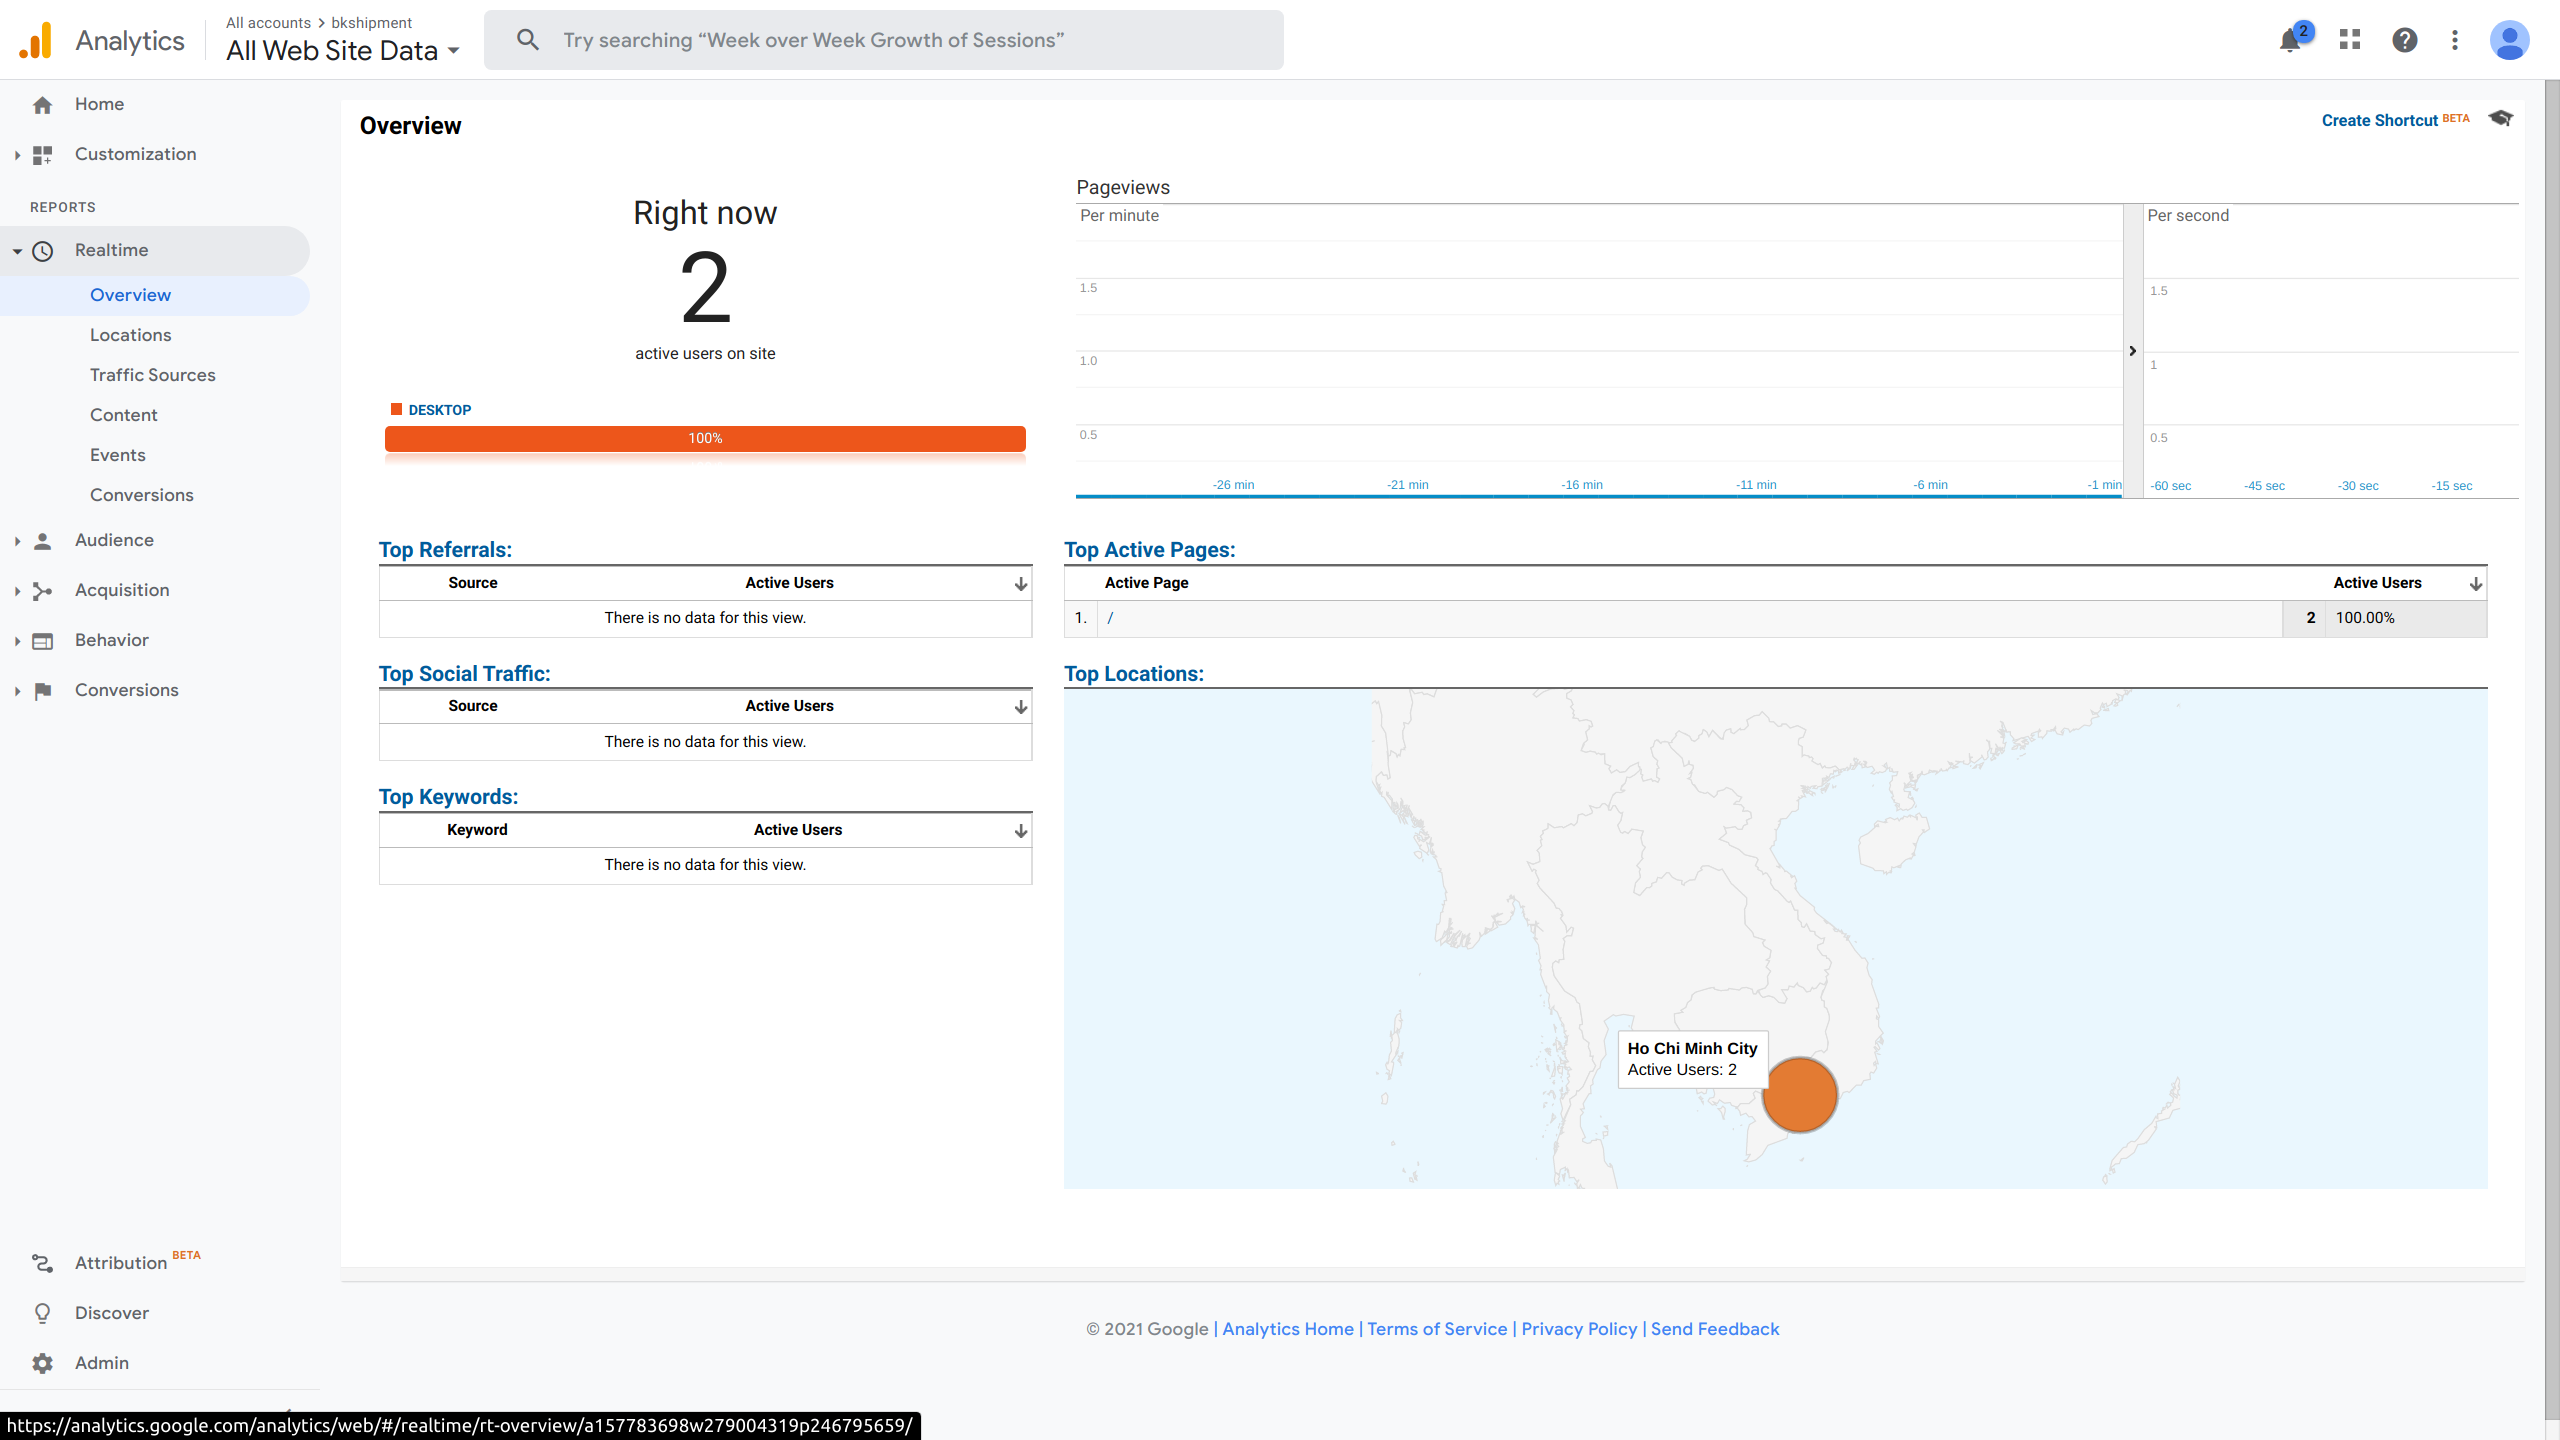
\includegraphics[width=0.8\textwidth]{/GA/GA_overview.png}
			 		\centering
			 		\caption{Màn hình thống kê thời gian thực tổng quan}
			 	\end{figure}
			 	
			 	\begin{figure}[H]
			 		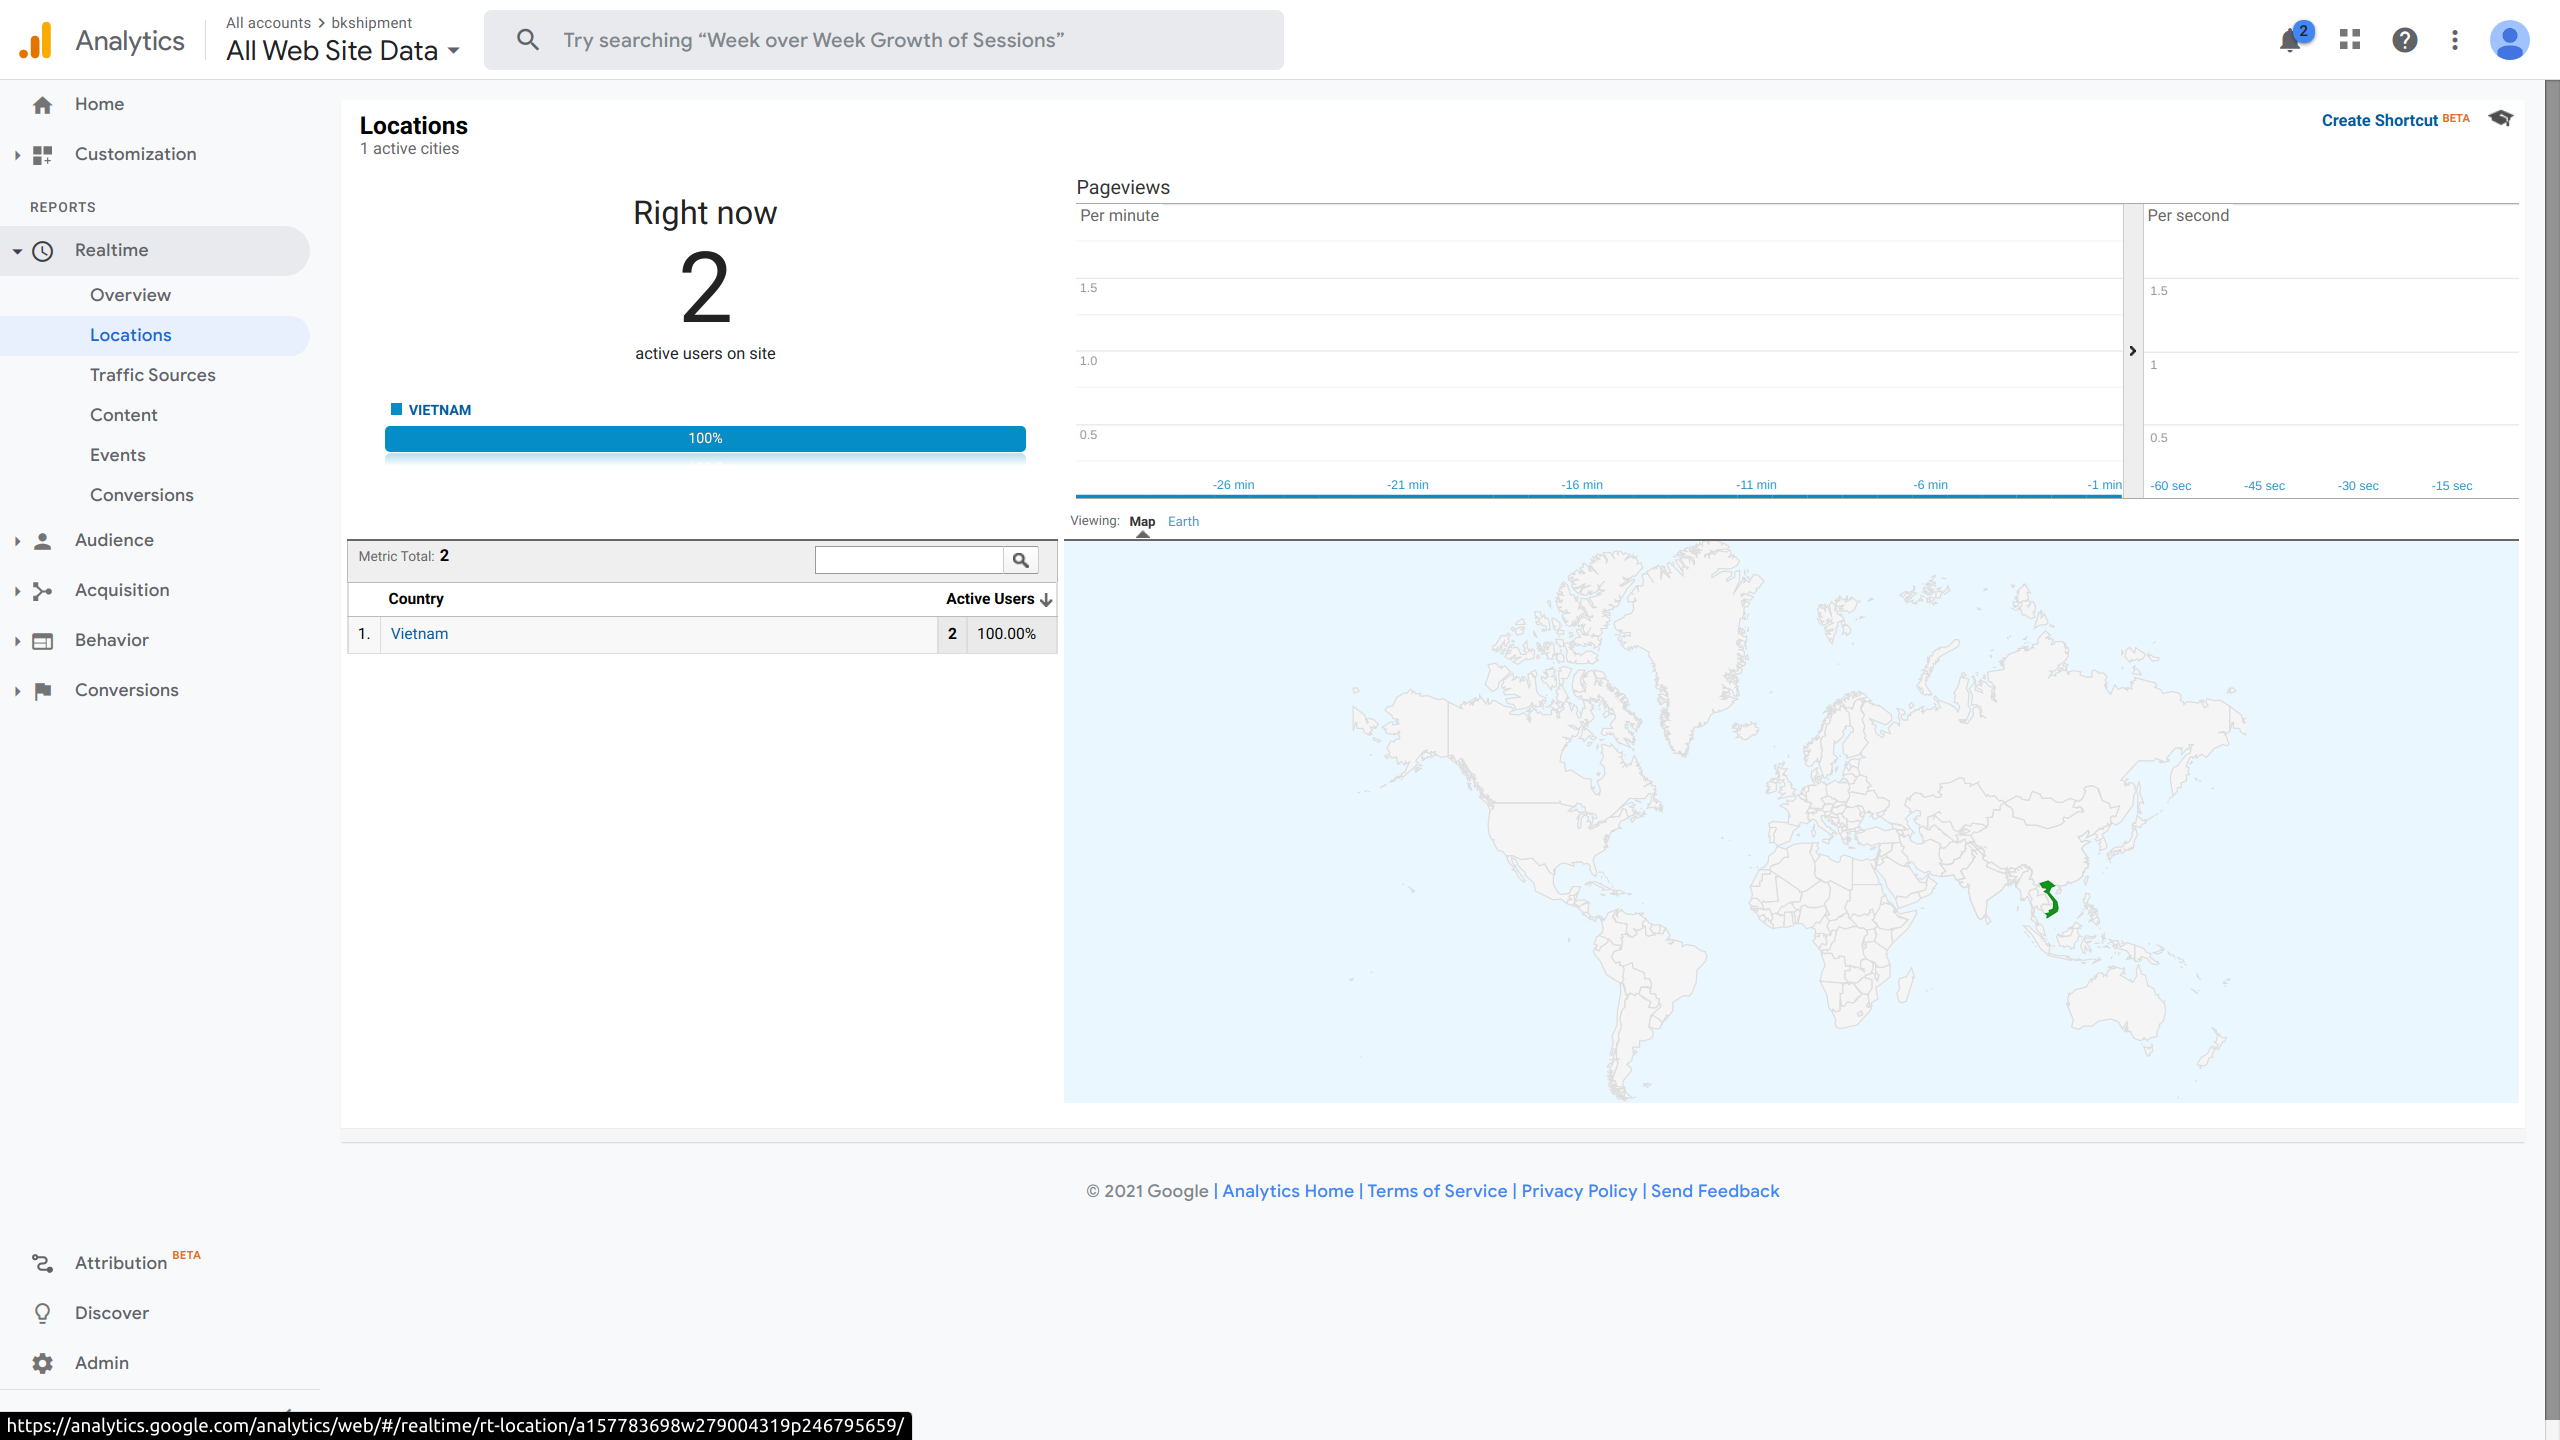
\includegraphics[width=0.8\textwidth]{/GA/GA_location.png}
			 		\centering
			 		\caption{Màn hình thống kê thời gian thực theo địa lý}
			 	\end{figure}
			 	
			 	\begin{figure}[H]
			 		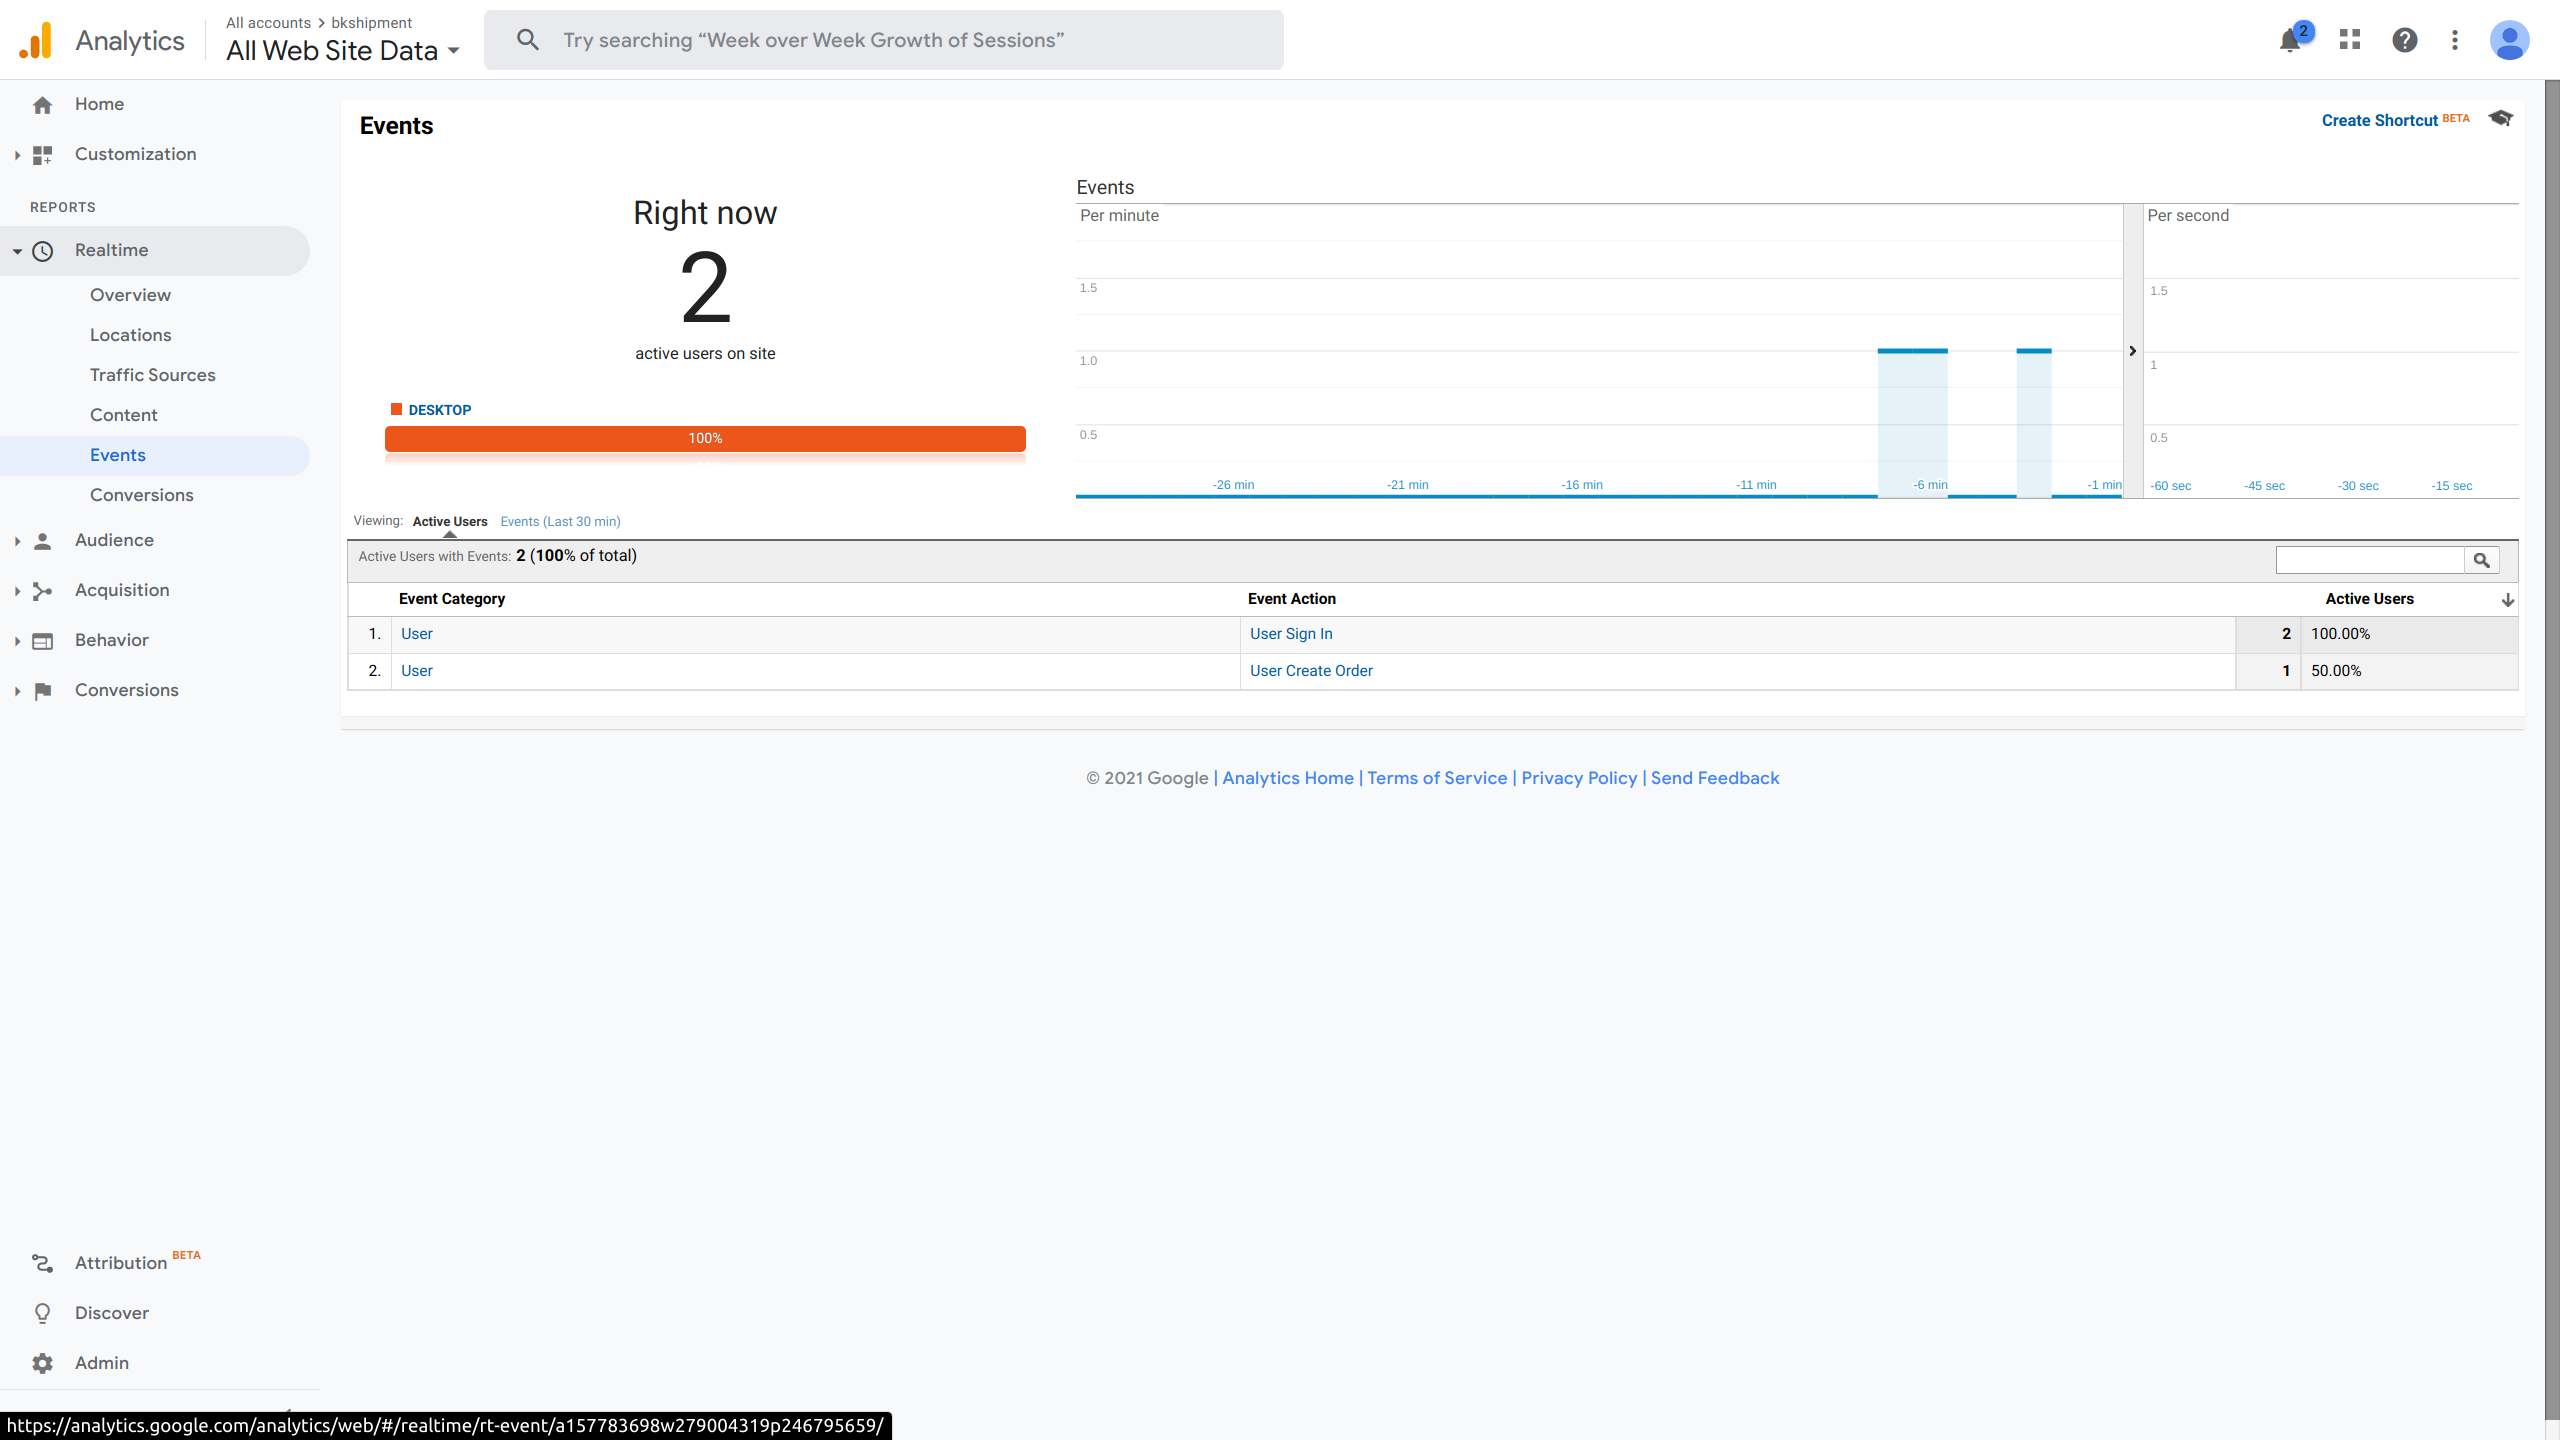
\includegraphics[width=0.8\textwidth]{/GA/GA_events.png}
			 		\centering
			 		\caption{Màn hình thống kê thời gian thực theo sự kiện}
			 	\end{figure}
			 	
			 	Ở các màn hình kể trên, ta đều có thể thấy số lượng người dùng đang truy cập website hiện tại (Ở ví dụ trong hình là 2). Google Analytics cũng giúp chúng ta thống kê người truy cập là ở những nước nào (Ví dụ trong hình là ở Việt Nam) và thống kê những tác vụ mà người dùng thực hiện (Ở ví dụ trong hình ta có thể thấy có 2 tác vụ là người dùng đăng nhập và người dùng tạo yêu cầu gửi hàng). Nhờ những thống kê trên mà đội ngũ phát triển hệ thống có thể đưa ra những quyết định phát triển cho tương lai phù hợp hơn.
			 	
			 	\subsection{Front-end Unit testing}
			 	Trong quá trình xây dựng phần mềm thì việc đảm bảo chất lượng và qui trình kiểm thử phần mềm cũng là một công đoạn rất quan trọng. Không có phần mềm nào là không có lỗi. Chính vì vậy, việc kiểm thử phần mềm giúp hạn chế tối đa lỗi trước khi đưa phần mềm cho khách hàng. Đương nhiên, ngoài đội ngũ xây dựng và phát triển phần mềm cũng cần một đội ngũ tester đảm bảo chất lượng sản phẩm. Tuy vậy, không có nghĩa là lập trình viên chỉ việc viết mã nguồn mà không phải thực hiện kiểm thử phần mềm. Lập trình viên ít nhất cũng nên viết kiểm thử đơn vị (Unit Test) để đảm bảo module mình viết ra ít lỗi nhất có thể và khi có sự thay đổi trong tương lai thì đảm bảo không gây lỗi cho các thành phần cũ của phần mềm.
			 	
			 	\subsubsection{Khái niệm về Unit Test}
			 	Unit Test là một loại kiểm thử phần mềm trong đó các đơn vị hay thành phần riêng lẻ của phần mềm được kiểm thử. Kiểm thử đơn vị được thực hiện trong quá trình phát triển ứng dụng. Mục tiêu của kiểm thử đơn vị là cô lập một phần code và xác minh tính chính xác của đơn vị đó.
			 	
			 	\subsubsection{Lợi ích và đánh đổi của Unit Test}
			 	Thông thường, ở một vài qui trình phát triển phần mềm, đội ngũ kiểm thử phần mềm sẽ yêu cầu lập trình viên phải thực hiện Sanity Test (Kiểm thử sơ bộ) để chắc chắn rằng những những chức năng chính của phần mềm hoạt động ổn định. Mỗi lần sanity test thường có từ vài chục cho đến vài trăm test case và những test case đó có thể xuất hiện lại sau mỗi bản cập nhật phần mềm. Việc phải kiểm đi kiểm lại những test case đó là điều cần thiết, tuy vậy nó khá tốn thời gian và nhàm chán. Chính vì vậy, nếu có thể viết unit test cho những test case đơn giản đó một cách tự động thì sẽ tiết kiệm được rất nhiều thời gian và đảm bảo tính chính xác nếu unit test của người lập trình viết ra có chất lượng tốt. Không những vậy, việc viết unit test sẽ giúp cho người lập trình cảm thấy tự tin hơn mỗi khi xây dựng một module mới hay chỉnh sửa module cũ. Nhờ vào những test case đã viết sẵn đó mà ta có thể chắc chắn sẽ không có lỗi liên quan xảy ra.\\
			 	
			 	Tuy rằng việc viết unit test có rất nhiều lợi ích nhưng có cũng những đánh đổi sau:
			 	\begin{itemize}
			 		\item Tốn thời gian và tương đối khó khăn. Viết test tuy giảm bớt thời gian và công sức cho giai đoạn duy trì (maintain) phần mềm nhưng sẽ làm mất thời gian lúc đầu để viết một unit test tốt.
			 		\item Test pass không có nghĩa ứng dụng, function của chúng ta chạy đúng hoàn toàn.
			 		\item Cũng đôi khi, test fail, nhưng ứng dụng, function vẫn chạy hoàn toàn bình thường. Việc viết test không tốt như vậy sẽ còn nguy hiểm hơn do nó tạo cho người lập trình một suy nghĩ rằng phần mềm viết ra không có lỗi, trong khi thực sự thì có.
			 	\end{itemize}
			 	
			 	\subsubsection{Viết unit test cho client-side code của hệ thống}
			 	Có thể hiểu nôm na, viết unit test cho Front-end thì ngoài viết test cho những hàm tính toán, ta còn có thể viết test để kiểm thử giao diện và hành vi khi một số sự kiện người dùng xảy ra. Chẳng hạn sau đây là một số thứ ta có thể kiểm thử ở client-side code:
			 	
			 	\begin{itemize}
			 		\item Kiểm thử xem một node trong cây DOM có xuất hiện (tồn tại) trong giao diện sau khi đã render component hay chưa. Chẳng hạn kiểm thử xem giao diện đăng nhập có tồn tại một nút với dòng chữ là "Đăng nhập" hay không. Hay nút đó có được áp dụng đúng class hay không để có style css đúng như mong muốn.
			 		\item Kiểm thử xem sau khi người dùng đã nhập đủ thông tin đăng nhập và ấn nút đăng nhập, người dùng có chuyển đến trang màn hình chính hay không.
			 		\item Chẳng hạn giao diện ta có một carousel có yêu cầu cứ mỗi 2 giây sẽ chuyển sang hình kế tiếp. Ta có thể viết unit test để kiểm chứng điều đó.
			 	\end{itemize}
			 	
			 	Trên đây chỉ là một số ví dụ về những chức năng ta có thể thực hiện bằng việc viết unit test cho front-end code của ứng dụng.\\
			 	
			 	Nhóm sẽ ví dụ 2 test case đơn giản mà nhóm đã viết để demo việc áp dụng việc viết unit test vào hệ thống. Nhóm sẽ dùng 2 thư viện hỗ trợ cho việc viết test cho những component của React khá phổ biến hiện nay: \textbf{Jest} và \textbf{React Testing Library}. 2 test case đơn giản mà nhóm sẽ viết sẽ như nhau:
			 	
			 	\begin{itemize}
			 		\item Kiểm thử xem component để hiển thị khi data rỗng có dòng chữ \textbf{Không có dữ liệu hiển thị} tồn tại trong giao diện nếu component được render hay không.
			 		\item Kiểm thử xem component hiển thị data rỗng đó có hiển thị hình ảnh đi kèm mong muốn hay không.
			 	\end{itemize}
			 	
			 	\begin{figure}[H]
			 		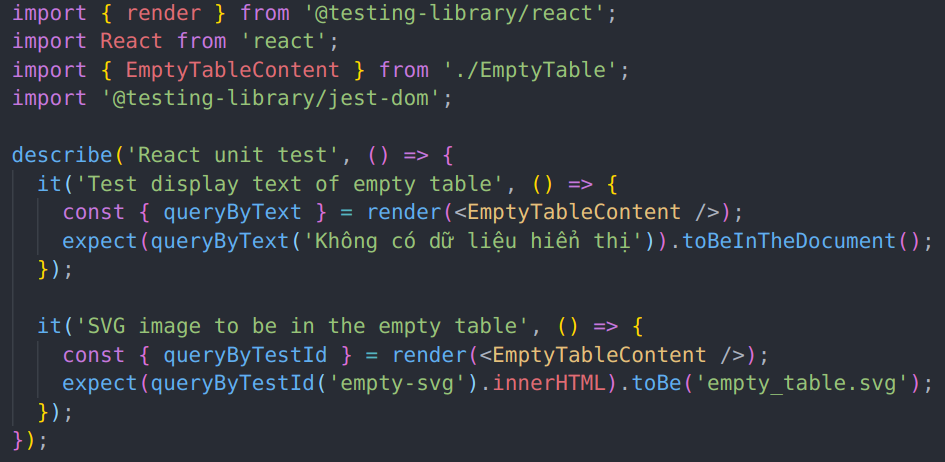
\includegraphics[width=0.8\textwidth]{/FE_unit_test/code.png}
			 		\centering
			 		\caption{Đoạn mã hiện thực}
			 	\end{figure}
			 	
			 	\begin{figure}[H]
			 		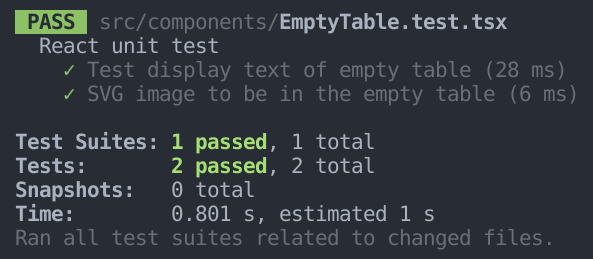
\includegraphics[width=0.8\textwidth]{/FE_unit_test/result.png}
			 		\centering
			 		\caption{Kết quả chạy 2 test case}
			 	\end{figure}
			 	
			 	\subsection{Tổng kết}
			 	Trên đây là những công nghệ nhóm đã dùng để hiện thực tương đối hoàn chỉnh phần front-end của hệ thống. Một hệ thống Front-end hoàn chỉnh không những chỉ cần những thành phần để hệ thống có thể chạy được mà cần phải có hệ thống track lỗi, thống kê truy cập vào website và đảm bảo lỗi thông qua unit test.
		
	
	\section{Back-end}
        \subsection{Giới thiệu kiến trúc Microservices}
        Trước khi Microservices xuất hiện, các ứng dụng thường phát triển theo mô hình Monolithic architecture (Kiến trúc một khối). Có nghĩa là tất cả các module (view, business, database) đều được gộp trong một project, một ứng dụng được phát triển theo mô hình kiến trúc một khối thường được phân chia làm nhiều module. Nhưng khi được đóng gói và cài đặt sẽ thành một khối (monolithic). Lợi ích của mô hình kiến trúc một khối đó là dễ dàng phát triển và triển khai. Nhưng bên cạnh đó nó cũng có nhiều hạn chế ví dụ như khó khăn trong việc bảo trì, tính linh hoạt và khả năng mở rộng kém, đặc biệt với những ứng dụng doanh nghiệp có quy mô lớn. Đó chính là lí do ra đời của kiến trúc Microservices. Với lý do đó nhóm sẽ chọn phát triển hệ thống theo kiến trúc Microservices.
        \begin{itemize}
            \item Những đặc điểm của Microservices
            \begin{itemize}
                \item \textbf{Decoupling} - Các service trong một hệ thống phần lớn được tách rời. Vì vậy, toàn bộ ứng dụng có thể dễ dàng được xây dựng, thay đổi và thu nhỏ.
                \item \textbf{Componentization} - Microservices được coi là các thành phần độc lập có thể dễ dàng thay thế và nâng cấp.
                \item \textbf{Business Capabilities} - Mỗi một thành phần trong kiến trúc microservice rất đơn giản và tập trung vào một nhiệm vụ duy nhất.
                \item \textbf{Autonomy} - Các lập trình viên hay các nhóm có thể làm việc độc lập với nhau trong quá trình phát triển.
                \item \textbf{Continous Delivery} - Cho phép phát hành phần mềm thường xuyên, liên tục.
                \item \textbf{Decentralized Governance} - Không có mẫu chuẩn hóa hoặc bất kỳ mẫu công nghệ nào. Được tự do lựa chọn các công cụ hữu ích tốt nhất để có thể giải quyết vấn đề.
                \item \textbf{Agility} - Microservice hỗ trợ phát triển theo mô hình Agile.
            \end{itemize}
            \item Ưu điểm\\\\
            Kiến trúc Microservices được sinh ra để khắc phục những hạn chế của kiến trúc một khối. Kiến trúc Microservices giúp đơn giản hóa hệ thống, chia nhỏ hệ thống ra làm nhiều service nhỏ lẽ dể dàng quản lý và triển khai từng phần so với kiến trúc nguyên khối. Phân tách rõ ràng giữa các service nhỏ. Cho phép việc mỗi service được phát triển độc lập. Cũng như cho phép lập trình viên có thể tự do chọn lựa technology stack cho mỗi service mình phát triển. mỗi service có thể được triển khai một cách độc lập (VD: Mỗi service có thể được đóng gói vào một docker container độc lập, giúp giảm tối đa thời gian deploy). Nó cũng cho phép mỗi service có thể được scale một cách độc lập với nhau. Việc scale có thể được thực hiện dễ dàng bằng cách tăng số instance cho mỗi service rồi phân tải bằng load balancer.
            \begin{itemize}
                \item \textbf{Independent Development} - Tất cả các service có thể được phát triển dễ dàng dựa trên chức năng cá nhân của từng service. Có thể chia nhỏ để phát triển độc lập.
                \item \textbf{Independent Deployment} - Có thể được triển khai riêng lẻ trong bất kỳ ứng dụng nào.
                \item \textbf{Fault Isolation} - Khi một service của ứng dụng không hoạt động, hệ thống vẫn tiếp tục hoạt động.
                \item \textbf{Mixed Technology Stack} - Các ngôn ngữ và công nghệ khác nhau có thể được sử dụng để xây dựng các service khác nhau của cùng một ứng dụng.
            \end{itemize}
            \item Nhược điểm
            \begin{itemize}
                \item Kiến trúc Microservices đang là một xu hướng, nhưng nó cũng có nhược điểm của nó. Microservice khuyến khích làm nhỏ gọn các service, nhưng khi chia nhỏ sẽ dẫn đến những thứ vụn vặt, khó kiểm soát. Hơn nữa chính từ đặc tính phân tán khiến cho các lập trình viên phải lựa chọn cách thức giao tiếp phù hợp khi xử lí request giữa các service.
                \item Hơn nữa việc quản lí nhiều database, và transaction giữa các service trong một hệ thống phân tán cũng là một khó khăn không nhỏ. Hay khi thực hiện test một service, bạn cũng cần test các service có liên quan.
                \item Triển khai microservice cũng sẽ phức tạp hơn so với ứng dụng kiến trúc một khối, cần sự phối hợp giữa nhiều service, điều này không đơn giản như việc triển khai WAR trong một ứng dụng kiến trúc một khối.
            \end{itemize}
            \item Với những ưu điểm và nhược điểm đã được nói ở trên nên nhóm đã quyết định sử dụng kiến trúc Microservices để xây dựng hệ thống của nhóm.
        \end{itemize}
		\subsection{Kiến trúc Microservicces}
		Các thành phần chính dự kiến xây dựng hệ thống trong Microservices
		\begin{itemize}
		    \item \textbf{Edge Server} - Để đưa các API services ra bên ngoài và để ngăn chặn truy cập trái phép vào các microservices nội bộ, chúng ta cần một edge server nơi tất cả request bên ngoài đi qua. Một edge server có thể tái sử dụng khả năng định tuyến động và cân bằng tải dựa trên service discovery được mô tả ở trên. Edge server sẽ hoạt động như một proxy ngược chủ động mà không cần cập nhật thủ công khi hệ thống nội bộ thay đổi.
		    \item \textbf{Dynamic Routing and Load Balancer} - Với chức năng service discovery, các thành phần định tuyến có thể sử dụng discovery API để tra cứu nơi mà microservice được yêu cầu được triển khai và các thành phần cân bằng tải có thể quyết định định tuyến yêu cầu tới instance nào nếu nhiều instance được triển khai cho một service được yêu cầu.
		    \item \textbf{Service Discovery} - Thay vì theo dõi thủ công những microservices nào được triển khai hiện tại và trên máy chủ và cổng nào, chúng ta cần chức năng Service Discovery cho phép microservices tự đăng ký khi khởi động thông qua API.
		    \item \textbf{Circuit Breaker} - Để tránh chuỗi sự cố, cần phải áp dụng Circuit Breaker pattern. Đây là một pattern dùng để ngắt một quá trình xử lý khi hệ thống gặp sự cố, để đảm bảo số lượng message bị lỗi không tăng cao, làm cho việc khắc phục trở nên khó khăn, cũng như có thể làm cho hệ thống bị xụp đổ hàng loạt do ảnh hưởng lẫn nhau.
		    \item \textbf{Monitoring} - Vì đã có circuit breakers, chúng ta có thể bắt đầu theo dõi trạng thái của chúng và thu thập số liệu thống kê thời gian chạy từ chúng để có được một bức tranh về tình trạng sức khỏe của hệ thống.
	        \item \textbf{Secure API} - Để bảo vệ các API services được expose ra bên ngoài sử dụng OAuth 2.0, quy trình của OAuth 2.0 có thể như sau:
	        \begin{itemize}
	            \item Một component mới có thể đóng vai trò như một Máy chủ ủy quyền (OAuth Authorization Server)
	            \item Các API services sẽ đóng vai trò như các Máy chủ tài nguyên (OAuth Resource Server)
	            \item Các Client bên ngoài gọi đến API services với tư cách là OAuth Clients
	            \item Edge server sẽ làm việc như một OAuth Token Relay: nó sẽ hoạt động như một OAuth Resource Serve, Nó sẽ chuyển các OAuth Access Tokens có trong request bên ngoài đến các API servicesr
	        \end{itemize}
	        \item \textbf{Central Configuration Server.} - Thay vì cấu hình cục bộ cho mỗi đơn vị triển khai (tức là microservice), chúng ta cần quản lý cấu hình tập trung. Chúng ta cũng cần một configuration API để các microservices có thể sử dụng để lấy thông tin cấu hình.
	        \item \textbf{Centralized Log Analysis} - Để có thể theo dõi messages và phát hiện khi chúng bị kẹt (stuck), chúng ta cần một chức năng phân tích log tập trung có khả năng tiếp cận với máy chủ và thu thập các tệp log mà mỗi services microservice tạo ra. Chức năng phân tích log lưu trữ thông tin log này trong cơ sở dữ liệu trung tâm và cung cấp khả năng tìm kiếm và dashboard. Lưu ý : Để có thể tìm thấy các messages liên quan, điều quan trọng là tất cả các microservices phải sử dụng id đồng nhất trong các log message.
		\end{itemize}
		Mô hình minh họa\\
		
		\newpage
		
		\begin{figure}[!ht]
			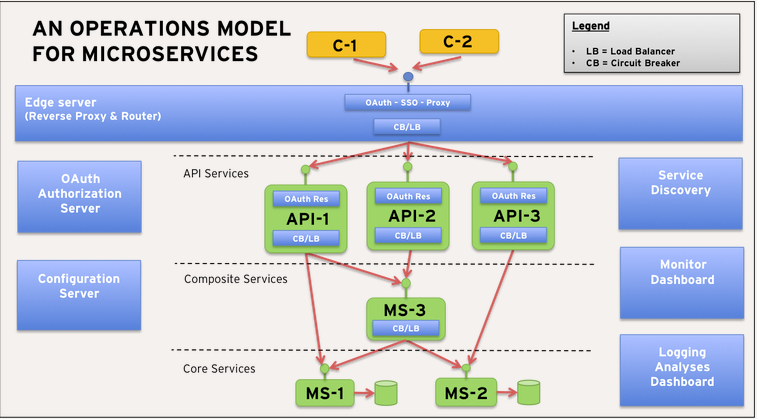
\includegraphics[width=0.8\textwidth]{Images/model-microservice.png}
			\centering
			\linebreak
			\caption{Mô hình Microservices}
		\end{figure}
		Các services dự kiến hệ thống của nhóm\\\\
		\begin{figure}[!ht]
			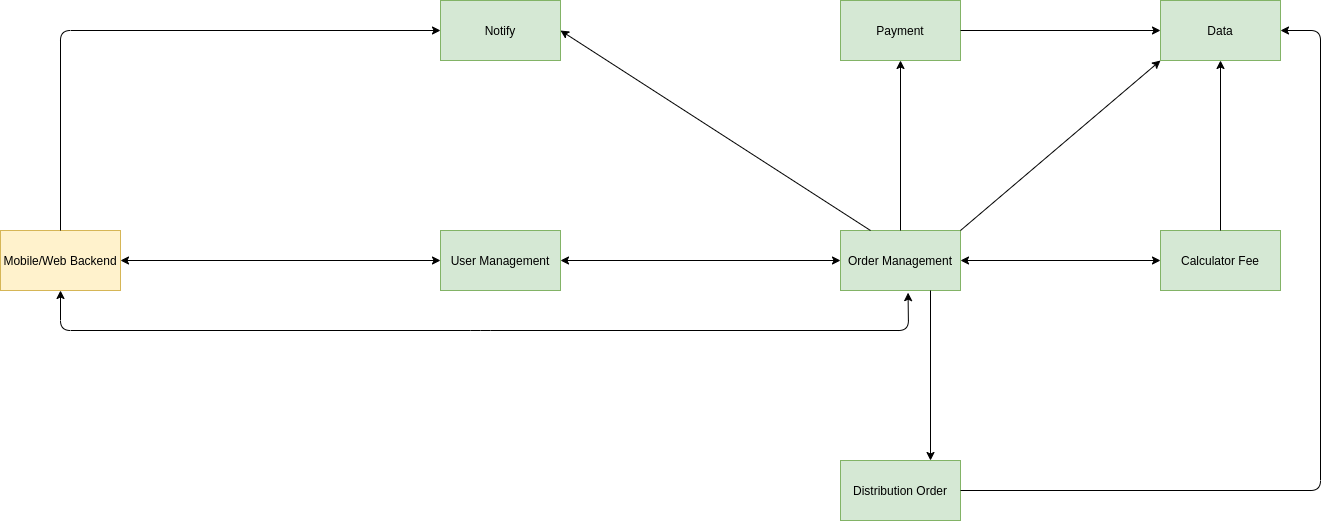
\includegraphics[width=0.8\textwidth]{Images/architecture.png}
			\centering
			\linebreak
			\caption{Mô hình services}
		\end{figure}\\
		\begin{itemize}
			\item \textbf{User Management}
			\begin{itemize}
				\item Service chịu trách nhiệm quản lý user trong hệ thống. Ở đây sẽ lưu trữ Database của user
				\item Mỗi khi user login vào hệ thống thì sẽ vào Service này để authen: Ban đầu user được yêu cầu sẽ nhập username và password, Sau khi authen là đúng user đó thì hệ thống sẽ sinh ra JWT (Json Web Token) để gửi trả về cho user. Sau này cứ mỗi request lên hệ thống thì user sẽ gửi kèm theo JWT để hệ thống có thể authen và author.
				\item User có thể get thông tin để có thể xem và chỉnh sửa
			\end{itemize}
			\item \textbf{Order Management}
			\begin{itemize}
				\item Service chịu trách nhiệm tạo Order cho user. Ở đây sẽ lưu trữ database về order.
				\item Mỗi khi có request lên thì service đi authen sau đó gọi qua service Calculator Fee để tính toán các chi phí rồi lưu Order đó vào DB với trạng thái là “Đơn nháp”. Sau đó sẽ gửi thông tin về Order cho user xác nhận. Sau khi nhận được request xác nhận của user thì trạng thái của đơn hàng chuyển thành “Chờ bàn giao”.
			\end{itemize}
			\item \textbf{Distribution Order}
			\begin{itemize}
				\item Service chịu trách nhiệm chia nhỏ các đơn hàng theo từng mặt hàng và chạy giải thuật để phân phối các đơn hàng cho tài xế.
				\item Ở đây lưu trữ Database về thông tin của đơn hàng sau khi được chia nhỏ thành các mặt hàng.
			\end{itemize}
			\item \textbf{Notify}
			\begin{itemize}
				\item Service chịu trách nhiệm quản lý các thông báo.
				\item Mobile/Web Backend sẽ liên tục gọi API getNotify để thông báo cho các user mỗi khi cần xác nhận bàn giao hàng
				\item Ngoài ra mỗi khi trạng thái đơn hàng thay đổi thì hê thống sẽ tự động gửi mail thông báo cho các user
			\end{itemize}
			\item \textbf{Calculator Fee}
			\begin{itemize}
				\item Service chịu trách nhiệm tính toán các khoản phí phát sinh
				\item Database lưu thông tin về phí của mỗi đơn hàng để các user có thể đối soát
			\end{itemize}
			\item \textbf{Payment}
			\begin{itemize}
				\item Service này sẽ liên kết với 1 bên thứ 3 như: ngân hàng, ví điện từ, .... để thực hiện chức năng thanh toán cho các user
			\end{itemize}
			\item \textbf{Data}
			\begin{itemize}
				\item Các service khác sẽ gửi data qua service này phục vụ cho việc tạo dashboard thống kê các hoạt động theo tuần, tháng, năm. Ngoài ra còn cung cấp data để team dev có thể monitor các service khác hoạt động như thế nào.
			\end{itemize}
		\end{itemize}
		\newpage
		\subsection{Công nghệ tổng quan}
		Bảng bên dưới là công nghệ dự tính thực hiện của nhóm:
		\begin{figure}[!ht]
			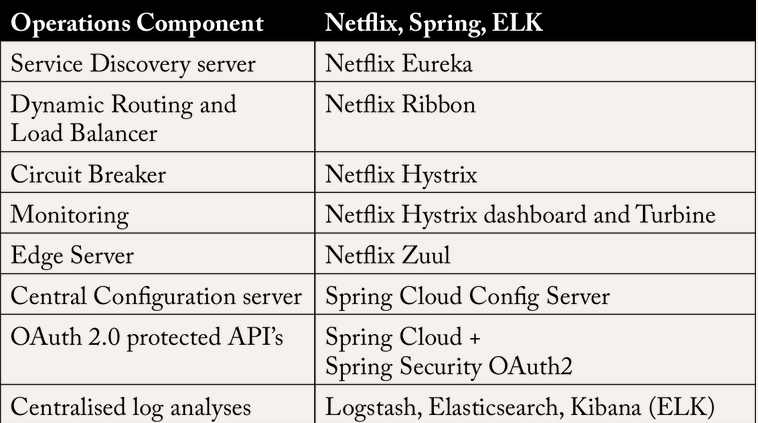
\includegraphics[width=0.8\textwidth]{Images/tech.png}
			\centering
			\linebreak
			\caption{Công nghệ sử dụng}
		\end{figure}\\
		Công nghệ nền tảng dự kiến sử dụng của nhóm: SPRING BOOT, SPRING CLOUD VÀ NETFLIX OSS
		\begin{itemize}
		    \item \textbf{Spring Boot} là một dự án nổi bật trong hệ sinh thái Spring Framework. Nếu như trước đây, công đoạn khởi tạo một dự án Spring khá vất vả từ việc khai báo các dependency trong file pom.xml cho đến cấu hình bằng XML hoặc annotation phức tạp, thì giờ đây với Spring Boot, chúng ta có thể tạo các ứng dụng Spring một cách nhanh chóng và cấu hình cũng đơn giản hơn.
		    \item \textbf{Spring Cloud} là nền tảng khá mới mẻ trong gia đình Spring.io dùng để xây dựng microservice một cách nhanh chóng. Spring Cloud cung cấp các công cụ cho các developer để nhanh chóng xây dựng một số common patterns trong các hệ thống phân tán (e.g. configuration management, service discovery, circuit breakers, intelligent routing, micro-proxy, control bus, one-time tokens, global locks, leadership election, distributed sessions, cluster state). Chúng sẽ hoạt động tốt trong bất kỳ môi trường phân tán nào, bao gồm máy tính xách tay của chính developer, các data center hoặc trên cloud.
		    \item Bản thân hệ sinh thái Spring không tự build hết tất cả các viên gạch cần để xây dựng ứng dụng Microservices. Thay vào đó, có một kho gạch dành cho Microservices được Netflix ban đầu phát triển trong nội bộ của họ để xây dựng dịch vụ xem phim trực tuyến nổi tiếng của họ và sau đó public ra dưới dạng open source với cái tên \textbf{Netflix OSS} (Open Source Software). Và Spring đơn giản chỉ làm nhiệm vụ wrap chúng lại và dùng trong hệ sinh thái của Spring (tất nhiên Spring nó còn wrap nhiều thằng khác nữa). Bằng cách kết hợp Spring Boot, Spring Cloud và Netflix OSS sẽ đủ cung cấp các công cụ và nguyên liệu cần thiết nhất để giúp bạn có thể nhanh chóng và dễ dàng xây dựng các Microservices của mình.
		\end{itemize}
		Công nghệ sử dụng cho Edge Server, Dynamic Routing and Load Balancer và Service Discovery
		\begin{itemize}
		    \item \textbf{Netflix Eureka} – Là một Service Discovery Server cho phép các dịch vụ microservices tự đăng ký mình vào danh sách các services hoạt động lúc khởi chạy. Server này sẽ chịu trách nhiệm lưu trữ và cung cấp thông tin của các service trong một hệ thống Microservice. Khi một service đăng ký thông tin với server, nó sẽ cung cấp các thông tin như host, port, trạng thái của nó. Và nó cũng thường xuyên gửi heartbeat message để thông báo tình trạng của mình cho server. Do đó, server này có thể dễ dàng cung cấp thông tin về các service khi chúng được gọi tới từ các service khác.
		    \item \textbf{Netflix Ribbon} – Với chức năng Dynamic Routing và Load Balancing có thể được sử dụng bởi Service client để tra cứu dịch vụ lúc runtime. Ribbon sử dụng thông tin có sẵn trong Eureka để định vị các instance thích hợp. Nếu tìm thấy nhiều hơn một instance, Ribbon sẽ áp dụng cân bằng tải để phân phối các reuqest đến các instance rảnh việc nhất. Ribbon không chạy dưới dạng một dịch vụ riêng biệt mà thay vào đó nó là một thành phần được nhúng trong mỗi Service client.
		    \item \textbf{Netflix Zuul} – Đóng vai trò như một Edge Server hoặc gatekeeper với thế giới bên ngoài, không cho phép bất kỳ yêu cầu bên ngoài trái phép nào đi qua. Các request đi tới services đều phải qua anh chàng Zuul này để check hàng trước. Zuul sử dụng Ribbon để tra cứu các dịch vụ sẵn có và định tuyến yêu cầu bên ngoài đến instance dịch vụ thích hợp. Trong bài đăng trên blog này, tôi sẽ chỉ sử dụng Zuul như một điểm vào (entry point).
		\end{itemize}
		Công nghệ sử dụng cho Circuit Breaker
		\begin{itemize}
		    \item \textbf{Netflix Hystrix} – Cung cấp khả năng ngắt mạch cho service consumer. Nếu một dịch vụ không đáp ứng (do timeout hoặc lỗi giao tiếp), Hystrix có thể chuyển hướng cuộc gọi đến phương thức dự phòng trong service consumer. Nếu một dịch vụ liên tục không hoạt động, Hystrix sẽ mở mạch và thực hiện fail fast (tức là gọi phương thức dự phòng mà không gọi đến service đó luôn) trên tất cả request tiếp theo cho đến khi dịch vụ “sống” trở lại. Để xác định khi nào một dịch vụ sống lại, lâu lâu nó sẽ thử bằng cách cho phép các request tới dịch vụ đó để xem nó sống lại hay chưa. Hystrix được cài đặt ở phía service consumber.
		\end{itemize}
		Công nghệ sử dụng cho Monitoring
		\begin{itemize}
		    \item \textbf{Netflix Hystrix dashboard và Netflix Turbine} –  Hystrix giúp kiểm soát sự tương tác giữa các dịch vụ bằng cách cung cấp khả năng chịu lỗi và khả năng chịu độ trễ. Nó cải thiện khả năng phục hồi tổng thể của hệ thống bằng cách cô lập các dịch vụ bị lỗi và ngăn chặn hiệu ứng phân tầng của các lỗi. Và Hystrix dashboard cung cấp trực quan tổng quát bộ ngắt mạch. Turbine là một công cụ mã nguồn mở của Netflix để tổng hợp nhiều luồng từ Hystrix vào một luồng duy nhất.
		\end{itemize}
		Công nghệ sử dụng cho Secure API
		\begin{itemize}
		    \item \textbf{Json Web Token(JWT)} - Là 1 tiêu chuẩn mở (RFC 7519) định nghĩa cách thức truyền tin an toàn giữa các thành viên bằng 1 đối tượng JSON. Thông tin này có thể được xác thực và đánh dấu tin cậy nhờ nó có chứa chữ ký số (digital signature). Phần chữ ký của JWT sẽ được mã hóa lại bằng HMAC hoặc RSA. Sử dụng JWT là cách tốt để áp dụng cơ chế bảo mật đối với các dịch vụ API RESTful mà có thể được sử dụng để truy cập vào cơ sở dữ liệu.
		\end{itemize}
		Công nghệ sử dụng cho Central Configuration Server
		\begin{itemize}
		    \item \textbf{Spring Cloud Config} là một mô-đun của Spring Cloud cung cấp việc lưu trữ và phục vụ các cấu hình phân tán trên nhiều ứng dụng và trên các môi trường phát triển (dev, staging, product, ...).. Spring Cloud Config hoạt động theo mô hình kiến trúc client - server, bao gồm: Spring Cloud Config Server và Spring Cloud Config Client.
		    \begin{itemize}
		        \item \textbf{Spring Cloud Config Server}: Các property của các ứng dụng Spring (được lưu trong các property source như file properties hoặc file YAML) được tập trung trên một hệ thống backend: Git repository (mặc định), File System, Vault, JDBC, Redis... Nhiệm vụ của Spring Config Server là pull các property này về và dùng EnvironmentRepository để lưu trữ. EnvironmentRepository cung cấp các đối tượng Spring Environment.Sau đó cung cấp các property cho Config Client thông qua các HTTP resource-based API (HTTP Method là GET).
		        \item \textbf{Spring Cloud Config Client}: Đây chính là các ứng dụng Spring đã tách biệt các property. Khi startup, Config Client sẽ đọc các property từ API của Config Server và khởi tạo đối tượng Environment với property source phù hợp.
		    \end{itemize}
		\end{itemize}
		Công nghệ sử dụng cho Centralized Log Analysis
		\begin{itemize}
		    \item \textbf{Logstash} - Có thể thu thập các sự kiện nhật ký từ nhiều loại nguồn bằng cách sử dụng các plug-ins đầu vào, chuyển đổi nó sang định dạng bạn thích bằng cách sử dụng các plug-ins filter và codec và gửi nó đến một số điểm đến bằng các plug-ins đầu ra.
		    \begin{itemize}
		        \item \textbf{Input}: tiếp nhận/thu thập dữ liệu sự kiện log ở dạng thô từ các nguồn khác nhau như file, redis, rabbitmq, beats, syslog,….
		        \item \textbf{Filter}: Sau khi tiếp nhận dữ liệu sẽ tiến hành thao tác dữ liệu sự kiện log (như thêm, xoá, thay thế,.. nội dung log) theo cấu hình của quản trị viên để xây dựng lại cấu trúc dữ liệu log event theo mong muốn.
		        \item \textbf{Output}: Sau cùng sẽ thực hiện chuyển tiếp dữ liệu sự kiện log về các dịch vụ khác như Elasticsearch tiếp nhận lưu trữ log hoặc hiển thị log,..
		    \end{itemize}
		    \item \textbf{Elasticsearch} - Là một cơ sở dữ liệu tìm kiếm toàn văn bản được phân phối và có thể mở rộng, cho phép bạn lưu trữ và tìm kiếm khối lượng lớn các sự kiện nhật ký. Thay vì tìm kiếm trên file, trên các database như MySQL, Oracle, MongoDB… thì chuyển dữ liệu đó sang Elasticsearch và thực hiện tìm kiếm trên Elasticsearch sẽ mang lại hiệu quả rất lớn, đặc biệt là trong những trường hợp dữ liệu log lớn.
		    \begin{itemize}
		        \item Ưu điểm
		        \begin{itemize}
		            \item Tìm kiếm dữ liệu rất nhanh chóng, mạnh mẽ dựa trên Apache Lucene ( near-realtime searching)
		            \item Có khả năng phân tích dữ liệu
		            \item Khả năng mở rộng theo chiều ngang
		            \item Hỗ trợ tìm kiếm mờ tức là từ khóa tìm kiếm có thể bị sai lỗi chính tả hay không đúng cú pháp thì vẫn có khả năng elasticsearch trả về kết quả tốt.
		            \item Hỗ trợ Structured Query DSL (Domain-Specific Language ), cung cấp việc đặc tả những câu truy vấn phức tạp một cách cụ thể và rõ ràng bằng JSON.
		            \item Hỗ trợ nhiều Elasticsearc client như Java, PhP, Javascript, Ruby, .NET, Python
		        \end{itemize}
		        \item Nhược điểm
		        \begin{itemize}
		            \item Trong elasticsearch không có khái niệm database transaction , tức là nó sẽ không đảm bảo được toàn vẹn dữ liệu trong các hoạt động Insert, Update, Delete.Tức khi chúng ta thực hiện thay đổi nhiều bản ghi nếu xảy ra lỗi thì sẽ làm cho logic của mình bị sai hay dẫn tới mất mát dữ liệu. Đây cũng là 1 phần khiến elasticsearch không nên là database chính.
		            \item Không thích hợp với những hệ thống thường xuyên cập nhật dữ liệu. Sẽ rất tốn kém cho việc đánh index dữ liệu.
		            \item Elasticsearch được thiết kế cho mục đích search, do vậy với những nhiệm vụ khác ngoài search như CRUD thì elastic kém thế hơn so với những database khác như Mongodb, Mysql ….
		        \end{itemize}
		    \end{itemize}
		    \item \textbf{Kibana} - Cho phép bạn hình dung và phân tích các sự kiện nhật ký của bạn được lưu trữ trong Elasticsearch.
		    \begin{itemize}
		        \item Cung cấp biểu đồ tương tác: Kibana cung cấp các biểu đồ và báo cáo trực quan mà bạn có thể sử dụng để điều hướng tương tác thông qua một lượng lớn dữ liệu. Bạn có thể tự động kéo các cửa sổ thời gian, phóng to, thu nhỏ các tập hợp dữ liệu cụ thể và xem chi tiết các báo cáo để trích xuất thông tin chi tiết có thể hành động từ dữ liệu của bạn.
		        \item Tập hợp và bộ lọc dựng sẵn: Sử dụng các tập hợp và bộ lọc dựng sẵn của Kibana, bạn có thể chạy nhiều loại phân tích như biểu đồ, truy vấn N hàng đầu và xu hướng.
		        \item Bảng điều khiển dễ dàng truy cập: có thể dễ dàng thiết lập bảng điều khiển và báo cáo và chia sẻ chúng với những người khác. Chỉ cần một trình duyệt để xem và khám phá dữ liệu.
		        \item Công cụ trình bày Canvas: Canvas kết hợp dữ liệu với màu sắc, hình dạng, và trí tưởng tượng để mang lại sự hiển thị dữ liệu động, đa trang, pixel hoàn hảo cho màn hình lớn và nhỏ, làm cho dữ liệu tuyệt vời hơn.
		        \begin{figure}[!ht]   			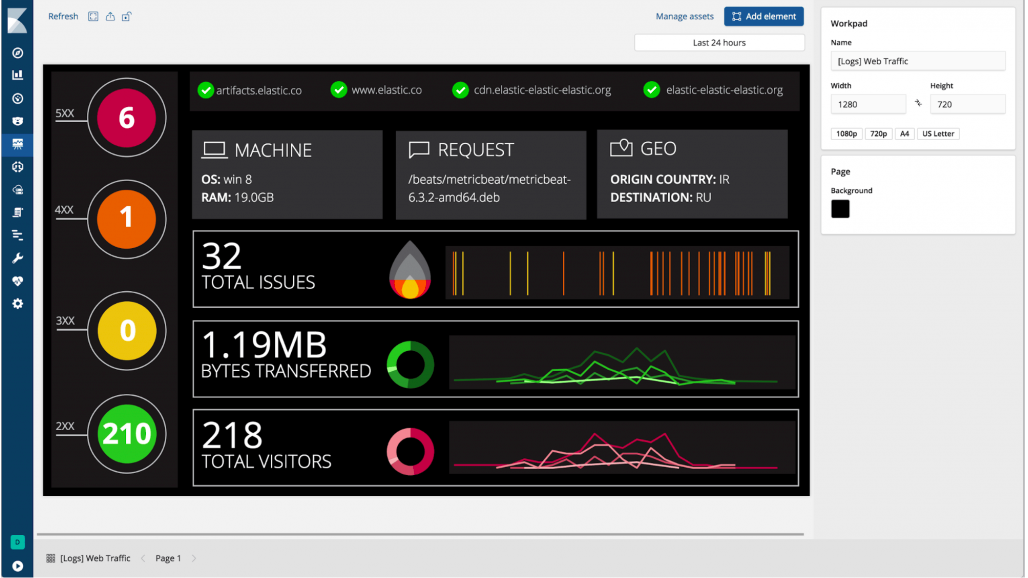
\includegraphics[width=0.8\textwidth]{Images/canvas.png}
    			\centering
    			\linebreak
    			\caption{Canvas}
		        \end{figure}\\
		        \newpage
		        \item Dev Tools: Chứa các công cụ phát triển giúp bạn tương tác với dữ liệu dễ dàng hơn\\
		        \begin{figure}[!ht]   			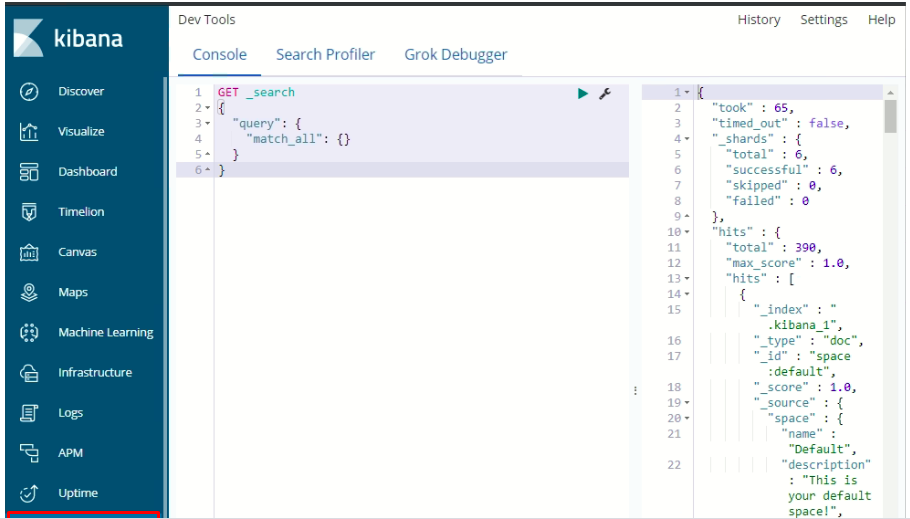
\includegraphics[width=0.8\textwidth]{Images/devtool.png}
    			\centering
    			\linebreak
    			\caption{Dev Tool}
		        \end{figure}\\
		    \end{itemize}
        \subsection{Kiến trúc RESTful API}
		    
		    RESTful API là một tiêu chuẩn dùng trong việc thiết kế các API cho ứng dụng web để quản lý resource. RESTful là một trong những kiểu thiết kế API được sử dụng phổ biến ngày nay để cho các ứng dụng (web, mobile, web service...) khác nhau có thể giao tiếp với nhau.
		    
		    Khi làm việc với server sẽ gồm 4 hoạt động thiết yếu đó là: lấy dữ liệu, tạo mới, cập nhật, xóa dữ liệu.
		    
		    REST hoạt động chủ yếu dựa vào giao thức HTTP. Mỗi trong 4 hoạt động cơ bản trên sẽ sử dụng những phương thức HTTP riêng (HTTP method):
		    \begin{itemize}
		        \item POST (CREATE) : Tạo mới một tài nguyên.
		        \item GET (READ) : Trả về một tài nguyên hoặc một danh sách tài nguyên.
		        \item PUT (UPDATE) : Cập nhật, thay thế thông tin cho tài nguyên.
		        \item DELETE (DELETE) : Xóa một tài nguyên.
		    \end{itemize}
		    REST là một kiến trúc thống nhất giúp thiết kế các website để có thể dễ dàng quản lý các tài nguyên. Nó không phải là một quy luật buộc bạn phải tuân theo mà đơn giản là một kiến trúc được đề xuất ra và kiến trúc này hiện đang được sử dụng rất phổ biến vì tính đơn giản, dễ hiểu và rất ưu việt của nó. Với các ứng dụng web được thiết kế sử dụng RESTful, ban có thể dễ dàng biết được URL và HTTP method để quản lý một resource
		    
		    Ưu điểm
		  
	        \begin{itemize}
	            \item REST cũng có ưu điểm khi sử dụng giao thức stateless (không trạng thái). Hệ thống này không sử dụng session, cookie, không cần biết những thông tin đó trong mỗi lần request đến máy chủ ngoài. Điều này giúp REST giảm tải cho máy chủ ngoài, nâng cao hiệu suất làm việc.
	            \item Tính khả biến: với các hệ thống cần thay đổi các tài nguyên liên tục, sử dụng REST với việc tạo request đơn giản sẽ giúp mọi chuyện trở nên đơn giản hơn.
	            \item Tính mở rộng: các hệ thống REST có khả năng mở rộng rất cao nhờ sự tách biệt giữa các thành phần và các quy ước giao tiếp được quy định sẵn.
	            \item Tính linh hoạt: việc chuẩn hoá interface giúp hệ thống trở nên linh hoạt hơn, có thể sử dụng cho cho nhiều nền tảng khác nhau, mobile, web,...
	            \item Trong sáng: trong giao tiếp giữa các thành phần, các request trở nên rất rõ ràng, dễ hiểu.
	        \end{itemize}
	        
		    Nhược điểm
		    
	        \begin{itemize}
	            \item REST Chỉ hoạt động trên các giao thức HTTP.
	        \end{itemize}
	        \subsection{Công nghệ gRPC}
		    
		    gRPC có thể được xem là một giao thức request và response thông thường tuy nhiên nó được dùng cho việc giao tiếp giữa các server với nhau (server-server) nhiều hơn là client-server. Việc này có ý nghĩa rất quan trọng vì trong các hệ thống phân tán, request sẽ được xử lý bởi nhiều server hơn là một server. Ví dụ thường thấy nhất chính là kiến trúc Microservices.
		    
		    Thông thường mỗi khi có request từ client, thì request đó có thể được xử lý bởi nhiều server khác nhau thì mới trả kết quả về cho client. Chính sự giao tiếp giữa các server có thể làm tăng thời gian xử lý của request đó. Chính điều này thúc đẩy sự ra đời của gRPC nhằm tăng hiệu suất giao tiếp giữa các server với nhau.
		    
		    gRPC sử dụng Protocol Buffer và giao thức HTTP/2 để transfer data thay vì JSON/XML và giao thức HTTP/1.1 truyền thống nên tốc độ được gia tăng đáng kể.
		    \newpage
    	    \begin{figure}[!ht]   			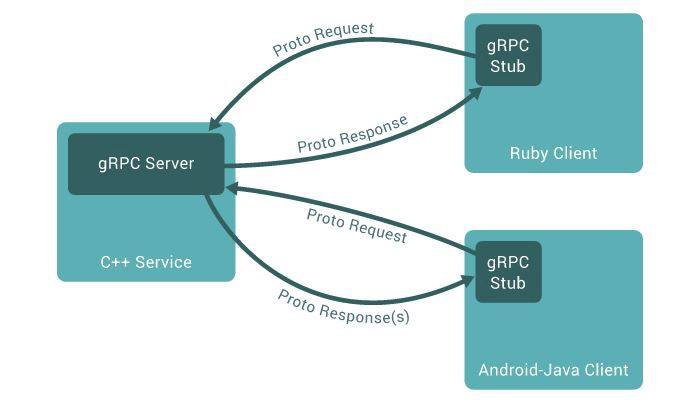
\includegraphics[width=0.8\textwidth]{Images/gRPC.jpg}
    		\centering
    		\linebreak
    		\caption{gRPC}
	        \end{figure}
		    
		    Cách hoạt động: Ở phía server sẽ hiện thực cách xử lý method mà nó cung cấp, sau đó ở phía client chỉ việc gửi các tham số cùng với tên method muốn gọi. Sau khi nhận được request phía server sẽ dựa trên các tham số và tên method để thực thi. Sau khi có kết quả thì server sẽ trả về cho client.
		    
		    Ưu điểm
		    
		    \begin{itemize}
		        \item Dựa trên file protobuf thì dữ liệu sẽ được serialize ra dạng binary nên tốc độ truyền đi trong mạng rất nhanh.
		        \item Sử dụng HTTP/2 giúp tận dụng tối đa băng thông, giúp client trải nghiệm sản phẩm tốt hơn.
		    \end{itemize}
		    
		    Nhược điểm
		    
		    \begin{itemize}
		        \item Chưa được hỗ trợ toàn diện
		        \item Khó hiện thực
		        \item Dữ liệu ở dạng binary nên khó debug
		        \item Các tool để test API như Postman, curl, … chưa hỗ trợ
		    \end{itemize}
		    
		    Trong quá trình nghiên cứu và tìm hiểu thì nhóm nhận thấy có rất nhiều công nghệ hỗ trợ cho việc giao tiếp giữa client-server, server-server như: SOAP, RESTful API, gRPC,...

            Đối với SOAP thì nhóm nhận thấy nó có một số nhược điểm như: Nó duy trì trạng thái (stateful) khiến chúng ta tiêu tốn tài nguyên cho các metadata, không phổ biến như REST cho các ứng dụng web và chỉ sử dụng XML vì thế nhóm quyết định chọn RESTful API để giao tiếp giữa client-server, server-server. Ngoài ra còn sử dụng gRPC cho server-server nhằm làm tăng tốc độ quá trình truyền tải dữ liệu.
            \subsection{MySQL}
            
            MySQL là hệ quản trị cơ sở dữ liệu tự do nguồn mở phổ biến nhất thế giới và được các nhà phát triển rất ưa chuộng trong quá trình phát triển ứng dụng. Vì MySQL là cơ sở dữ liệu tốc độ cao, ổn định và dễ sử dụng, có tính khả chuyển, hoạt động trên nhiều hệ điều hành cung cấp một hệ thống lớn các hàm tiện ích rất mạnh. Với tốc độ và tính bảo mật cao, MySQL rất thích hợp cho các ứng dụng có truy cập CSDL trên internet.
            
            Ưu điểm
            
            \begin{itemize}
                \item Dễ sử dụng: MySQL là cơ sở dữ liệu tốc độ cao, ổn định, dễ sử dụng và hoạt động trên nhiều hệ điều hành.
                \item Độ bảo mật cao:  MySQL rất thích hợp cho các ứng dụng có truy cập CSDL trên Internet khi sở hữu nhiều nhiều tính năng bảo mật thậm chí là ở cấp cao.
                \item Đa tính năng: MySQL hỗ trợ rất nhiều chức năng SQL được mong chờ từ một hệ quản trị cơ sở dữ liệu quan hệ cả trực tiếp lẫn gián tiếp.
                \item Khả năng mở rộng và mạnh mẽ: MySQL có thể xử lý rất nhiều dữ liệu và hơn thế nữa nó có thể được mở rộng nếu cần thiết.
            \end{itemize}
            
            Nhược điểm
            
            \begin{itemize}
                \item Khả năng scale rất khó và tốn chi phí: Nếu số bản ghi của bạn lớn dần lên thì việc truy xuất dữ liệu của bạn là khá khó khăn, khi đó chúng ta sẽ phải áp dụng nhiều biện pháp để tăng tốc độ truy xuất dữ liệu như là chia tải database này ra nhiều server.	
            \end{itemize}	
            \subsection{Cassandra}
            
            Ngày nay, các dịch vụ trên Internet phải xử lí khối lượng dữ liệu rất lớn. Hầu hết dữ liệu sẽ được lưu trữ phân tán trên nhiều máy chủ khác nhau. Vì vậy, các hệ quản trị cơ sở dữ liệu quan hệ (RDBMS) tỏ ra không còn phù hợp với các dịch vụ như thế này nữa. Người ta bắt đầu nghĩ tới việc phát triển các DBMS mới phù hợp để quản lý các khối lượng dữ liệu phân tán này. Các DBMS này thường được gọi là NoSQL. Một đại diện nổi bật của các NoSQL là Cassandra.
            
            Cassandra ban đầu được tạo ra bởi Facebook. Sau đó nó đã được tặng cho Quỹ Apache và tháng 2 năm 2010 và được nâng cấp lên thành dự án hàng đầu của Apache. Cassandra là một cơ sở dữ liệu phân tán kết hợp mô hình dữ liệu của Google Bigtable với thiết kế hệ thống phân tán như bản sao của Amazon Dynamo. 
            
            Ưu điểm
            
            \begin{itemize}
                \item Khả năng chịu lỗi cao: Do dữ liệu khi lưu vào cassandra sẽ được nhân bản và lưu trữ trên các node khác nhau. Vì thế nếu có 1 node nào đó chứa dữ liệu cần đọc down thì hệ thống có thể điều phối để đọc dữ liệu đó ở node khác.
                \item Kiến trúc không có SPOF (Single Point Of Failure): Bởi vì trong Cassandra không có node chính. Các node kết hợp với nhau tạo thành 1 Ring. Và các node đều có vai trò như nhau. Cho nên hệ thống sẽ không dừng lại khi một hoặc một số node cho phép trong mạng down.
                \item Hỗ trợ nhiều ngôn ngữ khác nhau: Do cassandra thu thập dữ liệu bằng một framework có tên là Thrift và Thrift có một cơ chế để giao tiếp với các ngôn ngữ khác nhau.
                \item Dễ dàng scale và mở rộng: Cassandra có hệ thống cluster bao gồm nhiều node được kết nối với nhau tạo thành Ring. Vì thế để mở rộng khả năng lưu trữ và xử lý thì ra chỉ việc thêm node vào mà không ảnh hưởng đến các node khác trong mạng do Cassandra sử dụng một thuật toán có tên là Consistency Hashing để phân chia dữ liệu đến các node trong Ring.
                \item Tốc độ đọc/ghi nhanh: Do Cassandra không có ràng buộc giữa các table như RDBMS nên việc truy xuất cực kì nhanh.
            \end{itemize}
            
            Nhược điểm
            
            \begin{itemize}
                \item Cassandra không hỗ trợ cho việc tính toán trên storage. Ở đây ta có thể tính toán ở application trước khi lưu vào Database.
                \item Do dữ liệu được phân tán trên các node nên dữ liệu giữa các có thể không giống nhau (chỉ đảm bảo Eventually Consistency). Ở đây ta có thể set Consistency Level để quản lý việc đọc/ghi dữ liệu. Nếu ta ưu tiên về độ chính xác thì có thể set là QUORUM hay ALL nhưng bù lại sẽ tăng thời gian phản hồi. Ngược lại, nếu ưu tiên về tốc độ thì ta có thể set là ONE, TWO, … nhưng ở đây ta phải đánh đổi về độ chính xác của dữ liệu.
            \end{itemize}
            
            Kết luận
            
            \begin{itemize}
                \item Sau quá trình tìm hiểu và thử nghiệm thì nhóm nhận thấy một số điều. Đối với MySQL thì có một số ưu điểm như: dễ sử dụng, hỗ trợ transaction, hỗ trợ ràng buộc nghiêm ngặt, … nhưng nhóm cũng nhận thấy một nhược điểm rất lớn đó là khó scale. Đối với lương dữ liệu còn ít thì việc thực thi các câu truy vấn trong MySQL diễn ra rất trơn tru nhưng khi dữ liệu càng phình to ra thì việc query trở nên nặng nề và rất chậm. Vì thế nhóm sẽ sử dụng MySQL để lưu các config ít thay đổi trong hệ thống. Ví dụ như: path, port của service khác, mã lỗi, …
                \item Ngoài ra với những ưu điểm của Cassandra thì nhóm sẽ sử dụng để lưu trữ các dữ liệu về business, các dữ liệu về log, dữ liệu về người dùng, … để có thể đảm bảo tính chịu lỗi và sẵn sàng.
            \end{itemize}
            \subsection{Redis}
            
            Ngày nay việc tăng tốc truy vấn để đáp ứng request một cách nhanh chóng đang dần trở nên phổ biến. Mỗi khi muốn truy xuất lấy dữ liệu từ Database thì ta phải xuống ổ cứng, mà tốc độ đọc/ghi dữ liệu từ ổ cứng chậm hơn rất nhiều so với RAM (khoảng 200 lần). Vì thế người ta nghĩ ra cách lưu dữ liệu thường xuyên truy xuất lên RAM để có thể phản hồi request của client với tốc độ nhanh nhất. Từ đó, Redis ra đời và được biết đến như là 1 cache database rất phổ biến trên thế giới.
            
            Đặc điểm
            
            \begin{itemize}
                \item Là cơ sở dữ liệu NoSQL, lưu trữ dữ liệu dưới dạng KEY-VALUE
                \item Lưu trữ dữ liệu trên RAM, giúp việc truy xuất dữ liệu cực kì nhanh chóng.
                \item Hỗ trợ nhiều cấu trúc dữ liệu cơ bản như Hash, List, Set, Sorted Set, String,....
                \item Hỗ trợ cơ chế Pub/Sub messaging.
                \item Hỗ trợ cơ chế Persistence giúp bảo vệ khỏi mất mát dữ liệu khi có sự cố xảy ra
            \end{itemize}
            
            Nhờ đặc điểm giúp giảm thời gian truy vấn, nên Redis có tác dụng rất mạnh mẽ trong việc sử dụng làm cache có các ứng dụng web.
            
            Ưu điểm
            
            \begin{itemize}
                \item Dữ liệu lưu trữ trong bộ nhớ
                \item Hỗ trợ nhiều cấu trúc dữ liệu linh hoạt, phù hợp với nhiều ngôn ngữ lập trình như: String, List, Hash, Set, ZSet, …
                \item Đơn giản và dễ sử dụng
                \item Sao chép và độ bền: Redis hỗ trợ xây dựng theo nhiều kiến trúc khác nhau tùy vào nhu cầu và mục đích sử dụng. Ví dụ như: master-slave thì slave sẽ sao lưu dữ liệu từ master. Nếu master bị down thì slave sẽ được đưa lên thay thế master nhằm tránh việc bị mất mát dữ liệu, ngoài ra còn có thể phân chia việc đọc/ghi dữ liệu. Slave sẽ xử lý các request đọc dữ liệu, còn master sẽ xử lý các request ghi dữ liệu.
                \item Khả năng mở rộng: Redis là dự án open source được cộng đồng đông đảo ủng hộ. Không có giới hạn về nhà cung cấp hoặc công nghệ vì thế Redis còn có thể mở rộng và cải tiến thêm nhiều tính năng hơn nữa.
            \end{itemize}
            
            Nhược điểm
            
            \begin{itemize}
                \item Do Redis lưu trữ dữ liệu trong RAM nên phần nào vẫn có nguy cơ mất mát dữ liệu.
                \item Mỗi lần chỉnh sửa hay thêm dữ liệu thì ta đồng thời phải thêm/sửa vào cả database và Redis nên có thể mang đến một số phức tạp.
                \item Key trong Redis có giới hạn: Vì thế trong quá trình lưu trữ nếu không cẩn thận có thể gây chết server Redis
                \item Cache Invalidation: Khó khăn khi loại bỏ đi dữ liệu không còn được sử dụng trong Redis. Thông thường người ta thường đặt Time to live cho mỗi dữ liệu cache tùy theo tần số thay đổi, tần suất truy vấn và mức độ quan trọng của dữ liệu.
            \end{itemize}
            
            Ở đây nhóm sẽ sử dụng Redis cho mục đích cache là chủ yếu. Bởi vì có một số thông tin thường xuyên được request nhiều lần. Nếu để trong database được lưu ở ổ cứng thì dẫn tới việc làm tăng thời gian truy xuất, có thể dẫn tới chết database. Ngoài ra do Redis hỗ trợ thêm cơ chế Persistence để định kỳ sao lưu dữ liệu lên ổ cứng nên có thể phần nào đảm bảo dữ liệu không bị mất mát khi có sự cố xảy ra.
            
            \subsection{ActiveMQ}
            
            Message queue là một kiến trúc cung cấp giao tiếp không đồng bộ. Ý nghĩa của queue ở đây chính là 1 hàng đợi chứa message chờ để được xử lý tuần tự theo cơ chế vào trước thì ra trước (FIFO - First In First Out). Một message là các dữ liệu cần vận chuyển giữa người gửi và người nhận. Ta có thể hiểu đơn giản việc sử dụng message queue cũng giống như việc ta đi gửi thư vậy. Lúc đến bưu điện ta chỉ việc bỏ thư vào hòm mà không cần quan tâm lúc nào thư sẽ được gửi đi mà chỉ biết là nó chắc chắn sẽ được xử lý. Đây là một ví dụ về việc giao tiếp bất đồng bộ.
            
            \newpage
            
             \begin{figure}[!ht]   			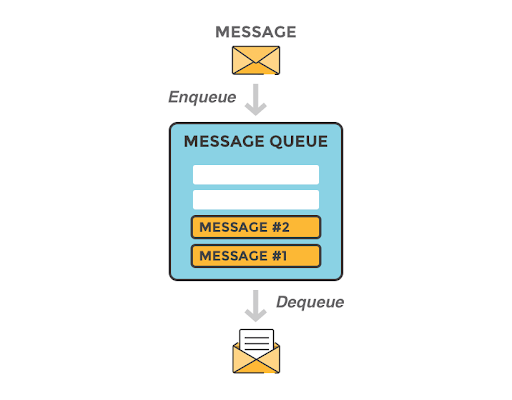
\includegraphics[width=0.8\textwidth]{Images/message.png}
			\centering
			\linebreak
			\caption{Active MQ}
	        \end{figure}
		        
            Kiến trúc cơ bản Message Queue
            
            \begin{itemize}
                \item Message: Là thông tin cần gửi đi
                \item Producer: Là thành phần sẽ gửi message
                \item Consumer: Là thành phần nhận message
                \item Message Queue: Nơi chứa message, cho phép producer và consumer có thể trao đổi với nhau.
            \end{itemize}
            
            Các loại Message Queue
            
            \begin{itemize}
                \item Point-to-point: Tức là message chỉ được consumer bởi 1 thành phần duy nhất
                
                \newpage
                
                \begin{figure}[!ht]   			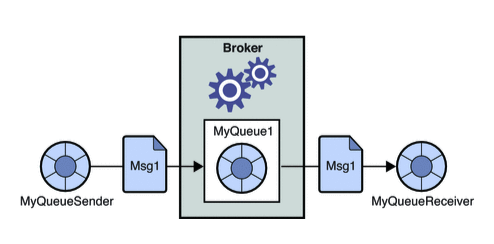
\includegraphics[width=0.8\textwidth]{Images/PTP.png}
        		\centering
        		\linebreak
        		\caption{Point-to-point}
                \end{figure}
                
                \item Publisher-Subcriber: Ở đây ta có thể có nhiều consumer cùng consume 1 message giống nhau khi chúng cùng subcriber vào 1 topic.
                
                \begin{figure}[!ht]   			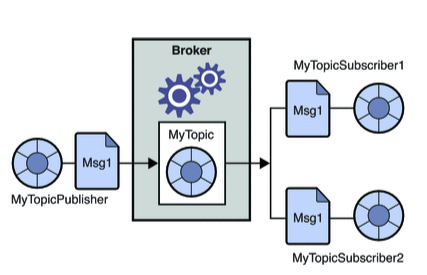
\includegraphics[width=0.8\textwidth]{Images/PS.png}
        		\centering
        		\linebreak
        		\caption{Publisher-Subcriber}
                \end{figure}
                
            \end{itemize}
            
            Ưu điểm
            
            \begin{itemize}
                \item Đảm bảo 1 message chỉ được xử lý đúng 1 lần duy nhất: Mỗi khi consumer lấy được message thì nó sẽ gửi 1 ACK về cho Broker, sau khi nhận được tín hiệu ACK thì Broker sẽ tiến hành xóa message đó đi để tránh việc 1 message được xử lý 2 lần.
                \item Nhắn tin không đồng bộ: Phù hợp với những việc không cần phải xử lý ngay lập tức. Lúc đó ta cứ đưa message vào queue rồi đi xử lý các công việc tiếp theo. Nhằm giảm response time đối với client.
                \item Tăng khả năng sẵn sàng: Giả sử ta có 2 service và lúc đó 1 trong 2 service đang trong trạng thái không hoạt động. Thì lúc đó hệ thống vẫn có thể hoạt động bình thường. Ta giữ các message trong queue đến khi service hoạt động lại thì nó consume message và tiếp tục công việc xử lý của nó
                \item Dễ dàng mở rộng: Mỗi khi lượng request tăng cao. Producer bắn message nhanh hơn tốc độ xử lý cả consumer thì lúc này ta chỉ đơn giản là thêm consumer vào để tăng tốc độ xử lý. Chú ý: Lúc này ta cần set tất cả các consumer chung 1 group-id để tránh việc 1 message có thể được xử lý nhiều lần.
            \end{itemize}
            
            Nhược điểm
            
            \begin{itemize}
                \item Làm phức tạp hệ thống: Khi thêm 1 thành phần thì ta phải chấp nhận việc xử lý phức tạp và có thể xảy ra sai sót trong quá trình xử lý.
                \item Producer và Consumer phải thống nhất về format của message: Mặc dù cả producer và consumer không quan tâm đến nhau (chỉ cần gửi message vào queue rồi thằng kia tới lấy) nhưng cả 2 cần có chung 1 format message để có thể dễ dàng xử lý sau khi consume.
                \item Monitor Queue: Ta cần phải theo dõi queue để biết được tính trạng hiện tại, queue có đầy hay không, có bị crash không để đưa ra phương án xử lý.
            \end{itemize}
            
            Cách sử dung
            
            Mặc dù message queue rất phù hợp để giao tiếp giữa các service trong hệ thống microservice. Nhưng ở đây nhóm chỉ sử dụng message để hiện thực cơ chế bất đồng bộ khi xử lý request tại một service cụ thế. Ví dụ như: Sau khi xử lý request của client ta cần vào Database để cập nhật lại status của đơn hàng nhưng việc truy xuất vào Database ngay thời điểm đó là không cần thiết. Ta có thể đưa message vào queue và sau đó trả kết quả về cho client ngay lập tức. Điều đó giúp ta tránh được việc truy xuất Database quá lâu sẽ ảnh hưởng đến trải nghiệm của người dùng.
            
            \subsection{Kafka}
            
            Kafka là dự án mã nguồn mở, đã được đóng gói hoàn chỉnh, khả năng chịu lỗi cao và là hệ thống nhắn tin nhanh. Vì tính đáng tin cậy của nó, kafka đang dần được thay thế cho hệ thống nhắn tin truyền thống. Nó được sử dụng cho các hệ thống nhắn tin thông thường trong các ngữ cảnh khác nhau. Đây là hệ quả khi khả năng mở rộng ngang và chuyển giao dữ liệu đáng tin cậy là những yêu cầu quan trọng nhất.
            
            Để có thể hiểu rõ vai trò của Kafka ta có thể xem ảnh sau
            
            \begin{figure}[!ht]   			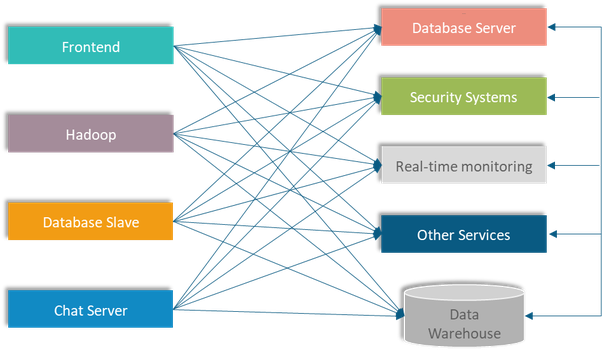
\includegraphics[width=0.8\textwidth]{Images/Kafka1.png}
    		\centering
    		\linebreak
    		\caption{Vai trò Kafka}
            \end{figure}
            
            Thông thường việc giao tiếp giữa các thành phần trong hệ thống diễn ra hết sức phức tạp. Điều này làm tăng chi phí giám sát và làm giảm hiệu suất của hệ thống.
            
            Và từ đó Kafka ra đời giúp chúng ta đơn giản đi việc giao tiếp giữa các thành phần trong hệ thống với nhau.
            
             \begin{figure}[!ht]   			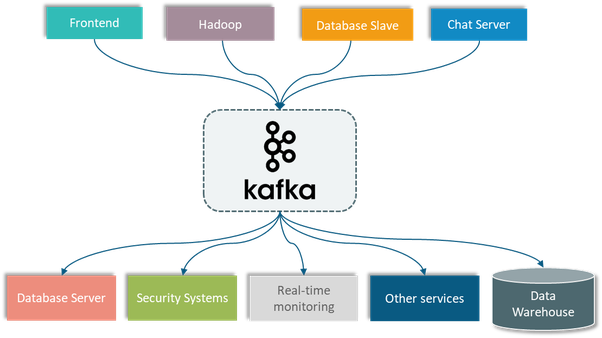
\includegraphics[width=0.8\textwidth]{Images/Kafka3.png}
    		\centering
    		\linebreak
    		\caption{Communicate giữa các hệ thống}
            \end{figure}
            
            Cấu trúc của Kafka
            
             \begin{figure}[!ht]   			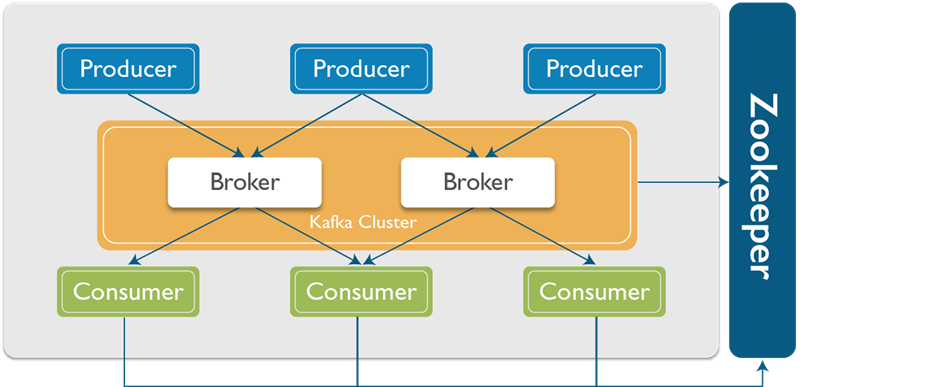
\includegraphics[width=0.8\textwidth]{Images/Kafka2.png}
    		\centering
    		\linebreak
    		\caption{Cấu trúc Kafka}
            \end{figure}
            
            \begin{itemize}
                \item Producer: Thành phần gửi message
                \item Message: Là message cần trao đổi đến các thành phần khác nhau trong hệ thống.
                \item Broker: Là tập hợp các server Kafka để lưu trữ các message
                \item Zookeeper: Được dùng để quản lý và bố trí các Broker
            \end{itemize}
            
            Tại sao lại sử dụng Kafka và không sử dụng Message Queue truyền thống
            
            Như nhóm đã trình bày ở phần trước thì Message Queue truyền thống sẽ đảm nhận nhiệm vụ xử lý bất đồng bộ trong từng service. Còn kafka sẽ là thành phần trung gian để gửi message từ service này đến service khác. Bởi vì kafka hoạt động rất nhanh do nó sử dụng cơ chế ZeroCopy, dữ liệu được sắp xếp theo khối, nén dữ liệu và giảm độ trễ I/O. Ngoài ra kafka rất dễ mở rộng khi lượng message cần trao đổi tăng lên và có cơ chế sao chép message ra nhiều partition để làm giảm rủi ro mất mát message trong quá trình xử lý.
		\end{itemize}
	
    \chapter{Bài toán và giải pháp}\label{chap:ProblemAndSolve}
		Sau khi phân tích, nghiên cứu các hệ thống và sản phẩm khác thì nhóm đã liệt kê ra một số bài toán cần phải giải quyết. Sau đây là phần trình bày của nhóm.
		
		\section{Bài toán xác thực user}
		Như chúng ta đã biết thì HTTP là 1 giao thức Stateless, nghĩa là khi Client gửi dữ liệu lên Server, Server thực thi xong và trả kết quả về cho Client thì quan hệ giữa Client và Server sẽ bị cắt đứt, Server sẽ không lưu lại bất cứ dữ liệu trạng thái gì của Client. Nói một cách dễ hiểu hơn là khi ta đăng nhập vào MyBK và sau đó di chuyển sang trang Thông tin Sinh viên thì chúng ta phải đăng nhập lại vì Server không lưu giữ bất kì thông tin gì của chúng ta. Để giải quyết vấn đề này thì Session/Cookies ra đời.
	
		\begin{figure}[H]
			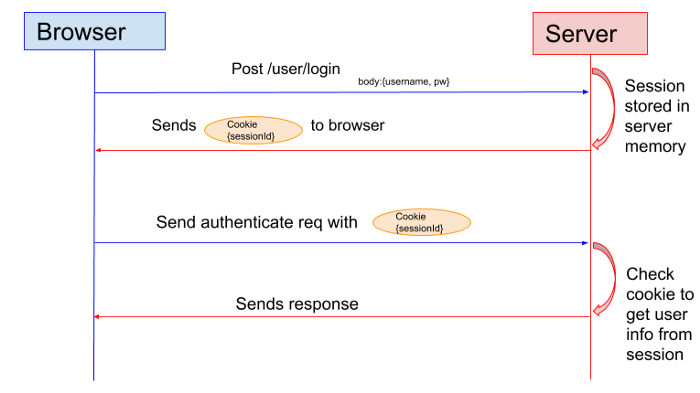
\includegraphics[width=0.8\textwidth]{Images/session-cookies.png}
			\centering
			\linebreak
			\caption{Xác thực dựa trên Session và Cookies}
		\end{figure}
		
		Đầu tiên user nhập thông tin tài khoản của mình. Sau khi kiểm tra đúng thông tin đăng nhập thì Server sẽ tạo ra 1 sessionID, lưu lại vào Database và trả về cho Client. Sau đó mỗi request gửi lên thì Client sẽ chèn sessionId vào Cookies và gửi lên cho Server từ đó Server kiểm tra và biết được chính xác Client đó là ai.\\
		
		Đối với hệ thống Micro Service thì việc xác thực theo cách này có 1 vấn đề đó là cần phải có 1 nơi để lưu trữ thông tin về session, ngoài ra cần phải xử lý các session đã hết hạn. Việc này có thể là giảm hiệu năng của 1 hệ thống Micro Service.\\
		
		Sau khi tìm hiểu thì nhóm sử dụng cơ chế xác thực dựa trên token. Với cơ chế như sau:
		
		\begin{figure}[H]
			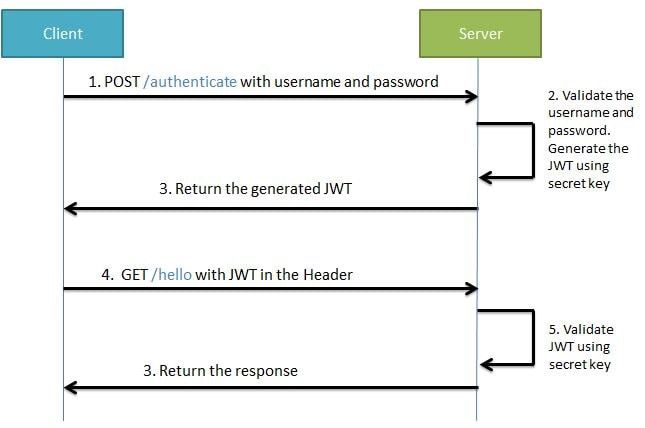
\includegraphics[width=1\textwidth]{Images/authbasedtoken.jpg}
			\centering
			\linebreak
			\caption{Xác thực dựa trên token}
		\end{figure}
		
		\begin{itemize}
                \item Client gửi thông tin đăng nhập lên Server
                \item Server xác thực thông tin đăng nhập. Nếu đúng sẽ tạo ra 1 token và gửi về cho Client
                \item Client đính kèm token mỗi khi request lên Server 
            \end{itemize}
		
		
		\section{Bài toán xác thực giữa các service}
		Do các service đươc deploy trên môi trường mạng vì thế có thể tiểm ẩn nhiều rủi ro bảo mật khi có sự giao tiếp giữa các service với nhau. Một kẻ tấn công nào đó có thể giả danh và gửi các request lên cho service của hệ thống xử lý. Do đó kẻ tấn công có thể lấy được các thông tin nhạy cảm của user (như số điện thọai, tên, địa chỉ, ngày tháng năm sinh, ...). Đây là một điều rất cấm kỵ khi chúng ta phải có nghĩa vụ bảo mật các thông tin nhạy cảm cho user.\\
		
		Sau khi tìm hiểu và so sánh các phương pháp thì nhóm sử dụng phương pháp tạo chữ ký số để xác thực request giữa các service với nhau. Khi service A muốn gọi service B thì service A phải có key của service B, Service A sẽ gửi thêm 1 trường thông tin là \textbf{sig = SHA256(data + key)}, service B khi nhận request thì sẽ tạo sig dựa vào key của mình và so sánh 2 sig đó có giống nhau không. Nếu giống thì mới tiếp tục thực hiện request của Service A, còn nếu không thì sẽ trả về lỗi cho service A.
		
		
		\section{Bài toán nhận nhiều Request của User}
		Thông thường 1 request của User sẽ được xử lý như sau: 
		
		    \begin{itemize}
                \item User gửi Request lên Server
                \item Server xử lý
                \item User nhận Response về từ Server 
            \end{itemize}
        
        Trong quá trình chờ Server xử lý thì User sẽ phải chờ đợi và nếu quá trình xử lý diễn ra lâu (bởi vì Server phải lưu thông tin vào database hay phải gọi Server khác,...) chính điều này sẽ ảnh hưởng đến trải nghiệm của User.\\
        
        Ngoài ra, trong những khoảng thời gian diễn ra các chương trình khuyến mãi giảm chi phí vận chuyển hoặc trong thời gian dịch bệnh thì nhu cầu vận chuyển hàng hóa để đáp ứng như cầu tiêu thụ của người dân. Do đó có thể trong 1 khoảng thời gian ngắn lượng Request đến hệ thống tăng cao. Nếu vẫn xử lý với cơ chế như bình thường thì hệ thống sẽ chết hoăc có thể không nhận đươc Request của User nữa. Điều này cũng ảnh hưởng nghiêm trọng đến trải nghiệm của User.\\
        
        Sau khi tìm hiểu và phân tích thì nhóm hiện thực chức năng tạo đơn hàng bằng cơ chế bất đồng bộ như sau:\\
        
        \begin{figure}[H]
			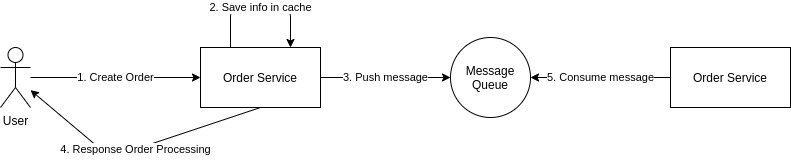
\includegraphics[width=1\textwidth]{Images/problem1.jpg}
			\centering
			\linebreak
			\caption{Quá trình tạo đơn hàng}
		\end{figure}
        
        Ở đây nhóm sử dụng MessageQueue(ActiveMQ) để hiện thực cơ chế bất đồng bộ. Sau khi user thực hiện tạo đơn hàng thì hệ thống sẽ lưu thông tin đơn hàng đó vào Cache, sau khi đã lưu thông tin đơn hàng vào Cache thì ta ngay lập tức phản hồi về cho User là đơn hàng đang được xử lý. Tiếp theo ta push message tạo đơn hàng đó vào MessageQueue, và sau đó đơn hàng sẽ được consume và tiếp tục xử lý.\\
        
        Việc sử dụng MessageQueue làm tách rời quá trình xử lý, Producer (service push message) chỉ cần đẩy message lên mà không cần quan tâm là message đó đã được xử lý hay không và Consumer (service consume message) chỉ cần lấy message và xử lý. Các mesage sẽ được lưu trữ trong Queue và chỉ mất đi khi đươc consume, điều này đảm bảo tất cả các message đề đươc xử lý duy nhất 1 lần và tất cả message sẽ không mất đi ngày cả khi OrderService bị chết do sự cố nào đó. Và đặc biệt lợi ích cuối cùng đó là trải nghiệm của User, User sẽ nhận phản hồi gần như lập tức sau khi tạo đơn hàng (mặc dù đơn hàng vẫn đang tiếp tục đươc xử lý) mà không cần phải chờ đợi các bước xử lý mất thời gian ở phía sau. 
	
		\section{Bài toán giảm thời gian xử lý khi User truy xuất thông tin}
		    Trong quá trình sử dụng ứng dụng thì việc lấy và hiện thị thông tin ra cho User diễn ra rất thường xuyên. Thông thường quá trình đó diễn ra như sau:
		    \begin{itemize}
                \item User gửi Request lấy thông tin lên Server
                \item Server truy xuất vào Database
                \item User nhận Response về từ Server 
            \end{itemize}
            
            
            Ở đây viêc truy xuất vào Database thường xuyên có thể làm giảm thời gian phản hồi do phải thực thi nhiều I/O operation. \\
            
            Vì thế, sau khi tìm hiểu và nghiên cứu thì nhóm sẽ sử dụng Cache để lưu lại các thông tin mà user thường xuyên truy xuất trong memory. Do thông tin được lưu trữ trong memory nên việc truy xuất và lấy các thông tin đó đươc thực hiện rất nhanh (gấp 500 lần so với thông tin lấy từ Database). Có rất nhiều chiến lược Cache có thể sử dụng nhưng nhóm sử dụng chiến lược Cache Aside để phù hợp với nhu cầu của ứng dụng:
            
            \begin{figure}[H]
			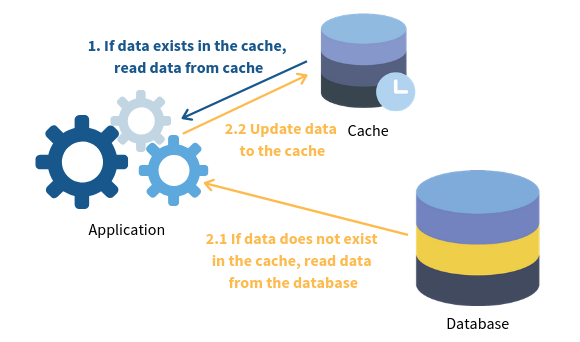
\includegraphics[width=1\textwidth]{Images/problem2.png}
			\centering
			\linebreak
			\caption{Chiến lươc Cache Aside}
	       	\end{figure}
	       	
	        Đầu tiên khi muốn lấy thông tin nào đó thì ta tiến hành tìm trong Cache. Nếu trong Cache có thông tin cần tìm kiếm thì lập tức trả thông tin đó về cho User, nếu không tìm thấy trong Cache thì ta tiến hành tìm kiếm trong Database, sau đó lưu thông tin đó vào Cache rồi mới trả về cho User.\\
	        
	        Việc sử dụng Cache đem lại hiệu quả nhưng cũng có 1 số điểm cần lưu ý như:
	         \begin{itemize}
                \item Thứ nhất là \textbf{Stale Cache}: Có nghĩa là dữ liệu trong Database và trong Cache không nhất quán với nhau dẫn đến trả về các thông tin cũ cho User. Nhóm giải quyết vấn đề này bằng cách mỗi khi cập nhật lại thông tin trong Database thì đều cập nhật luôn thông tin trong Cache. Việc này có thể làm tốn thêm nhiều chi phí nhưng nhóm chỉ lưu các thông tin mà User thường xuyên truy xuât nên chi phí sẽ giảm bớt và rất xứng đáng so với hiệu quả to lớn mà Cache mang lại.
                \item Thứ hai là \textbf{Invalidate Cache}: Có nghĩa là nếu để Cache quá lâu trong memory thì sẽ gây tiêu tốn dung lượng, còn nếu để Cache quá nhanh thì sẽ không có hiệu quả do cứ phải truy xuất Database nhiều. Trong quá trình tìm hiểu và thử nghiệm thì nhóm đã thiết lập thời gian tồn tại trong memory là 30 ngày. Là con số có thể chấp nhận đươc đối với mỗi đơn hàng mà User tạo ra.
            \end{itemize}
            
        
			
		\section{Bài toán xác định kho nguồn - kho đích ngắn nhất và tính chi phí vận chuyển}
			Để doanh nghiệp có thể tiết kiệm chí phí cũng như giảm được chí phí vận chuyển cho khách hàng thì bái toán xác định kho nguồn - kho đích so với địa chỉ của người gửi - người nhận sao cho ngắn nhất là một bài toán cần phải giải quyết sao cho tối ưu.\\\\
			\indent	Để xác định kho nguồn - kho đích ngắn nhất nhóm đã tìm quảng đường vận chuyển ngắn nhất giữa địa chỉ của người gửi so với tất cả địa chỉ của kho nguồn và giữa địa chỉ của người nhận so với tất cả địa chỉ của kho đích. Để xác định được quãng đường (km) nhóm đã sử dụng Google Map API để có thể tính đường quãng đường giữa hai địa chỉ cần xác định. Từ đó nhóm đã tìm được quãng đường tối ưu ngắn nhất và sử dụng tổng quãng đường vẫn chuyển ngắn nhất giữa hai địa chỉ người gửi - người nhận để tính toán chi phí cần vận chuyển đơn hàng cho người gửi. 
		\section{Bài toán thanh toán chi phí vận chuyển} 
		Thông thường để thanh toán chi phí vận chuyển thì người dùng sử dụng phương thức thu hộ (COD) hoặc thanh toán bằng tiền mặt khi nhận hàng, điều này gây ra nhiều bất tiện cho người dùng. Vì vậy, với xu hướng thanh toán không tiền mặt đang phát triển rộng rãi như hiện nay nên nhóm đẵ bắp kịp xu thế tích hợp cổng thanh toán online ZaloPay để người dùng có thể sử dụng thanh toán qua 3 hình thức thanh toán ví ZaloPay, Visa, Master, JCB (qua Cổng ZaloPay), thẻ ATM (qua Cổng ZaloPay).
		
		\begin{figure}[H]
			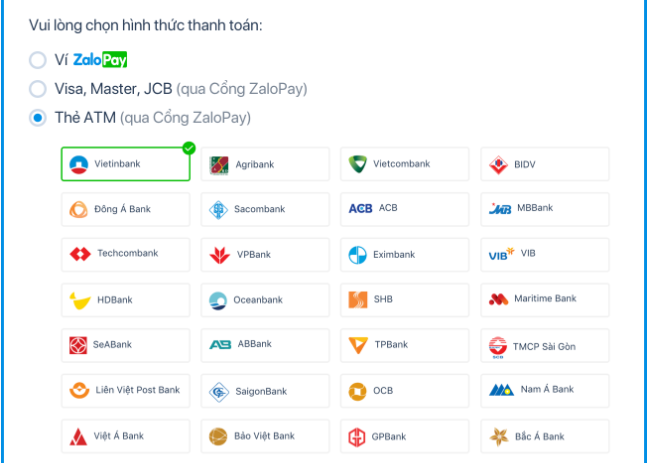
\includegraphics[width=0.6\textwidth]{Images/payment.png}
			\centering
			\linebreak
			\caption{Hình thức thanh toán}
		\end{figure}
		\section{Bài toán phân phối đơn hàng cho tài xế }
		    Trong các ứng dụng vận chuyển hàng thì bái toán phân phối là một bài toán rất hay, việc giải quyết bài toán này sao cho tối ưu có ảnh hưởng không nhỏ đến doanh thu của doanh nghiệp cũng như là chi phí của khách hàng.\\
		    
		    Ở hệ thống vận chuyển liên tỉnh mà nhóm đang làm thì sẽ có 3 giai đoạn phân phối: Đầu tiên là phân phối đơn hàng cho tài xế đi lấy, tiếp theo là phân phối đơn hàng cho tài xế liên tỉnh, cúôi cùng là phân phôi đơn hàng cho tài xế đi giao.
		    
		     \begin{itemize}
                \item \textbf{Phân phối đơn hàng cho tài xế đi lấy:} Sau khi đơn hàng được tạo ra bởi user thì sẽ có 2 cách để nhận hàng. Thứ nhất là user sẽ trưc tiếp đem hàng đến kho, thứ hai là hệ thống sẽ gán đơn đó cho tài xế và tài xế sẽ đi lấy hàng. Ở đây chúng ta nói về cách thứ hai. Sau khi đơn hàng được tạo ra thì hệ thống sẽ xác định được con đường ngắn nhất giữa 2 kho là kho nguồn và kho đích. Tài xế đi lấy sẽ là nhân viên ở kho nguồn. Hệ thống sẽ ngẫu nhiên thông báo cho một số tài xế ở kho nguồn là có đơn cần lấy. Tài xế nào đống ý nhận đơn trước thì sẽ được ưu tiên đi lấy hàng trước.\\
                
                Do hàng vận chuyển liên tỉnh, có thể số lượng sẽ rất lớn vì vậy nếu tài xế đầu tiên không lây hết thì hệ thống sẽ tự động thông báo cho các tài xế tiếp theo. Cứ như vậy đến khi hàng được lấy hết và chở về kho nguồn.\\
                
                Ở đây hệ thống sẽ thông báo cho một số tài xế của kho nguồn nhằm hạn chế việc tài xế được thông báo nhưng đang bận và chưa thể vận chuyển hàng về kho ngay lập tức được. Điều đó có thể làm chậm trễ thời gian giao vận mà user mong muốn gây ảnh hưởng đến trải nghiệm của user.
            
                \item \textbf{Phân phối đơn hàng cho tài xế  liên tỉnh:} Sau khi đơn hàng được vận chuyển đến kho nguồn thì việc tiếp theo hệ thống sẽ gán đơn hàng đó cho tài xế liên tỉnh để vận hàng hàng đến kho đích.\\
                
                Việc gán liên tỉnh sẽ được thực hiện vào 1 khung giờ cố định trong ngày (ví dụ: 19h mỗi ngày) và sẽ gán đơn hàng lên xe của 1 tài xế đến khi xe đầy thì chuyển sang xe của tài xế khác.\\
                
                Viêc gán vào 1 khung giờ cố định trong ngày nhằm để không làm giảm hiệu năng của hệ thống bời vì việc gán tài xế sẽ phải gọi service khác để lây thông tin và lưu database. Việc gán đơn hàng cho 1 xe đến khi đầy nhằm hạn chế tối đa chi phí bỏ ra để vận chuyển các đơn hàng đó. Nếu cùng 1 số lượng đơn hàng nhưng được gán lên rất nhiều xe để vận chuyển liên tỉnh thì sẽ tốn chi phí rất nhiều.
                
                \item \textbf{Phân phối đơn hàng cho tài xế  đi giao:} Sau khi đến kho đích thì đơn hàng tiếp tục được gán cho tài xế của kho đích đi giao. Việc gán đơn cho tài xế đi giao cũng được thực hiện vào 1 khung giờ cố định trong ngày và cách gán là lấy ra tất cả tải xế đi giao của kho đích và gán đều các đơn hàng cho tất cả tài xế. Việc gán này nhằm đảm bảo thời gian nhận hàng của người nhận là nhanh nhất có thể.
                
            \end{itemize}
            
            
            \section{Bài toán lưu trữ và truy xuất dữ liệu thống kê}
                Trong quá trình hoạt động và vận hành của hệ thống thì user thường xuyên xem lại những lịch sử mua hàng hay quản lý cần thống kê lượng tiền, lượng giao dịch xảy ra trong một khoảng thời gian nào đó.\\
                
                Thông thường chúng ta sẽ lưu hết vào Database rồi query SELECT COUNT(*) WHERE STARTDATE<=Date AND Date<=ENDDATE. Việc query như vậy vào Database sẽ được xử lý rất lâu cho nên sẽ làm giảm trải nghiệm của user.\\
                
                Sau khi tìm hiểu và nghiên cứu thì nhóm sử dụng cấu trúc dữ liệu \textbf{HyperLoglog} được hỗ trợ bởi Redis nhằm lưu trữ dữ liệu thống kế để mỗi khi cần chúng ta có thể truy xuất trong nháy mắt.\\
                
                \textbf{HyperLoglog} giúp chúng ta tính gần đúng các giá trị khác nhau trong tập hợp, thuật toán này có độ chính xác cao mà vẫn giữ được dung lượng dữ liệu rất bé, hỗ trợ nhiều thao tác liên quan tới việc đếm 1 phần tử trong 1 hoặc nhiều tập hợp. Và quan trọng nhất là nó rất nhanh nêu chúng ta tổ chức dữ liệu một cách hợp lý.\\
                
                \begin{figure}[H]
			    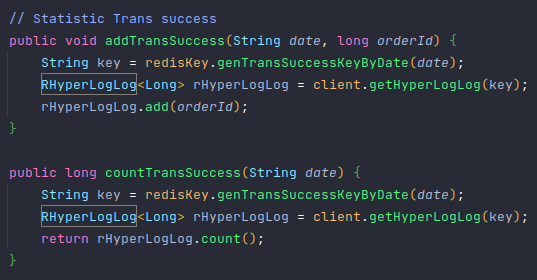
\includegraphics[width=1\textwidth]{Images/hyperloglog.png}
			    \centering
			    \linebreak
			    \caption{Ví dụ về HyperLoglog}
	       	    \end{figure}
	       	
	       	    Trong đoạn code trên ta lưu thông tin của số giao dịch thành công trong 1 ngày. Khi có yêu cầu lấy thông tin về số giao dịch thành công trong một khoảng thời gian nào đó thì ta chỉ cần gọi hàm như ví dụ để lấy. Do các thông tin này được lưu trên memory nên việc xử lý rất nhanh đảm bảo trải nghiệm tốt cho user.
		  
		  \section{Bài toán triển khai các services và cơ sở hạ tầng}
		 
		  
		  Việc deploy hệ thống có thể được hỗ trợ bởi rất nhiều bên như: Git, Heroku, ... thông thường chúng ta chỉ đưa mã nguồn lên Git, thiết lập một vài bước là có thể dễ dàng triển khai hệ thống lên cho khách hàng sử dụng. Nhưng do nhóm sử dụng khá nhiều hạ tầng liên quan để tăng cường hiệu suất cho hệ thống như: Redis, Kafka, Mysql, Message Queue, Cassandra, ...cho nên việc sử dụng các nền tảng đó sẽ không được hỗ trợ một cách tối đa. Ngoài ra để hiểu rõ hơn về quy trình deploy một ứng dụng cũng như là cơ hội để có thể áp dụng các kiến thức đã được học về Network, System, Security, ... vào thực tế thì nhóm quyết định thuê 1 VPS (Virtual Private Server) trên Google Cloud Platform để tự cấu hình và triển khai hệ thống của mình.\\
		  
		  Như đã trình bày ở phần Công nghệ để deploy nhanh chóng, tiện lợi các services và cơ sở hạ tầng đi kèm thì nhóm sử dụng nền tảng \textbf{Docker} và \textbf{Docker compose}.
		  
		  
		  \begin{figure}[H]
		  	\centering
		  	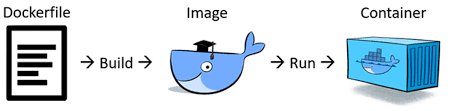
\includegraphics[width=0.8\linewidth]{Images/flowDocker}
		  	\linebreak
		  	\caption{Flow docker}
		  \end{figure}
		  
		  Đầu tiên thì mỗi service cần phải có một \textbf{Dockerfile}, sau đó tiến hàng build Dockerfile thì ta có được \textbf{Image}, cuối cùng chỉ cần chạy Image đó là ta đã deploy được service trong \textbf{Container}.
		  
		  \begin{figure}[H]
		  	\centering
		  	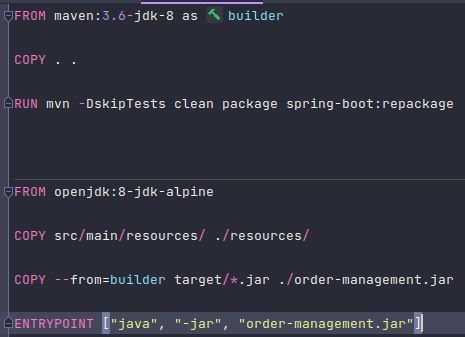
\includegraphics[width=0.7\linewidth]{Images/DockerfileOrderService}
		  	\linebreak
		  	\caption{Dockerfile OrderService}
		  \end{figure}
		  
		  Dockerfile thực thi các câu lệnh để build ra file *.jar và chạy file jar đó trong containers. Ở đây thì nhóm có tìm hiểu một số kỹ thuật để tăng cường hiệu suất cho Docker như sau:
		  
		  \begin{itemize}
		  	\item \textbf{Multi-stage build}: Thông thường để chạy được service ta cần phải tạo môi trường, cấu hình package, module, ... và sẽ cần dung lượng khá cao, làm cho Image nặng lên từ đó làm tăng thời gian build, run và làm giảm hiệu suất của Docker. Vì thể nhóm sẽ build Image trên 2 stage, ở stage thứ nhất thì ta thiết lập môi trường, các package liên quan sau đó tiến hành build file *.jar. Ở stage thứ 2 ta chỉ cần copy file *.jar qua và thực thi. Điều này giúp cho quá trình build và run Image trở nên nhanh hơn đáng kể.
		  	\item \textbf{Sử dụng base image đươc dựng trên alpine}: Alpine Linux là một distro linux dựa trên musl và busybox, được phát triển chú trọng về đơn giản, bảo mật và hiệu quả tài nguyên. Ở đây nhóm đã sử dụng base image đó là: openjdk:8-jdk-alpine để thực thi file *.jar.
		  \end{itemize}
		  
		  
		  Một hệ thống thông thường sẽ phải deploy rất nhiều container khác nhau. Khi có nhiều container việc phải start, stop, run từng container trở nên khó khăn và khó quản lý. Vì thế nhóm đã dụng \textbf{Docker compose} cho phép quản lý nhiều container một cách rất dễ dàng.\\
		  
		  Tương tự như các service thì các cơ sở hạ tầng như: MySQL, Cassandra, Redis, Kafka, ActiveMq, ... cũng được deploy và triển khai dựa trên Docker.
		  
		  \begin{figure}
		  	\centering
		  	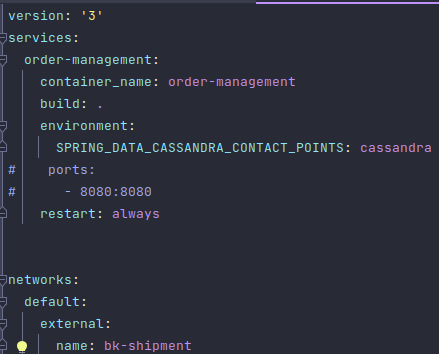
\includegraphics[width=0.8\linewidth]{Images/DockercomposeOrderService}
		  	\linebreak
		  	\caption{Docker compose OrderService}
		  \end{figure}
		  
		  \begin{figure}
		  	\centering
		  	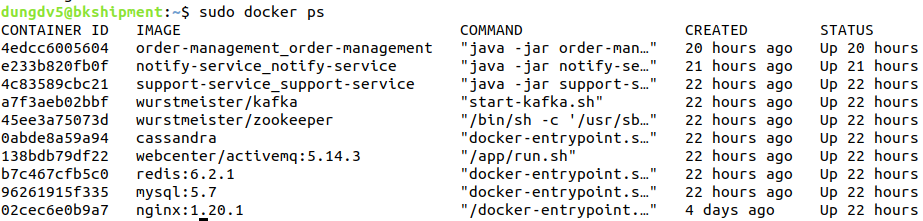
\includegraphics[width=0.8\linewidth]{Images/DockerResult}
		  	\linebreak
		  	\caption{Kết quả}
		  \end{figure}
	  
	  \newpage
	  
	  \section{Bài toán bảo mật các service trong private network, cấu hình SSL, cân bằng tải}
	  
	  Thông thường sau khi deploy thì các service được gọi thống qua \textbf{IP:port/service-name/...}, điều này có nghĩa là service sẽ được public ra bên ngoài. Điều này có thê gặp một số rủi ro về vấn đề an ninh và bảo mật. Vì thế nhóm đã sử dụng NGINX như là một \textbf{Reverse Proxy} để tăng cường bảo mật, cũng như cân bằng tải.\\ 
	  
	  
	  \begin{figure}[H]
	  	\centering
	  	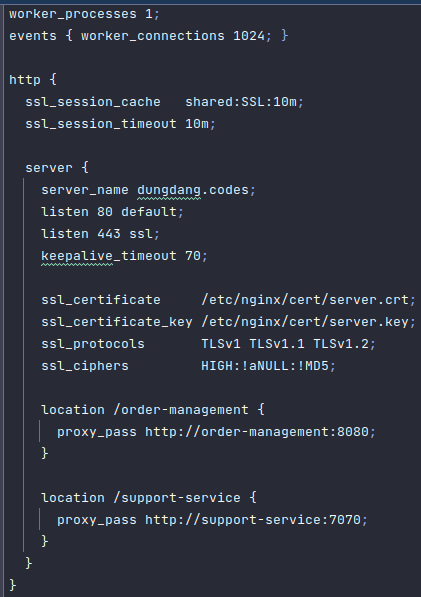
\includegraphics[width=0.7\linewidth]{Images/NGINXconfig}
	  	\linebreak
	  	\caption{Cấu hình của NGINX}
	  \end{figure}
  	
		Như trên file đã cấu hình thì server Frond end có thể gửi request xuống server Back end thông qua domain là: \textbf{dungdang.codes} ở port 80 cho HTTP và 443 cho HTTPS. Đối với những request có domain là: https://dungdang.codes/order-management/... sẽ được route vào service đươc deploy ở port 8080 còn https://dungdang.codes/support-service/... thì sẽ được route vào service deploy ở port 7070. Điều này đã giúp che giấu và bảo mật các services chạy trong private network.
		
		  \section{Bài toán gợi ý địa điểm khi người dùng nhập địa chỉ}
		  
		  Khi điền địa chỉ muốn gửi trong giao diện tạo đơn hàng, hệ thống sẽ tự động gợi ý địa điểm cho người dùng khi người dùng nhập vài từ trong địa chỉ. Điều này được thực hiện nhờ sử dụng API \textbf{Places Autocomplete} mà Google cung cấp. Cụ thể, nhóm đã đăng ký một tài khoản trên Google Cloud Platform, kích hoạt dịch vụ \textbf{Maps JavaScript API} và tiếp tục làm theo hướng dẫn để lấy được một api key giúp cho ta có thể gọi và sử dụng api của Google. Việc sau đó là chỉ cần gọi API trên ở phía client-side code. Ví dụ cho việc gợi ý địa điểm trong ứng dụng như sau:
		  
		  \begin{figure}[H]
		  	\centering
		  	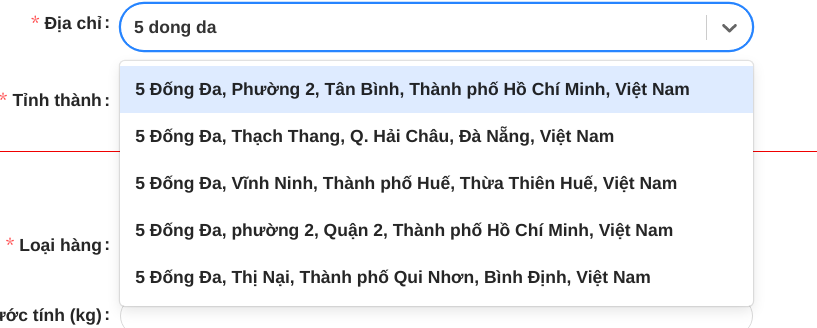
\includegraphics[width=1\linewidth]{Images/FE_Problems/places_autocomplete}
		  	\linebreak
		  	\caption{Giao diện gợi ý địa điểm khi người dùng nhập địa chỉ}
		  \end{figure}
		
			Từ địa chỉ gợi ý mà người dùng chọn, nhóm có thể xác định được thành phố người dùng muốn gửi đến là ở đâu để từ đó tiếp tục thực hiện quy trình vận chuyển liên tỉnh.
			
			\section{Bài toán giảm thời gian load trang web lần đầu tiên}
			
			Như đã trình bày ở phần công nghệ, nhóm sử dụng dịch vụ của gitlab pages để host và serve các static files (HTML, CSS, JS, image vv...) khi người dùng truy cập vào tên miền của trang web. Tuy vậy, gitlab pages không tự động compress (nén) các static files theo định dạng gzip cho người dùng. Chính vì thế nhóm đã tự nén các file lại theo định dạng gzip khi build code để giúp tiết kiệm băng thông cũng như giúp thời gian load trang web trở nên nhanh hơn khi người dùng truy cập.\\
			
			Cơ chế hoạt động cơ bản của gzip trong giao tiếp giữa máy khách và máy chủ:
			\begin{itemize}
				\item Bước 1: Trình duyệt gửi một header request đến server (máy chủ) để thông báo rằng nó chấp nhận file được nén. Header này sẽ có dạng như sau: \textbf{Accept-Encoding: gzip}.
				\item Bước 2: Server gửi phản hồi đồng ý và truyền file dữ liệu đã được nén cho trình duyệt với tín hiệu: \textbf{Content-Encoding: gzip}
			\end{itemize}
			
    \chapter{Phân tích và thiết kế hệ thống}

\section{Phân tích yêu cầu}
    \subsection{Yêu cầu người dùng}
    	\begin{itemize}
				\item \textbf{Đối với người dùng}
					\begin{itemize}
				        \item \textbf{Đăng kí, đăng nhập đổi mật khẩu} cho người dùng.
				        \item \textbf{Chỉnh sửa thông tin cá nhân}: Người dùng có thể dễ dàng thay đổi thông tin cá nhân của mình.
				        \item \textbf{Tạo đơn hàng}: Lúc tạo đơn hàng người dùng có thể tự đến gửi hàng trực tiếp tại kho hoặc người dùng lựa chọn có tài xế đến lấy, phí vận chuyển có thể là người gửi thanh toán hoặc người nhận thanh toán.
				        \item \textbf{Hủy đơn hàng}: Trong khoảng thời gian đơn hàng được xác nhận bởi tài xế thì đơn hàng có thể bị hủy. Chú ý rằng sau khi đơn hàng đã được xác nhận thì người dùng không thể hủy.
				        \item \textbf{Xem danh sách các đơn hàng}: Người dùng có thể dễ dàng xem thông tin đơn hàng. Danh sách đơn hàng có thể được lọc theo trạng thái, theo mã đơn hàng hoặc theo từng khoảng thời gian khác nhau nhanh chóng.
				        \item \textbf{Xem nợ công và thanh toán}: Người dùng có thể xem các đơn hàng đã hoàn tất và tiến hành thanh toán trung gian qua Ví điện tử hoăc thẻ ngân hàng.

				        \item \textbf{Nhận thông báo}: Sau khi đơn hàng được xác nhận bởi tài xế, thì ngươi dùng sẽ liên tục nhận được thông báo mỗi khi chuyển trạng thái của đơn hàng. Điều này giúp cho người dùng có thể theo dõi đơn hàng chặt chẽ và dễ dàng dự báo thời gian nhận hàng của mình.

				        \item \textbf{Tìm kiếm đơn hàng}: Đối với người nhận không phải là người dùng của hệ thống thì vẫn có thể dễ dàng xem thông tin các đơn hàng thông qua số điện thoại của mình hoặc theo dõi yêu cầu thông qua mã yêu cầu.
				        \item \textbf{Yêu cầu hỗ trợ}: Khi có các vấn đề thắc mắc thì người dùng có thể gửi yêu cầu để quản lý trực tiếp phản hồi. Danh sách các yêu cầu có thể được lọc theo mã yêu cầu, ngày, tháng, năm.
				        
				    \end{itemize}
				
			         
				\item \textbf{Đối với tài xế}
	                \begin{itemize}
	                    \item \textbf{Chỉnh sửa thông tin cá nhân}: Tài xế có thể dễ dàng thay đổi thông tin cá nhân của mình.
	                    \item \textbf{Nhận đơn hàng}: Sau khi đơn hàng được tạo ra thì tài xế có thể nhận đơn và tiến hành vận chuyển hàng hóa.
	                    \item \textbf{Xem danh sách kiện hàng cần lấy}: Hệ thống sẽ tự động gán đơn đối với tài xế liên tỉnh và tài xế đi giao cho nên tài xế cần theo dõi danh sách đơn hàng cần lấy để lấy đúng kiện hàng mà mình vận chuyển.
	                    \item \textbf{Xem danh sách kiện hàng cần giao}: Tài xế có thể xem thông tin chi tiết về các đơn hàng mà mình cần giao.
	                    \item \textbf{Xác nhận đơn hàng với người dùng}: Trong quá trình giao nhận hàng giữa tài xế và người dùng (người nhận, người gửi) thì tài xế đều phải xác nhận đơn hàng.
	                    \item \textbf{Báo cáo vấn đề}: Trong quá trình vận chuyển có thể xảy ra các vấn đề ngoài ý muốn như: làm thất lạc hàng, gặp sự cố ngoài ý muốn không thể đảm bảo thời gian giao hàng,... thì tài xế có thể báo cáo lên để quản lý có thể giải quyết.
	                    \item \textbf{Nhận thông báo}: Mỗi khi đơn hàng được gán cho tài xế thì sẽ có mail thông báo cho tài xế. Việc nay giúp tài xế nắm thông tin đơn hàng, đảm bảo việc giao nhận diễn ra kịp thời.
	                \end{itemize}
	                
	                
				\item \textbf{Đối với thủ kho}
			    	\begin{itemize}
			    	    \item \textbf{Chỉnh sửa thông tin cá nhân} thủ kho.
	                    \item \textbf{Nhập kho}: Sau khi đơn hàng vận chuyển đến kho thì thủ kho có trách nhiệm xác nhận đơn hàng đúng về số lượng và đảm bảo chất lượng nguyên vẹn. Sau khi xác nhận thì tiến hành nhập kho để lưu trữ và phân phối tiếp tục cho tài xế.
	                    \item \textbf{Xuất kho}: Sau khi đơn hàng đã phân phối cho tài xế thì thủ kho có trách nhiệm kiểm tra hàng một lần nữa và bàn giao cho tài xế. 
	                    \item \textbf{Xuất hóa đơn}: Trong quá trình nhập kho và xuất kho thì thủ kho có thể xuất hóa đơn để xác nhận đã nhập hàng hoặc bàn giao hàng hóa cho tài xế.
	                    \item \textbf{Xem danh sách đơn hàng}: Thủ kho có thể xem danh sách đơn hàng đang ở trong kho mà mình quản lý. Danh sách đơn hàng được lọc theo mã hoặc có thể theo ngày, tháng, năm.
	                    \item \textbf{Xem lịch sử nhập xuất}: Thủ kho có thể xem lịch sử nhập xuất đơn hàng vào/ra kho.
	                \end{itemize}
	                
	                
				\item \textbf{Đối với quản lý}
				    \begin{itemize}
	                    \item \textbf{Tạo tài khoản cho tài xế}: Quản lý có thể tạo tài khoản và phân kho cho tài xế khi tài xế mới nhận việc.
	                    \item \textbf{Xem biểu đồ thống kê}: Quản lý có thể xem biểu đồ thống kê về tình hình hoạt động của các kho, tình hình vận chuyển hàng hóa.
	                    \item \textbf{Xem thông tin} các tài xế, thủ kho và kho tương ứng của hệ thống.
	                    \item \textbf{Xử lý sự cố}: Khi nhận được sự cố từ tài xế thì quản lý có thể xử lý sự cố và cập nhật trạng thái đơn hàng cho người dùng.
	                    \item \textbf{Xử lý yêu cầu từ người dùng}: Khi người dùng yêu cầu thì quản lý có thể phản hồi thắc mắc hoặc các phản ánh từ người dùng.
	                \end{itemize}
		\end{itemize}
    
    \subsection{Yêu cầu hệ thống}
    Hệ thống vận chuyển hàng hóa liên tỉnh cần đáp ứng một số yêu cầu về hệ thống như sau:
        \begin{itemize}
            \item Thời gian xử lý mỗi request từ người dùng không quá 1 giây.
            \item Hệ thống gửi thông báo cho người dùng hoặc tài xế  không quá 5 giây.
            \item Hệ thống có thể chịu tải 100 yêu cầu mỗi giây.
            \item Thời gian tải hóa đơn nhập hàng/xuất hàng không quá 2 giây.
            \item Hệ thống cần mã hóa thông tin giao tiếp giữa máy khách và máy chủ.
            \item Hệ thống phải được thiết kế để khi có nhu cầu mở rộng, thêm tính năng mới phải dễ dàng.
            \item Hệ thống cần xuất thống kê về số lượng đơn hàng được vận chuyển thành công, thất bại, doanh thu vào ngày cuối cùng trong tháng.
        \end{itemize}
    
    \newpage

\section{Thiết kế hệ thống}

\subsection{Kiến trúc hệ thống}
	
		\begin{figure}[H]
			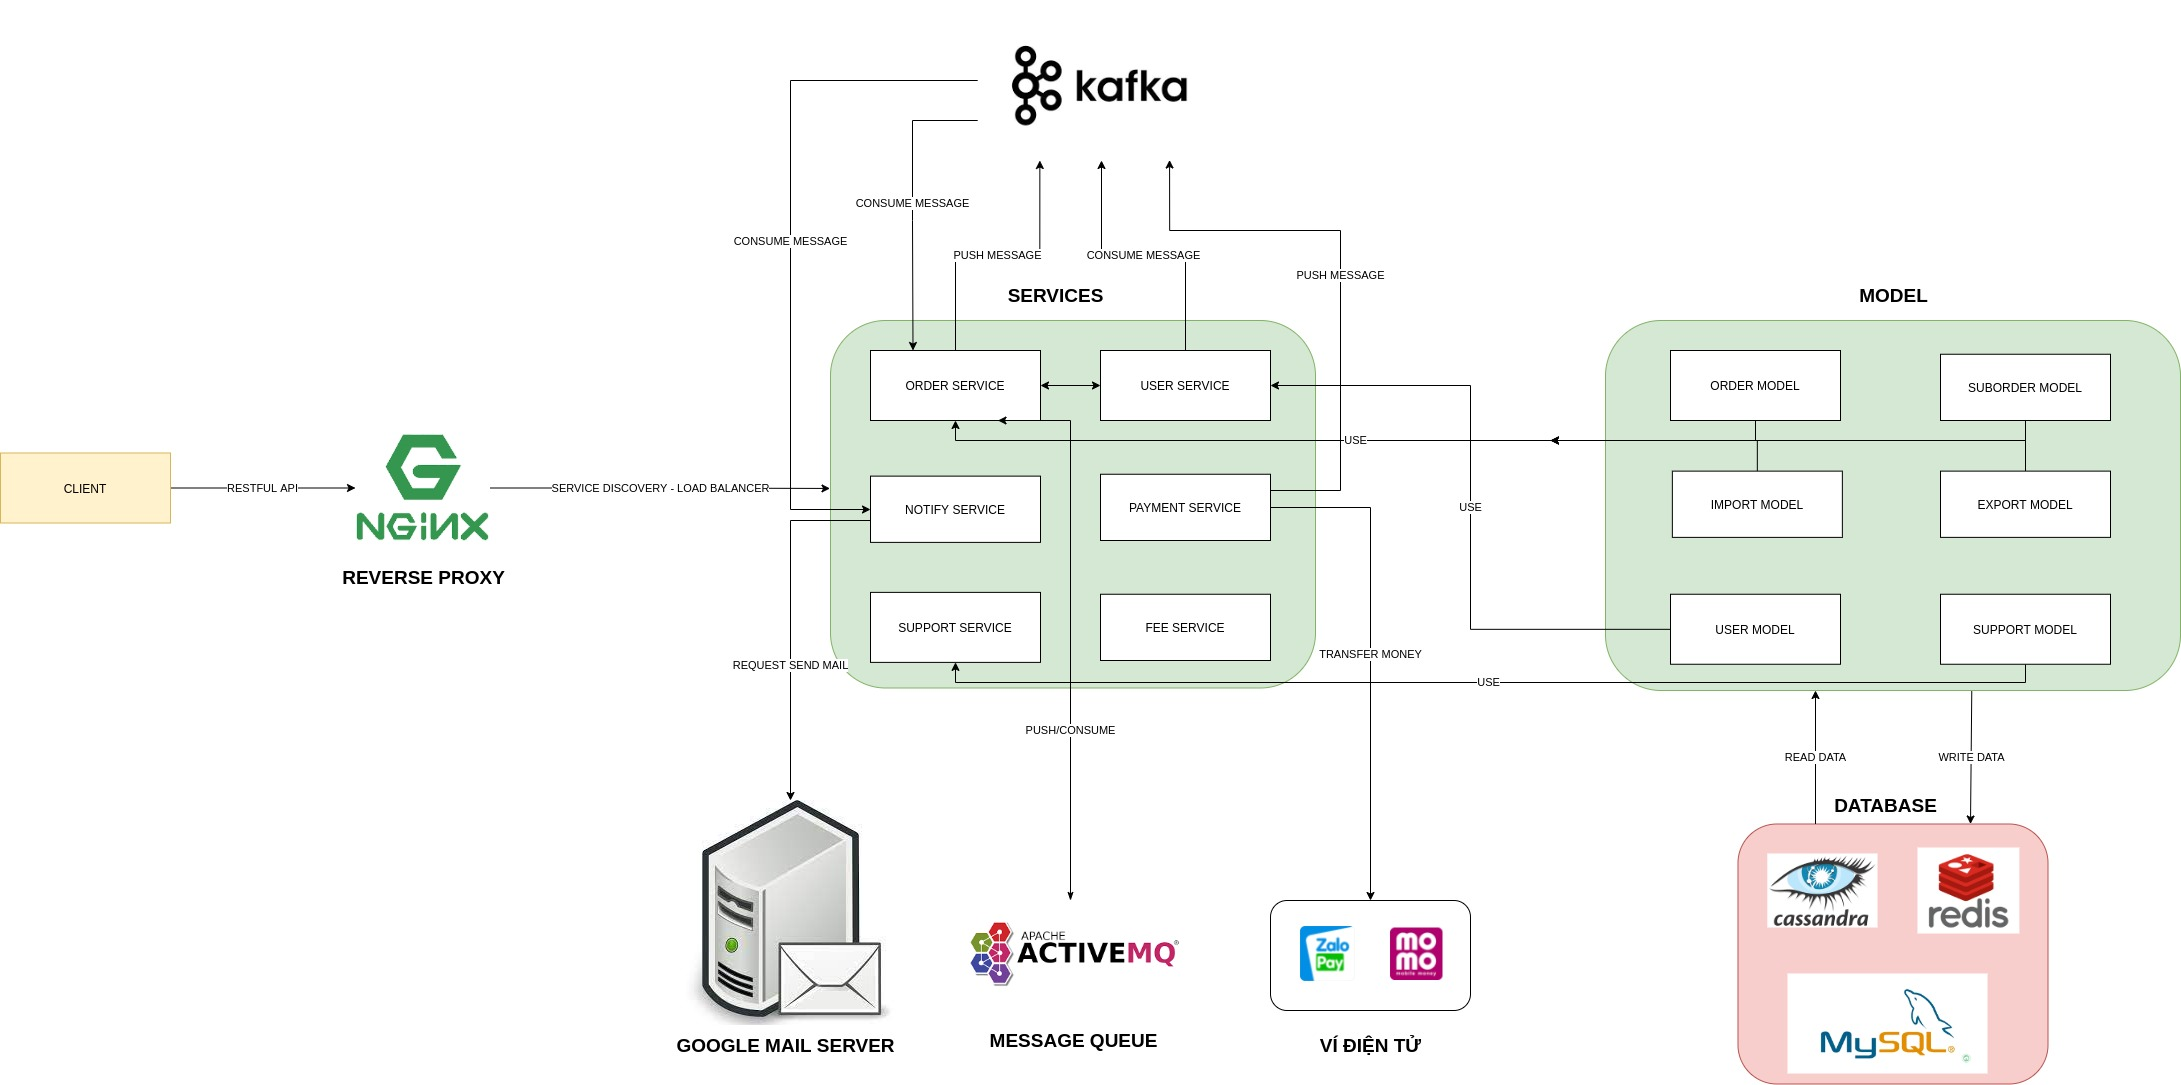
\includegraphics[width=1\textwidth]{Images/SystemArchitecture.jpg}
			\centering
			\linebreak
			\caption{Kiến trúc hệ thống}
		\end{figure}
	

		
		\begin{itemize}
			\item \textbf{User Service}
			\begin{itemize}
				\item Service chịu trách nhiệm quản lý user trong hệ thống. Ở đây sẽ lưu trữ Database của user.
				\item Mỗi khi user login vào hệ thống thì sẽ vào Service này để authen: Ban đầu user được yêu cầu sẽ nhập username và password, Sau khi authen là đúng user đó thì hệ thống sẽ sinh ra JWT (Json Web Token) để gửi trả về cho user. Sau này cứ mỗi request lên hệ thống thì user sẽ gửi kèm theo JWT để hệ thống có thể authen và author.
				\item User có thể get thông tin để có thể xem và chỉnh sửa
			\end{itemize}
			\item \textbf{Order Service}
			\begin{itemize}
				\item Service chịu trách nhiệm tạo, xử lý, lưu trữ các thông tin về đơn hàng cho người dùng.
				\item Ngoài ra service còn chịu trách nhiệm phân phối các đơn hàng đến tài xế
				\item Đây là service chịu tải khá lớn trong hệ thống vì nhóm sử dụng kết hợp các giải pháp sau nhằm tăng hiệu suất cho service: 
					\begin{itemize}
						\item Sử dụng Message Queue để hiện thực cơ chế bất đồng bộ cho các tác vụ: Tạo đơn hàng, ghi dữ liệu vào Database.
						\item Sử dụng Kafka để gửi message cho service khác
						\item Trong quá trinh xử lý thì dữ liệu của đơn hàng được lưu trên Cache. Đến khi nào có \textbf{trạng thái cuối} thì đơn hàng mới được lưu vào Database. Bởi vì đơn hàng đươc lấy và thay đổi trạng thái rất nhiều lần trong quá trình xử lý, nếu ghi vào Database (thực hiện nhiều I/O operations) sau mỗi lần xử lý như vậy thì sẽ làm giảm hiệu năng của hệ thống rất nhiều. Việc xử lý dữ liệu trên Cache cũng có thể gặp rủi ro như Cache Server sập thì dữ liệu có thể mất hết, nhưng rất may Redis có hỗ trợ cơ chế Persistence (định kỳ sao lưu dữ liệu) nên rủi ro này có thể chấp nhận được.
					\end{itemize}
				\item Mỗi khi đơn hàng thay đổi trạng thái hoăc tài xế đươc phân phối đơn thì service sẽ produce message vào \textbf{Kafka Broker} để \textbf{Notify Service} consume và tiếp tục xử lý
			\end{itemize}
			\item \textbf{Notify Service}
			\begin{itemize}
				\item Service chịu trách nhiệm quản lý các thông báo cho hệ thống.
				\item Service sẽ consume message tử \textbf{Order Service} và gửi yêu cầu về mail cho \textbf{Google Mail Server}.
				\item Hệ thống sẽ gửi thông báo mỗi khi: 
					\begin{itemize}
						\item Gửi thông báo cho khách hàng mỗi khi trạng thái đơn hàng thay đổi. 
						\item Gửi thông báo cho tài xế mỗi khi được phân phối đơn.
						\item Gửi mã xác thực OTP
					\end{itemize}
			\end{itemize}
			\item \textbf{Fee Service}
			\begin{itemize}
				\item Service chịu trách nhiệm hiện thực giải thuật, công thức để tính toán các khoản phí phát sinh cho khách hàng.
				\item Database lưu thông tin về phí của mỗi đơn hàng để người dùng có thể đối soát.
			\end{itemize}
			\item \textbf{Payment Service}
			\begin{itemize}
				\item Service này sẽ liên kết với 1 bên thứ 3 như: ngân hàng, ví điện từ, .... để thực hiện chức năng thanh toán cho người dùng.
			\end{itemize}
			\item \textbf{Reverse Proxy}
			\begin{itemize}
				\item Hệ thống sử dụng NGINX như là một \textbf{Reverse Proxy} nhằm thực hiện một số chức năng như: 
				\begin{itemize}
					\item \textbf{Bảo mât}: Kiểm soát các yêu cầu của Client gửi tới, nếu hợp lệ sẽ luân chuyển đến các service bên trong để xử lý. Che giấu địa chỉ IP của các service bên trong nhằm giúp các service trách khỏi các cuôc tấn công mạng. Ngoài ra còn có thể dễ dàng thiết lập SSL nhằm mã hóa dữ liệu trong quá trình giao tiếp giữa Client và các service bên trong.
					\item \textbf{Cân bằng tải}: Mỗi service có thể được deploy với nhiều instance để có thể chịu tải cao hơn. Reverse proxy sẽ thực hiện một số giải thuật như: Round Robin, Least Connection, ... để đẩy các request vào cho các service xử lý.
				\end{itemize}
			\end{itemize}
			
				\item \textbf{Database}
				\begin{itemize}
					\item \textbf{MySQL}: Hệ thống sử dụng MySql để lưu các thông tin ít được truy xuất như log, cấu hình service,...
					\item \textbf{Cassandra}: Với khả năng đọc/ghi có tốc độ nhanh cùng với đó là khả năng chịu lỗi cao hệ thống sử dụng Cassandra để lưu các thông tin về Order, Hóa đơn nhập/xuất kho,...
					\item \textbf{Redis}: Với Redis thì dữ liệu được lưu trữ trong memory vì thế giúp cho service truy xuất thông tin rất nhanh chóng. Hệ thống sẽ lưu các thông tin thường xuyên được truy xuất bởi người dùng như thông tin về yêu cầu, đơn hàng,... Ngoài ra còn tận dụng cấu trúc dữ liệu đa dạng trong Redis để giải quyết một số bài toán phức tạp. 
				\end{itemize}
		
		\end{itemize}

\newpage
\subsection{Thiết kế và đặc tả Use Case}

\begin{figure}[H]
	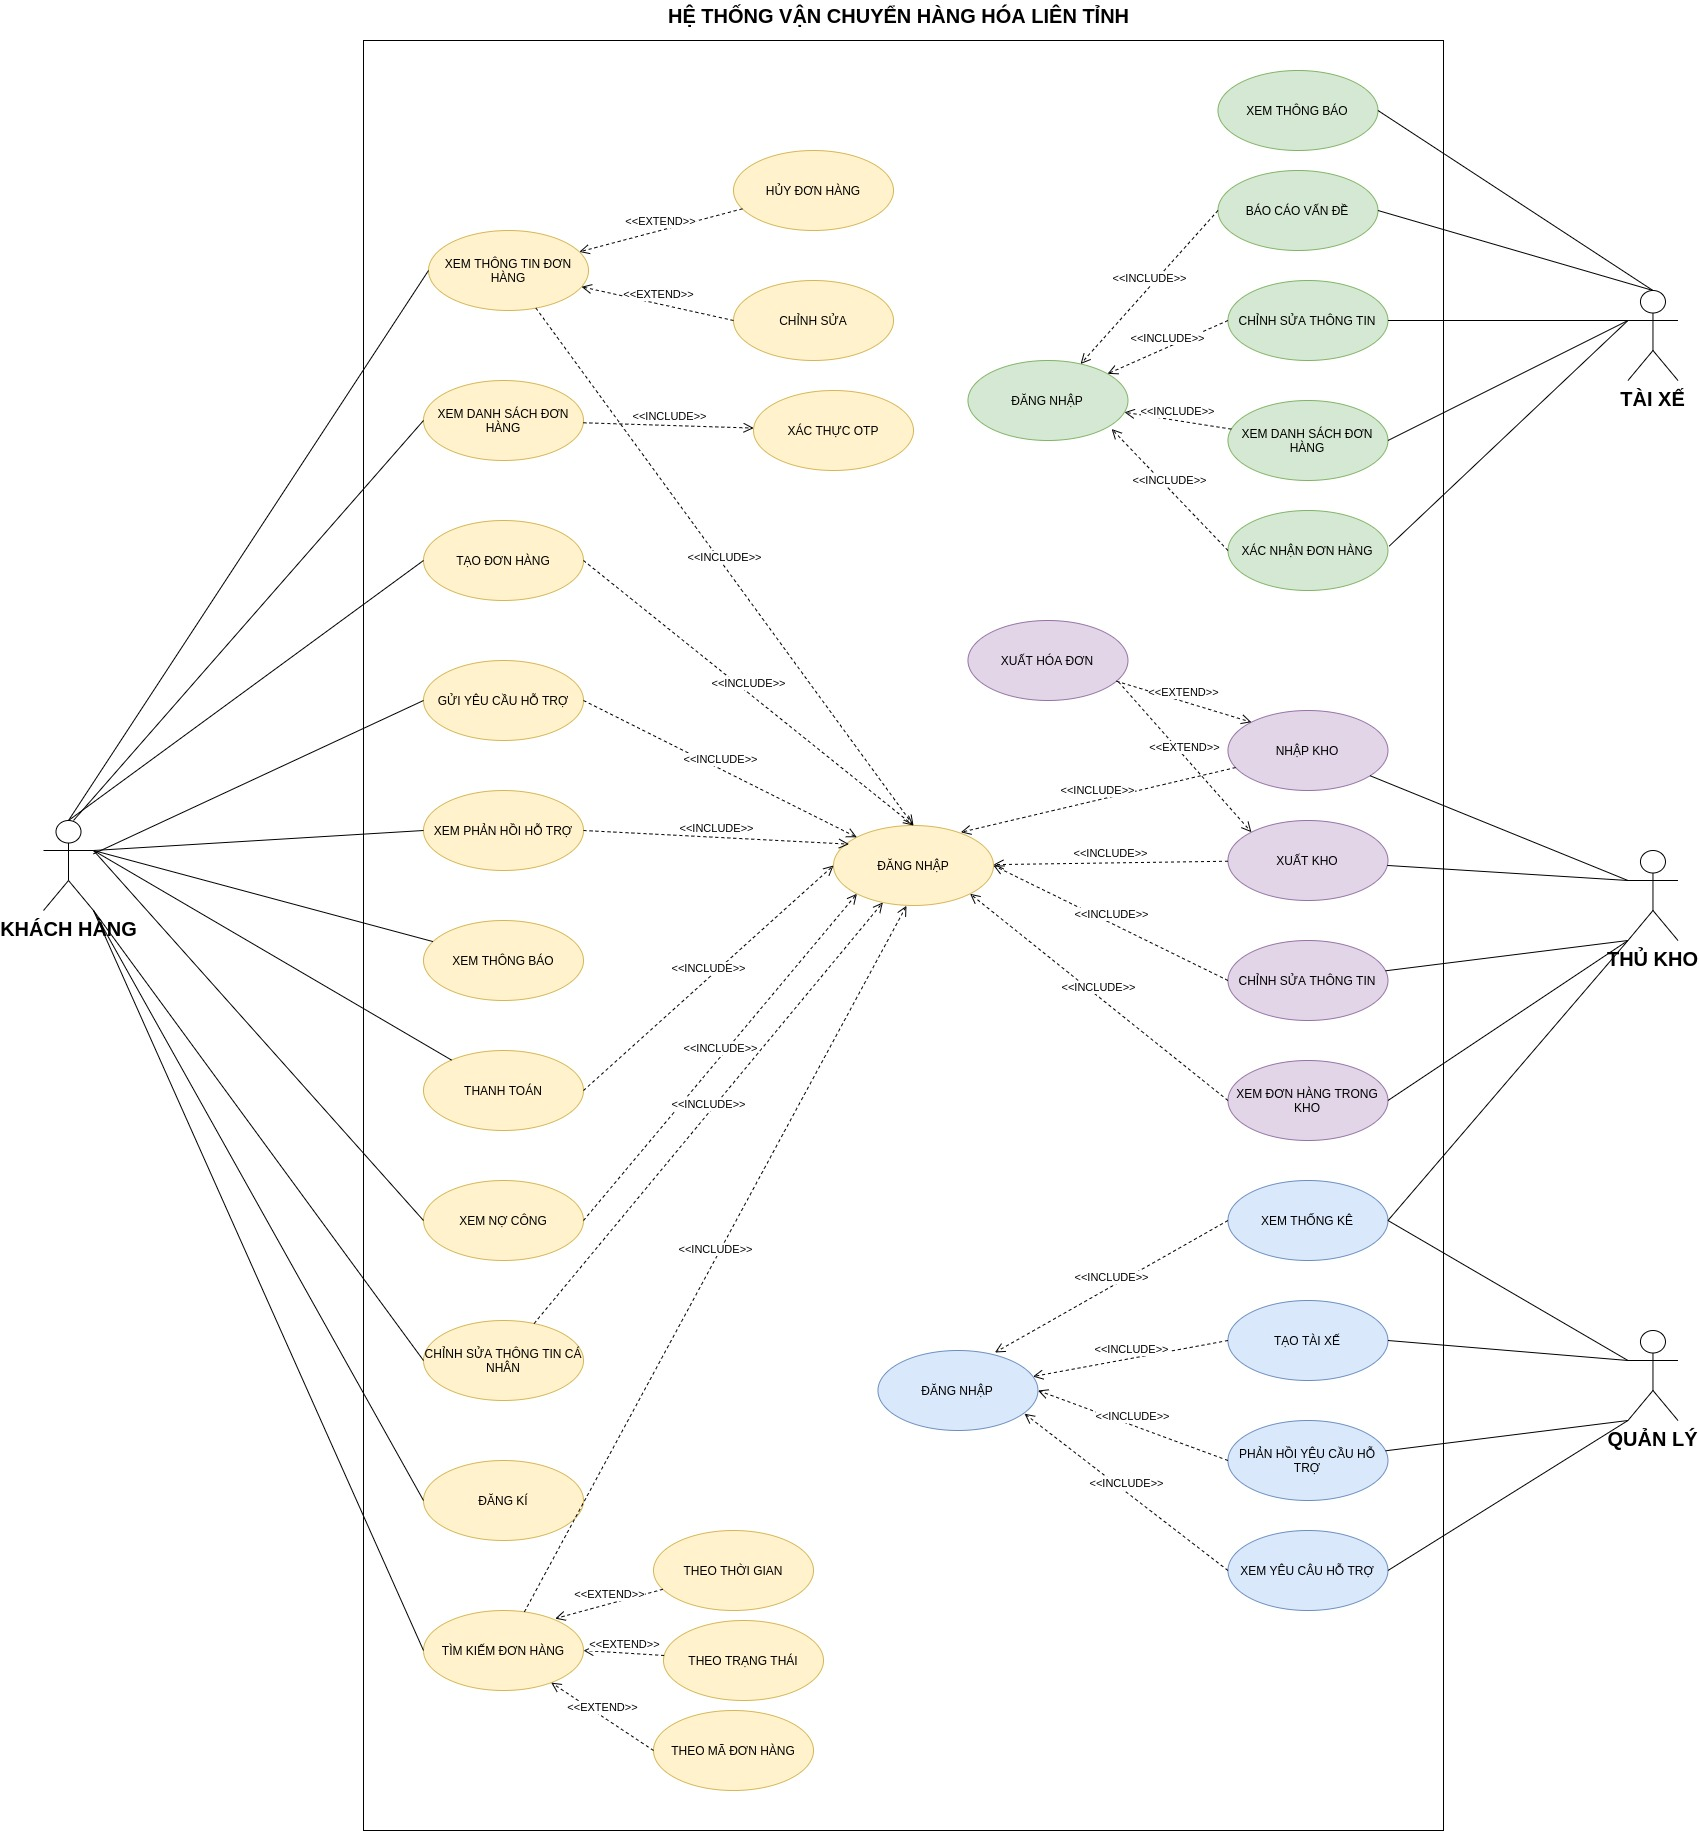
\includegraphics[width=1\textwidth]{/UseCase.jpg}
	\centering
	\linebreak
	\caption{Sơ đồ Use case}
\end{figure}

	\newpage
	
	\begin{itemize}
		\item \textbf{Use case cho Khách Hàng}
		\begin{itemize}
			\item \textbf{Tạo đơn hàng:} Người gửi cần điền những thông tin sau: 
			\begin{itemize}
				\item Bên gửi: Hệ thống sẽ tự động nhập thông tin khi người gửi đăng nhập bao gồm:
				\begin{itemize}
					\item Tên người gửi
					\item Số điện thoại
					\item Địa chỉ, chia làm 4 phần gồm Số địa chỉ + tên đường, Phường - Xã, Quận - Huyện, Thành phố - Tỉnh. 
				\end{itemize}
				\item Bên nhận:
				\begin{itemize}
					\item Tên người nhận
					\item Số điện thoại
					\item Địa chỉ, tương tự như bên gửi. Khi người gửi nhập địa chỉ hệ thống sẽ tự động lấy chính xác địa chỉ thông qua Google Map API.
				\end{itemize}
				\item Thông tin về món hàng muốn gửi:
				\begin{itemize}
					\item Loại hàng hóa
					\item Khối lượng (Để tính phí vận chuyển). Nhân viên đến lấy hàng sẽ tiến hành xác nhận bằng cách đo lại và sẽ yêu cầu khách hàng cập nhật lại khối lượng nếu như khối lượng đã nhập trước đó là không chính xác.
					\item Giá trị hàng hóa (VND): Giá trị ước tính của hàng hóa để đền bù khi gặp sự cố.
					
				\end{itemize}
				\item Lựa chọn tính phí cho bên gửi hoặc bên nhận 
				\item Lựa chọn gửi hàng/nhận hàng tại kho sẽ không tính phí nội tỉnh (phí liên tỉnh luôn có). Ngược lại sẽ tính phí nội tỉnh (gửi và nhận giống nhau). 
				\item Hệ thống sẽ tự tính cước vận chuyển dựa trên khoảng cách bên gửi/nhận và khối lượng món hàng.
				\item Các thông tin ghi chú khác (Người gửi tự điền vào ô textbox).
			\end{itemize} 
				
			
			
				\begin{table}[H]
					\centering\begin{tabular}{|c|m{25em}|}
						\hline 
						Use case name & Tạo đơn hàng\\ 
						\hline 
						Actor & Khách hàng \\ 
						\hline
						Description & Người dùng có thể tạo đơn hàng của mình \\
						\hline 
						Preconditions & Người dùng đã đăng nhập vào hệ thống \\
						\hline
						Postconditions & Đơn hàng được tạo ra, các thông tin về đơn hàng được lưu trữ, đơn hàng sẽ được gán cho tài xế đến lấy (nếu người dùng không đến kho gửi hàng) \\
						\hline
						Normal Flow & \begin{enumerate}
											\item Ở trang chủ khách hàng chọn Tab "Quản lý đơn hàng".
											\item Chọn "Lên đơn hàng" ở góc trên bên trái màn hình.
											\item Nhập đầy đủ các thông tin yêu cầu.
											\item Nhấn "Tạo đơn".
									\end{enumerate}
							\\
						\hline
					\end{tabular}
					\caption{Tạo đơn hàng}
				\end{table}
			
			\item \textbf{Xem đơn hàng được nhận}: Người nhận có thể nhập số điện thoại để xem các đơn hàng được nhận, các đơn hàng sẽ được chia theo trạng thái đã định nghĩa ở trên và người gửi có thể xem list các đơn hàng lọc theo trạng thái đó. 
			
			
			\begin{table}[H]
				\centering\begin{tabular}{|c|m{25em}|}
					\hline 
					Use case name & Xem đơn hàng được nhận\\ 
					\hline 
					Actor & Người nhận \\ 
					\hline
					Description & Nguời nhận có thể xem đơn hàng được nhận thông qua số điện thoại mà không cần đăng nhập \\
					\hline 
					Preconditions & Thông tin đơn hàng phải có số điện thoại và email của người nhận \\
					\hline
					Postconditions & Danh sách đơn hàng được hiển thị cho người nhận \\
					\hline
					Normal Flow & \begin{enumerate}
						\item Ở trang landing page người nhận chọn "Xem danh sách đơn hàng".
						\item Nhập số điện thoại.
						\item Nhập mã OTP nhận được thông qua Email.
					\end{enumerate}
					\\
					\hline
				\end{tabular}
				\caption{Xem đơn hàng được nhận}
			\end{table}
		
		
		\item \textbf{Xem thông tin đơn hàng:} Khách hàng có thể xem thông tin đơn hàng theo các trạng thái khác nhau, theo mã đơn hàng hoặc theo khoảng thời gian nào đó.
			
			\begin{table}[H]
				\centering\begin{tabular}{|c|m{25em}|}
					\hline 
					Use case name & Xem thông tin đơn hàng\\ 
					\hline 
					Actor & Khách hàng \\ 
					\hline
					Description & Khách hàng xem thông tin đơn hàng sau khi đã đăng nhập vào hệ thống \\
					\hline 
					Preconditions & Khách hàng đã đăng nhập vào hệ thống \\
					\hline
					Postconditions & Danh sách đơn hàng được hiển thị. Khách hàng có thể lọc đơn hàng theo mã đơn hàng, trạng thái, ngày tháng. \\
					\hline
					Normal Flow & \begin{enumerate}
						\item Ở trang chủ nhấn "Quản lí đơn hàng". Mặc định sẽ hiển thị tất cả đơn hàng của khách hàng đó.
						\item Khách hàng có thể lọc theo các tiêu chí khác nhau nếu cần
					\end{enumerate}
					\\
					\hline
				\end{tabular}
				\caption{Xem thông tin đơn hàng}
			\end{table}
			
			\item \textbf{Hủy đơn hàng:} Nếu vẫn đang trong quá trình bàn giao và xác nhận(trong trạng thái \textbf{Chờ bàn giao}), thì người gửi có thể hủy đơn hàng nếu muốn.
			
			
			\begin{table}[H]
				\centering\begin{tabular}{|c|m{25em}|}
					\hline 
					Use case name & Hủy đơn hàng\\ 
					\hline 
					Actor & Người gửi \\ 
					\hline
					Description & Người gửi có thể hủy nếu đơn hàng chưa được bàn giao cho tài xế. \\
					\hline 
					Preconditions & Người gửi đã đăng nhập vào hệ thống \\
					\hline
					Postconditions & Đơn hàng bị hủy \\
					\hline
					Normal Flow & \begin{enumerate}
						\item Ở trang chủ nhấn "Quản lí đơn hàng". Mặc định sẽ hiển thị tất cả yêu cầu của khách hàng đó.
						\item Tại đơn hàng khách hàng nhấn vào "Hủy đơn hàng".
						\item Nhấn "Xác nhận".
					\end{enumerate}
					\\
					\hline
				\end{tabular}
				\caption{Hủy đơn hàng}
			\end{table}
			
			\item \textbf{Gửi yêu cầu hỗ trợ:} Trong quá trình vận chuyển nếu có thắc mắc nào thì khách hàng có thể gửi yêu cầu để quản lý hỗ trợ.
			
			\begin{table}[H]
				\centering\begin{tabular}{|c|m{25em}|}
					\hline 
					Use case name & Gửi yêu cầu hỗ trợ\\ 
					\hline 
					Actor & Khách hàng \\ 
					\hline
					Description & Khách hàng gửi yêu cầu và quản lý sẽ trực tiếp phản hồi yêu cầu đó. \\
					\hline 
					Preconditions & Khách hàng đã đăng nhập vào hệ thống \\
					\hline
					Postconditions & Yêu cầu được submit và chờ quản lý phản hồi \\
					\hline
					Normal Flow & \begin{enumerate}
						\item Ở trang chủ nhấn "Yêu cầu hỗ trợ".
						\item Nhấn "Lên yêu cầu".
						\item Nhập các thông tin cần thiết như: Mã đơn hàng, trình bày nội dung cần hỗ trợ.
						\item Nhấn "Xác nhận".
					\end{enumerate}
					\\
					\hline
				\end{tabular}
				\caption{Gửi yêu cầu hỗ trợ}
			\end{table}
		
			\item \textbf{Xem phản hồi hỗ trợ}: Sau khi yêu cầu hỗ trợ được phản hồi bởi quản lý thì khách hàng có thể xem thông tin phản hồi đó.
			
			\begin{table}[H]
				\centering\begin{tabular}{|c|m{25em}|}
					\hline 
					Use case name & Xem phản hồi hỗ trợ\\ 
					\hline 
					Actor & Khách hàng \\ 
					\hline
					Description & Khách hàng xem yêu cầu hỗ trợ được phản hồi bởi quản lý \\
					\hline 
					Preconditions & Khách hàng đã đăng nhập vào hệ thống \\
					\hline
					Postconditions & Hiển thị danh sách yêu cầu phản hồi \\
					\hline
					Normal Flow & \begin{enumerate}
						\item Ở trang chủ nhấn "Yêu cầu hỗ trợ". Mặc định sẽ hiển thị ra thông tin các yêu cầu và phản hồi của quản lý (nếu yêu cầu đã đươc xử lý)
						\item Khách hàng có thể lọc yêu cầu theo: Mã yêu cầu, ngày tháng.
				
					\end{enumerate}
					\\
					\hline
				\end{tabular}
				\caption{Xem phản hồi hỗ trợ}
			\end{table}
			
			\item \textbf{Xem thông báo}: Mỗi khi trạng thái đơn hàng thay đổi thì khách hàng đều nhận được email thông báo để khách hàng có thể nắm bắt được tình trạng của đơn hàng. Ngoài ra một số chức năng cần phải nhập OTP để xác thực khách hàng thì cũng được gửi thông qua email.
			
			\begin{table}[H]
				\centering\begin{tabular}{|c|m{25em}|}
					\hline 
					Use case name & Xem thông báo\\ 
					\hline 
					Actor & Khách hàng \\ 
					\hline
					Description & Khách hàng xem thông báo của mình thông qua Email \\
					\hline 
					Preconditions & Khách hàng đã đăng nhập vào email của mình \\
					\hline
					Postconditions & Khách hàng xem đươc thông báo của mình từ BKShipment \\
					\hline
					Normal Flow & \begin{enumerate}
						\item Người dùng đăng nhập Email của mình
						\item Mở hộp thư đến
						
					\end{enumerate}
					\\
					\hline
				\end{tabular}
				\caption{Xem thông báo}
			\end{table}
		
			\item \textbf{Xem nợ công}: Sau khi đơn hàng được xác nhận là hoàn thành thì sẽ có thống kê về nợ công để khách hàng dễ dàng quan sát và thanh toán.
			
			\begin{table}[H]
				\centering\begin{tabular}{|c|m{25em}|}
					\hline 
					Use case name & Xem nợ công\\ 
					\hline 
					Actor & Khách hàng \\ 
					\hline
					Description & Khách hàng có thể xem nợ công của mình \\
					\hline 
					Preconditions & Khách hàng đã đăng nhập vào hệ thống \\
					\hline
					Postconditions & Hiển thị danh sách nợ công với tương ứng với các đơn hàng của người dùng \\
					\hline
					Normal Flow & \begin{enumerate}
						\item Ở trang chủ nhấn "Thanh toán". Mặc định sẽ hiển thị ra thông tin các đơn hàng đã hoàn thành và số tiền phải thanh toán.
					
						
					\end{enumerate}
					\\
					\hline
				\end{tabular}
				\caption{Xem nợ công}
			\end{table}
		
			\item \textbf{Thanh toán}: Sau khi xem xét nợ công của các đơn hàng thì khách hàng có thể tiến hành thanh toán chi phí cho doanh nghiệp. Khách hàng có thể thanh toán từng đơn hàng hoặc chọn nhiều đơn hàng cùng một lúc.
			
			\begin{table}[H]
				\centering\begin{tabular}{|c|m{25em}|}
					\hline 
					Use case name & Thanh toán\\ 
					\hline 
					Actor & Khách hàng \\ 
					\hline
					Description & Khách hàng thanh toán đơn hàng thông qua trung gian là Ví điện tử \\
					\hline 
					Preconditions & Khách hàng đã đăng nhập vào hệ thống \\
					\hline
					Postconditions & Đơn hàng đã được thanh toán. Tiền trong ví điện tử của khách hàng được trả cho doanh nghiệp. \\
					\hline
					Normal Flow & \begin{enumerate}
						\item Ở trang chủ nhấn "Thanh toán". Mặc định sẽ hiển thị ra thông tin các đơn hàng đã hoàn thành và số tiền phải thanh toán.
						\item Khách hàng có thể lựa chọn từng đơn hàng hoặc nhiều đơn hàng.
						\item Chọn phương thức thanh toán.
						\item Nhấn "Xác nhận".
						
					\end{enumerate}
					\\
					\hline
				\end{tabular}
				\caption{Thanh toán}
			\end{table}
		
			\item \textbf{Chỉnh sửa thông tin cá nhân}: Khách hàng có thể thay đổi một số thông tin cá nhân khi cần thiết.
			
				\begin{table}[H]
					\centering\begin{tabular}{|c|m{25em}|}
						\hline 
						Use case name & Chỉnh sửa thông tin cá nhân\\ 
						\hline 
						Actor & Khách hàng \\ 
						\hline
						Description & Khách hàng có thể thay đổi thông tin cá nhân của mình. \\
						\hline 
						Preconditions & Khách hàng đã đăng nhập vào hệ thống \\
						\hline
						Postconditions & Thông tin cá nhân của khách hàng được thay đổi. \\
						\hline
						Normal Flow & \begin{enumerate}
							\item Ở trang chủ nhấn "Chỉnh sửa thông tin".
							\item Khách hàng có thể thay đổi một số thông tin như: Email, SĐT, tên tài khoản, địa chỉ, mật khẩu.
							\item Nhấn "Cập nhật".
							
						\end{enumerate}
						\\
						\hline
					\end{tabular}
					\caption{Chỉnh sửa thông tin cá nhân}
				\end{table}
			
		\end{itemize}
	
	
	\item \textbf{Use case cho Tài xế}
	
	\begin{itemize}
		\item \textbf{Xem thông báo}: Tương tự như Khách hàng thì khi mỗi đơn hàng được gán cho Tài xế thì sẽ có mail thông báo giúp cho tài xế tiếp nhận thông tin kịp thời.
		
		\item \textbf{Báo cáo vấn đề}: Trong quá trình vận chuyển có thể xảy ra các trường hợp ngoài ý muốn như mất hàng, chậm trễ việc chuyển hàng thì Tài xế có thể báo cáo vấn đề lên để Quản lý có thể giải quyết kịp thời.
		
		\begin{table}[H]
			\centering\begin{tabular}{|c|m{25em}|}
				\hline 
				Use case name & Báo cáo vấn đề\\ 
				\hline 
				Actor & Tài xế \\ 
				\hline
				Description & Tài xế báo cáo vấn đề lên Quản lý để xử lý \\
				\hline 
				Preconditions & Tài xế đã đăng nhập vào hệ thống \\
				\hline
				Postconditions & Nội dung vấn đề được gửi lên để chờ Quản lý xử lý. \\
				\hline
				Normal Flow & \begin{enumerate}
					\item Ở trang chủ nhấn "Báo cáo vấn đề".
					\item Nhấn "Tạo yêu cầu".
					\item Nhập các thông tin cần thiết
					\item Nhấn "Gửi yêu cầu".
					
				\end{enumerate}
				\\
				\hline
			\end{tabular}
			\caption{Báo cáo vấn đề}
		\end{table}
		
		\item \textbf{Xem danh sách đơn hàng}: Tài xế có thể xem danh sách đơn hàng cần lấy, danh sách đơn hàng đã giao, đã hoàn thành, đã hủy, các đơn hàng đang ở trong xe...
		
		\begin{table}[H]
			\centering\begin{tabular}{|c|m{25em}|}
				\hline 
				Use case name & Xem danh sách đơn hàng\\ 
				\hline 
				Actor & Tài xế \\ 
				\hline
				Description & Tài xế xem các thông tin về đơn hàng \\
				\hline 
				Preconditions & Tài xế đã đăng nhập vào hệ thống \\
				\hline
				Postconditions & Đơn hàng được hiển thị. Tài xế có thể lọc theo mã đơn hàng, ngày tháng, trạng thái. \\
				\hline
				Normal Flow & \begin{enumerate}
					\item Ở trang chủ nhấn "Quản lý đơn hàng".
					\item Chọn tab "Đơn hàng cần lấy", "Đơn hàng đang giao", "Đơn hàng đã giao" để xem thông tin về đơn hàng cần biết.	
				\end{enumerate}
				\\
				\hline
			\end{tabular}
			\caption{Xem danh sách đơn hàng}
		\end{table}
	
		\item \textbf{Xác nhận đơn hàng}: Mỗi khi giao nhận hàng thì tài xế có nhiệm vụ phải kiểm tra kĩ tình trạng và số lượng của kiện hàng. Sau đó cần phải xác nhận lại với hệ thống và phải chịu hoàn toàn trách nhiệm nếu đơn hàng có sai sót về tình trạng và số lượng.
		
		\begin{table}[H]
			\centering\begin{tabular}{|c|m{25em}|}
				\hline 
				Use case name & Xác nhận đơn hàng\\ 
				\hline 
				Actor & Tài xế \\ 
				\hline
				Description & Tài xế xác nhận đơn hàng \\
				\hline 
				Preconditions & Tài xế đã đăng nhập vào hệ thống \\
				\hline
				Postconditions & Đơn hàng được xác nhận với hệ thống. Hệ thống lưu trữ lại thông tin mới nhất về đơn hàng. \\
				\hline
				Normal Flow & \begin{enumerate}
					\item Ở trang chủ nhấn "Quản lý đơn hàng".
					\item Chọn đơn hàng cần xác nhận.
					\item Chỉnh sửa các thông tin sai sót nếu có.
					\item Nhấn "Xác nhận".
				\end{enumerate}
				\\
				\hline
			\end{tabular}
			\caption{Xác nhận đơn hàng}
		\end{table}
		
	\end{itemize}


	\item \textbf{Use case cho Thủ kho}
	
	\begin{itemize}
		\item \textbf{Nhập kho}: Sau khi hàng được vận chuyển về kho thì thủ kho chịu trách nhiệm kiểm tra lại tình trạng và số lượng của đơn hàng. Nếu không có vấn đề gì xảy ra thì thủ kho nhập hàng vào kho để lưu trữ và chờ phân phối cho tài xế.
		
		\begin{table}[H]
			\centering\begin{tabular}{|c|m{25em}|}
				\hline 
				Use case name & Nhập kho\\ 
				\hline 
				Actor & Thủ kho \\ 
				\hline
				Description & Thủ kho tiến hành nhập hàng hóa vào kho \\
				\hline 
				Preconditions & Thủ kho đã đăng nhập vào hệ thống. \\
				\hline
				Postconditions & Hàng được nhập vào kho. Thông tin nhập kho được lưu trữ lại để đối soát về sau. \\
				\hline
				Normal Flow & \begin{enumerate}
					\item Ở trang chủ nhấn "Nhập kho".
					\item Nhập mã tài xế
					\item Chọn từng đơn hàng hoăc nhiều đơn hàng.
					\item Nhấn "Nhập hàng".
					\item Thủ kho có thể nhấn "Xuất hóa đơn" và bàn giao hóa đơn cho Tài xế để dễ dàng đối soát về sau.
				\end{enumerate}
				\\
				\hline
			\end{tabular}
			\caption{Nhập kho}
		\end{table}
	
		\item \textbf{Xuất kho}: Sau khi đơn hàng được phân phối cho tài xế. Thì tài xế đến kho nhận hàng và tiếp tục vận chuyển. Khi xuất hàng thủ kho có trách nhiệm kiểm tra hàng hóa về số lượng và tình trạng một lần nữa trước khi bàn giao cho Tài xế.
		
		\begin{table}[H]
			\centering\begin{tabular}{|c|m{25em}|}
				\hline 
				Use case name & Xuất kho\\ 
				\hline 
				Actor & Thủ kho \\ 
				\hline
				Description & Thủ kho tiến hành xuất hàng hóa để tài xế tiếp tục vận chuyển \\
				\hline 
				Preconditions & Thủ kho đã đăng nhập vào hệ thống. \\
				\hline
				Postconditions & Hàng đươc xuất kho giao cho Tài xế đi giao. Thông tin xuất kho được lưu trữ lại để đối soát về sau. \\
				\hline
				Normal Flow & \begin{enumerate}
					\item Ở trang chủ nhấn "Xuất kho".
					\item Nhập mã tài xế
					\item Chọn từng đơn hàng hoăc nhiều đơn hàng.
					\item Nhấn "Xuất hàng".
					\item Thủ kho có thể nhấn "Xuất hóa đơn" và bàn giao hóa đơn cho Tài xế để dễ dàng đối soát về sau.
				\end{enumerate}
				\\
				\hline
			\end{tabular}
			\caption{Xuất kho}
		\end{table}
		
		\item \textbf{Xem đơn hàng đang có trong kho}: Thủ kho có thể xem thông tin về các đơn hàng có trong kho mà mình đang quản lý.
		
		\item \textbf{Xem lịch sử nhập xuất kho}: Thủ kho có thể xem lịch sử nhập / xuất kho. Các thông tin bao gồm mã yêu cầu / đơn hàng, thông tin tài xế, thông tin thủ kho và thông tin chi tiết của đơn hàng.
		
	\end{itemize}
		
		\item \textbf{Use case cho Quản lý}
		
		\begin{itemize}
			\item \textbf{Xem thống kê}: Quản lý có thể xem thông tin thống kê về tình hình kinh doanh của của doanh nghiệp như: dòng tiền, nhân sự, số lương đơn hàng thành công, thất bại,...
			
			\item \textbf{Tạo tài xế}: Mỗi khi tài xế mới nhận việc làm thì quản lý có trách nhiệm tạo tài xế và chỉ định kho hoạt động cho tài xế.
			
			\begin{table}[H]
				\centering\begin{tabular}{|c|m{25em}|}
					\hline 
					Use case name & Tạo tài xế\\ 
					\hline 
					Actor & Quản lý \\ 
					\hline
					Description & Quản lý tạo tài xế để tài xế hoàn thành quá trình nhận việc. \\
					\hline 
					Preconditions & Quản lý đã đăng nhập vào hệ thống. \\
					\hline
					Postconditions & Tài xế được tạo thành công. Thông tin tài khoản và mật khẩu có thể được bàn giao cho tài xế. \\
					\hline
					Normal Flow & \begin{enumerate}
						\item Ở trang chủ nhấn "Tạo tài xế".
						\item Nhập các thông tin cần thiết như: Kho hoạt động, phương tiện, mã phương tiện, ...
						\item Nhấn "Xác nhận".
					\end{enumerate}
					\\
					\hline
				\end{tabular}
				\caption{Tạo tài xế}
			\end{table}
		
			\item \textbf{Phản hồi yêu cầu hỗ trợ}: Sau khi nhận được yêu cầu hỗ trợ từ khách hàng thì quản lý có trách nhiệm phản hồi, giải đáp các yêu cầu, thắc mắc của khách hàng.
			
			\begin{table}[H]
				\centering\begin{tabular}{|c|m{25em}|}
					\hline 
					Use case name & Phản hồi yêu cầu hỗ trợ\\ 
					\hline 
					Actor & Quản lý \\ 
					\hline
					Description & Quản lý có thể phản hồi yêu cầu hỗ trợ từ khách hàng. \\
					\hline 
					Preconditions & Quản lý đã đăng nhập vào hệ thống. \\
					\hline
					Postconditions & Yêu cầu được phản hồi và thông báo về khách hàng. \\
					\hline
					Normal Flow & \begin{enumerate}
						\item Ở trang chủ nhấn "Danh sách yêu cầu".
						\item Chọn yêu cầu và nhập thông tin phản hồi.
						\item Nhấn "Xác nhận".
					\end{enumerate}
					\\
					\hline
				\end{tabular}
				\caption{Phản hồi yêu cầu hỗ trợ}
			\end{table}
		
			\item \textbf{Xử lý sự cố}: Sau khi nhận đươc thông tin có sự cố từ phía Tài xế thì Quản lý có trách nhiệm giải quyết các vấn đề. 
			
			\begin{table}[H]
				\centering\begin{tabular}{|c|m{25em}|}
					\hline 
					Use case name & Xử lý sự cố\\ 
					\hline 
					Actor & Quản lý \\ 
					\hline
					Description & Quản lý có thể xử lý sự cố bất ngờ từ tài xế. \\
					\hline 
					Preconditions & Quản lý đã đăng nhập vào hệ thống. \\
					\hline
					Postconditions & Sự cố đươc xử lý. Trạng thái đơn hàng đươc cập nhật. \\
					\hline
					Normal Flow & \begin{enumerate}
						\item Ở trang chủ nhấn "Danh sách sự cố".
						\item Chọn sự cố, giải quyết và cập nhật trạng thái đơn hàng.
						\item Nhấn "Xác nhận".
					\end{enumerate}
					\\
					\hline
				\end{tabular}
				\caption{Xử lý sự cố}
			\end{table}
			
			
		\end{itemize}
	\end{itemize}
    
	
	\subsection{Thiết kế cơ sở dữ liệu}
	
		\begin{figure}[H]
			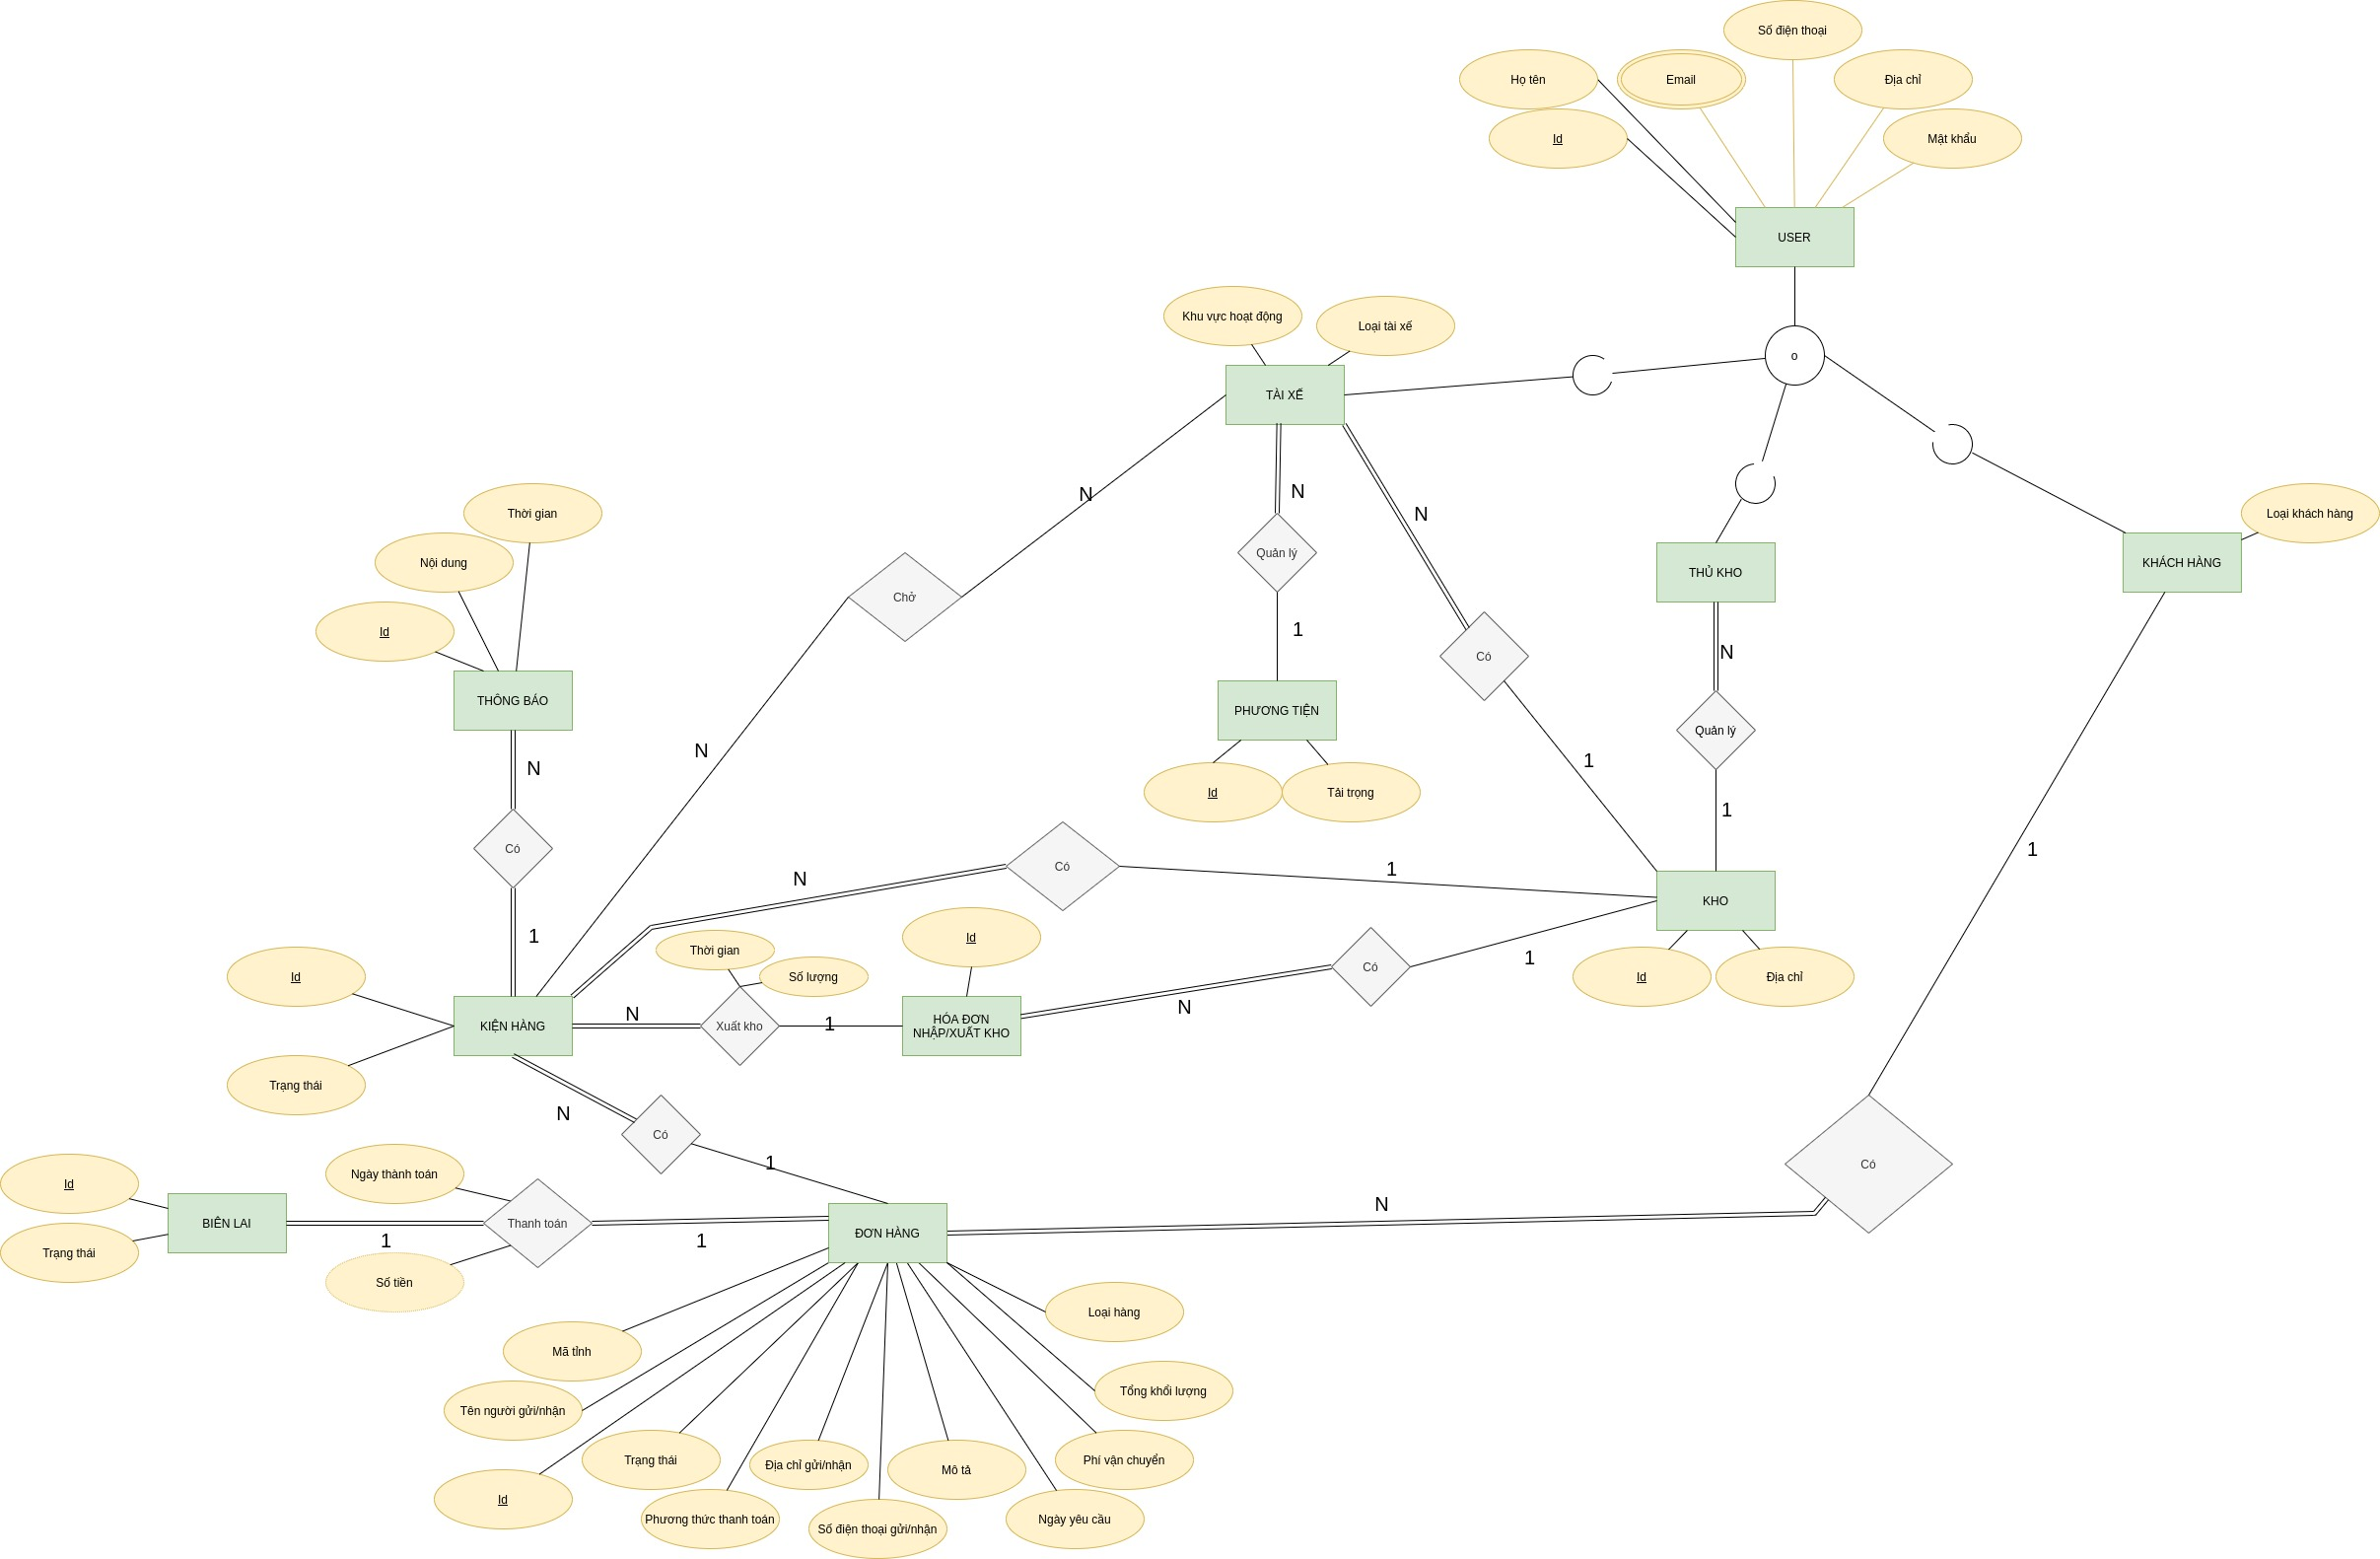
\includegraphics[angle=90, width=15cm, height=20cm]{Images/ERD.jpg}
			\centering
			\linebreak
			\caption{Lược đồ ERD}
		\end{figure}
	
	\newpage
	
	\newpage
	
	Sau khi thiết kế ERD nhóm tiến hành chuyển đổi thành các bảng tương ứng trong database như sau:
	
	\begin{itemize}
		\item \textbf{Order}
		
		\begin{table}[H]
			\centering\begin{tabular}{|l|m{30em}|}
				\hline 
				orderId & Mã đơn hàng\\
				\hline 
				assignedDrivers & Lưu danh sách tài xế đang được gán để đi lấy hàng \\ 
				\hline
				countcompletesuborder & Đếm số lượng kiện hàng đã hoàn tất \\
				\hline 
				driverIds & Danh sách các tài xế vận chuyển đơn hàng \\
				\hline
				fee & Phí vận chuyển \\
				\hline
				isDirectlyReceive & Người nhận có nhận trực tiếp hay không \\
				\hline
				isDirectlySend & Người gửi có gửi trực tiếp hay không \\
				\hline
				destStockId & Mã kho đích \\
				\hline
				detailOrder & Chi tiết đơn hàng \\
				\hline
				description & Mô tả đơn hàng \\
				\hline
				orderStatus & Trạng thái đơn hàng \\
				\hline
				orderTime & Thời gian tạo đơn hàng \\
				\hline
				paymentSide & Người thanh toán \\
				\hline
				paymentStatus & Trạng thái thanh toán \\
				\hline
				provinceCode & Mã tỉnh thành \\
				\hline
				remainWeight & Khối lượng còn lại \\
				\hline
				srcStockId & Mã kho nguồn \\
				\hline
				subOrderIds & Danh sách các kiện hàng tạo thành \\
				\hline
				totalWeight & Tổng khối lượng đơn hàng \\
				\hline
				userId & Mã khách hàng \\
				\hline
				value & Giá trị đơn hàng \\
				\hline
			\end{tabular}
			\caption{Schema Order}
		\end{table}
	
	\newpage
	
		\item \textbf{SubOrder}
		
		\begin{table}[H]
			\centering\begin{tabular}{|l|m{30em}|}
				\hline 
				subOrderId & Mã kiện hàng\\
				\hline 
				destDriverId & Mã tài xế đi giao \\ 
				\hline
				destDriverName & Tên tài xế đi giao \\
				\hline 
				destDriverPhone & Số điện thoại tài xế đi giao \\
				\hline
				destStockId & Mã kho đích \\
				\hline
				driverId & Mã tài xế đi lấy \\
				\hline
				driverName & Tên tài xế đi lấy \\
				\hline
				driverPhone & Số điện thoại tài xế đi lấy \\
				\hline
				externalDriverId & Mã tài xế liên tỉnh \\
				\hline
				externalDriverName & Tên tài xế liên tỉnh \\
				\hline
				externalDriverPhone & Số điện thoại tài xế liên tỉnh \\
				\hline
				issue & Nội dung vấn đề phát sinh \\
				\hline
				orderId & Mã đơn hàng \\
				\hline
				subOrderStatus & Trạng thái kiện hàng \\
				\hline
				provinceCode & Mã tỉnh thành \\
				\hline
				srcStockId & Mã kho nguồn \\
				\hline
				subOrderTime & Thời gian tạo kiện hàng \\
				\hline
				timeHistory & Danh sách thời gian update trạng thái đơn hàng \\
				\hline
				userId & Mã người dùng \\
				\hline
				weight & Khối lượng kiện hàng \\
				\hline
			\end{tabular}
			\caption{Schema SubOrder}
		\end{table}
	
	
	
		\item \textbf{ImportInfo}
		
		\begin{table}[H]
			\centering\begin{tabular}{|l|m{30em}|}
				\hline 
				id & Mã nhập kho\\
				\hline 
				driverId & Mã tài xế nhập kho\\ 
				\hline
				driverName & Tên tài xế nhập kho \\
				\hline 
				driverPhone & Số điện thoại tài xế nhập kho \\
				\hline
				importTime & Thời gian nhập kho \\
				\hline
				stockId & Mã kho \\
				\hline
				stockkeeperId & Mã thủ kho \\
				\hline
				stockkeeperName & Tên thủ kho \\
				\hline
				stockkeeperPhone & Số điện thoại thủ kho \\
				\hline
				subOrderIds & Danh sách kiện hàng nhập kho \\
				\hline
			\end{tabular}
			\caption{Schema ImportInfo}
		\end{table}
	
	\newpage
	
	
		\item \textbf{ExportInfo}
		
		\begin{table}[H]
			\centering\begin{tabular}{|l|m{30em}|}
				\hline 
				id & Mã xuất kho\\
				\hline 
				driverId & Mã tài xế xuất kho\\ 
				\hline
				driverName & Tên tài xế xuất kho \\
				\hline 
				driverPhone & Số điện thoại tài xế xuất kho \\
				\hline
				importTime & Thời gian xuất kho \\
				\hline
				stockId & Mã kho \\
				\hline
				stockkeeperId & Mã thủ kho \\
				\hline
				stockkeeperName & Tên thủ kho \\
				\hline
				stockkeeperPhone & Số điện thoại thủ kho \\
				\hline
				subOrderIds & Danh sách kiện hàng xuất kho \\
				\hline
			\end{tabular}
			\caption{Schema ExportInfo}
		\end{table}

	
		\item \textbf{SupportRequest}
		
		\begin{table}[H]
			\centering\begin{tabular}{|l|m{30em}|}
				\hline 
				id & Mã yêu cầu\\
				\hline 
				userId & Mã khách hàng\\
				\hline 
				orderId & Mã đơn hàng\\ 
				\hline
				reqTime & Thời gian yêu cầu \\
				\hline 
				content & Nội dung yêu cầu \\
				\hline
				emailAddress & Địa chỉ mail của khách hàng \\
				\hline
				reply & Thông tin phản hồi \\
				\hline
			\end{tabular}
			\caption{Schema SupportRequest}
		\end{table}
	
		\item \textbf{StatisticFee}
		
		\begin{table}[H]
			\centering\begin{tabular}{|l|m{30em}|}
				\hline 
				date & Ngày tháng năm theo format yyMMđd\\
				\hline 
				totalFee & Mã khách hàng\\
				\hline 
			\end{tabular}
			\caption{Schema StatisticFee}
		\end{table}
	
	
		\item \textbf{StatisticTrans}
		
		\begin{table}[H]
			\centering\begin{tabular}{|l|m{30em}|}
				\hline 
				date & Ngày tháng năm theo format yyMMđd\\
				\hline 
				transSuccess & Số đơn hàng thành công\\
				\hline 
				transCancel & Số đơn hàng bị hủy\\
				\hline 
				transFail & Số đơn hàng thất bại\\
				\hline 
			\end{tabular}
			\caption{Schema StatisticFee}
		\end{table}
	
	\newpage
	
		\item \textbf{Driver}
		
		\begin{table}[H]
			\centering\begin{tabular}{|l|m{30em}|}
				\hline 
				id & Mã tài xế\\
				\hline 
				area & Mã khu vực hoạt động của tài xế\\
				\hline 
				status & Trạng thái hoạt động của tài xế\\
				\hline 
				vehicleId & Mã phương tiện\\
				\hline 
			\end{tabular}
			\caption{Schema Driver}
		\end{table}
	
		\item \textbf{Role}
		
		\begin{table}[H]
			\centering\begin{tabular}{|l|m{30em}|}
				\hline 
				userId & Mã user\\
				\hline 
				role & Vai trò của user\\
				\hline 
			\end{tabular}
			\caption{Schema Role}
		\end{table}
	
		\item \textbf{Stocker}
		
		\begin{table}[H]
			\centering\begin{tabular}{|l|m{30em}|}
				\hline 
				id & Mã thủ kho\\
				\hline 
				areaId & Mã kho\\
				\hline 
			\end{tabular}
			\caption{Schema Stocker}
		\end{table}
	
		\item \textbf{User}
		
		\begin{table}[H]
			\centering\begin{tabular}{|l|m{30em}|}
				\hline 
				id & Mã user\\
				\hline 
				address & Địa chỉ\\
				\hline 
				email & Email\\
				\hline 
				password & Mật khẩu\\
				\hline 
				phone & Số điện thoại\\
				\hline 
				provinceCode & Mã tỉnh\\
				\hline 
				username & Tên tài khoản\\
				\hline 
			\end{tabular}
			\caption{Schema User}
		\end{table}
	
		\item \textbf{Vehicle}
		
		\begin{table}[H]
			\centering\begin{tabular}{|l|m{30em}|}
				\hline 
				id & Mã phương tiện\\
				\hline 
				currentWeight & Trọng tải hiện tại\\
				\hline 
				totalWeight & Trọng tải\\
				\hline 
				number & Biển số\\
				\hline 
			\end{tabular}
			\caption{Schema Vehicle}
		\end{table}
	
	\newpage
	
		\item \textbf{Warehouse}
		
		\begin{table}[H]
			\centering\begin{tabular}{|l|m{30em}|}
				\hline 
				id & Mã kho\\
				\hline 
				address & Địa chỉ kho\\
				\hline 
				areaCode & Mã khu vực\\
				\hline 
			\end{tabular}
			\caption{Schema Warehouse}
		\end{table}


	\end{itemize}



	



	
    \chapter{Hiện thực hệ thống}

\section{Công nghệ sử dụng}

	Để xây dựng một hệ thống lớn, phức tạp, khả năng chịu tải cao và dễ mở rộng như vậy thì nhóm đã sử dụng rất nhiều thư viện cả phía FrontEnd lẫn BackEnd. Sau đây là một số công nghệ nổi bật.
	
	\begin{table}[!htp]
		\centering\begin{tabular}{|l|l|m{20em}|}
			\hline 
			Thư viện, framework & Phiên bản & Chức năng\\
			\hline 
			SpringBoot & 2.2.6 & Giúp tạo service nhanh chóng và dễ dàng  \\
			\hline 
			guava & 20.0 & Cung cấp các hàm để xử lý Collections \\
			\hline 
			data-jpa & 2.2.6 & Cung cấp các API để làm việc với database \\
			\hline 
			redisson & 3.12.3 & Cung cấp API để service tương tác với Redis server\\
			\hline 
			mysql-connector-java & 2.2.6 & Giúp kết nối service đến database Mysql \\
			\hline 
			gson & 2.8.2 & Cung cấp các hàm để làm việc với JSON object \\
			\hline 
			spring-kafka &  2.2.6 & Cung cấp API để tương tác với Kafka brokers \\
			\hline 
			httpclient & 4.5.12 & Hỗ trợ việc gửi HTTP Request để giao tiếp với service khác \\
			\hline 
			log4j2 &  2.2.6 & Hỗ trợ cơ chế ghi log \\
			\hline 
			data-cassandra & 2.2.6 & Giúp kết nối service đến database Cassandra \\
			\hline 
			activemq & 2.2.6  & Cung cấp API để tương tác với ActiveMQ server \\
			\hline 
			spring-boot-starter-mail & 2.2.6 & Giúp hiện thực chức năng gửi mail \\
			\hline
		\end{tabular}
		\caption{Công nghệ sử dụng}
	\end{table}


\section{Quản lý mã nguồn}
	
	Để các thành viên trong nhóm có thể cùng nhau phát triển mà không gặp xung đột gì thì cả nhóm sử dụng Git để quản lý mã nguồn. 
	
	Git là hệ thống kiểm soát phiên bản phân tán mà nguồn mở. Các dự án thực tế thường có nhiều nhà phát triển làm việc song song. Vì vậy, một hệ thống kiểm soát phiên bản như Git là cần thiết để đảm bảo không có xung đột mã giữa các nhà phát triển. Ngoài ra, các yêu cầu trong dự án thay đổi thường xuyên. Vì vậy, cần một hệ thống cho phép nhà phát triển quay lại phiên bản cũ hơn của mã nguồn.
	
	\begin{figure}[!ht]
		
\includegraphics[width=0.8\textwidth]{Images/gitlab.png}
		\centering
		\linebreak
		\caption{Giới thiệu về Gitlab}
	\end{figure}
	
	Về việc lưu trữ mã nguồn thì nhóm sử dụng Gitlab. GitLab khá nổi tiếng và là một mã nguồn mở của máy chủ Git được thực hiện bởi hơn 50.000 tổ chức. Trong vài năm gần đây Gitlad đã phát triển mạnh mẽ với sự hỗ trợ của cộng đồng mạng, hàng nghìn người sử dụng trên một máy chủ duy nhất hoặc một số máy chủ hoạt động tương tự.
	

\section{Phương pháp deploy service}



\section{Kết quả hiện thực}

Sau quá trình dài thực hiện luận văn, sử dụng những công nghệ và kiên thức được đưa
ra trong các phần trước, nhóm đã hoàn thành một hệ thống vận chuyển hàng hóa liên tỉnh tương đối hoàn chỉnh.

\subsection{Chức năng đăng nhập, đăng kí}

	\begin{itemize}
		\item \textbf{Đăng kí}
			\begin{figure}[H]
				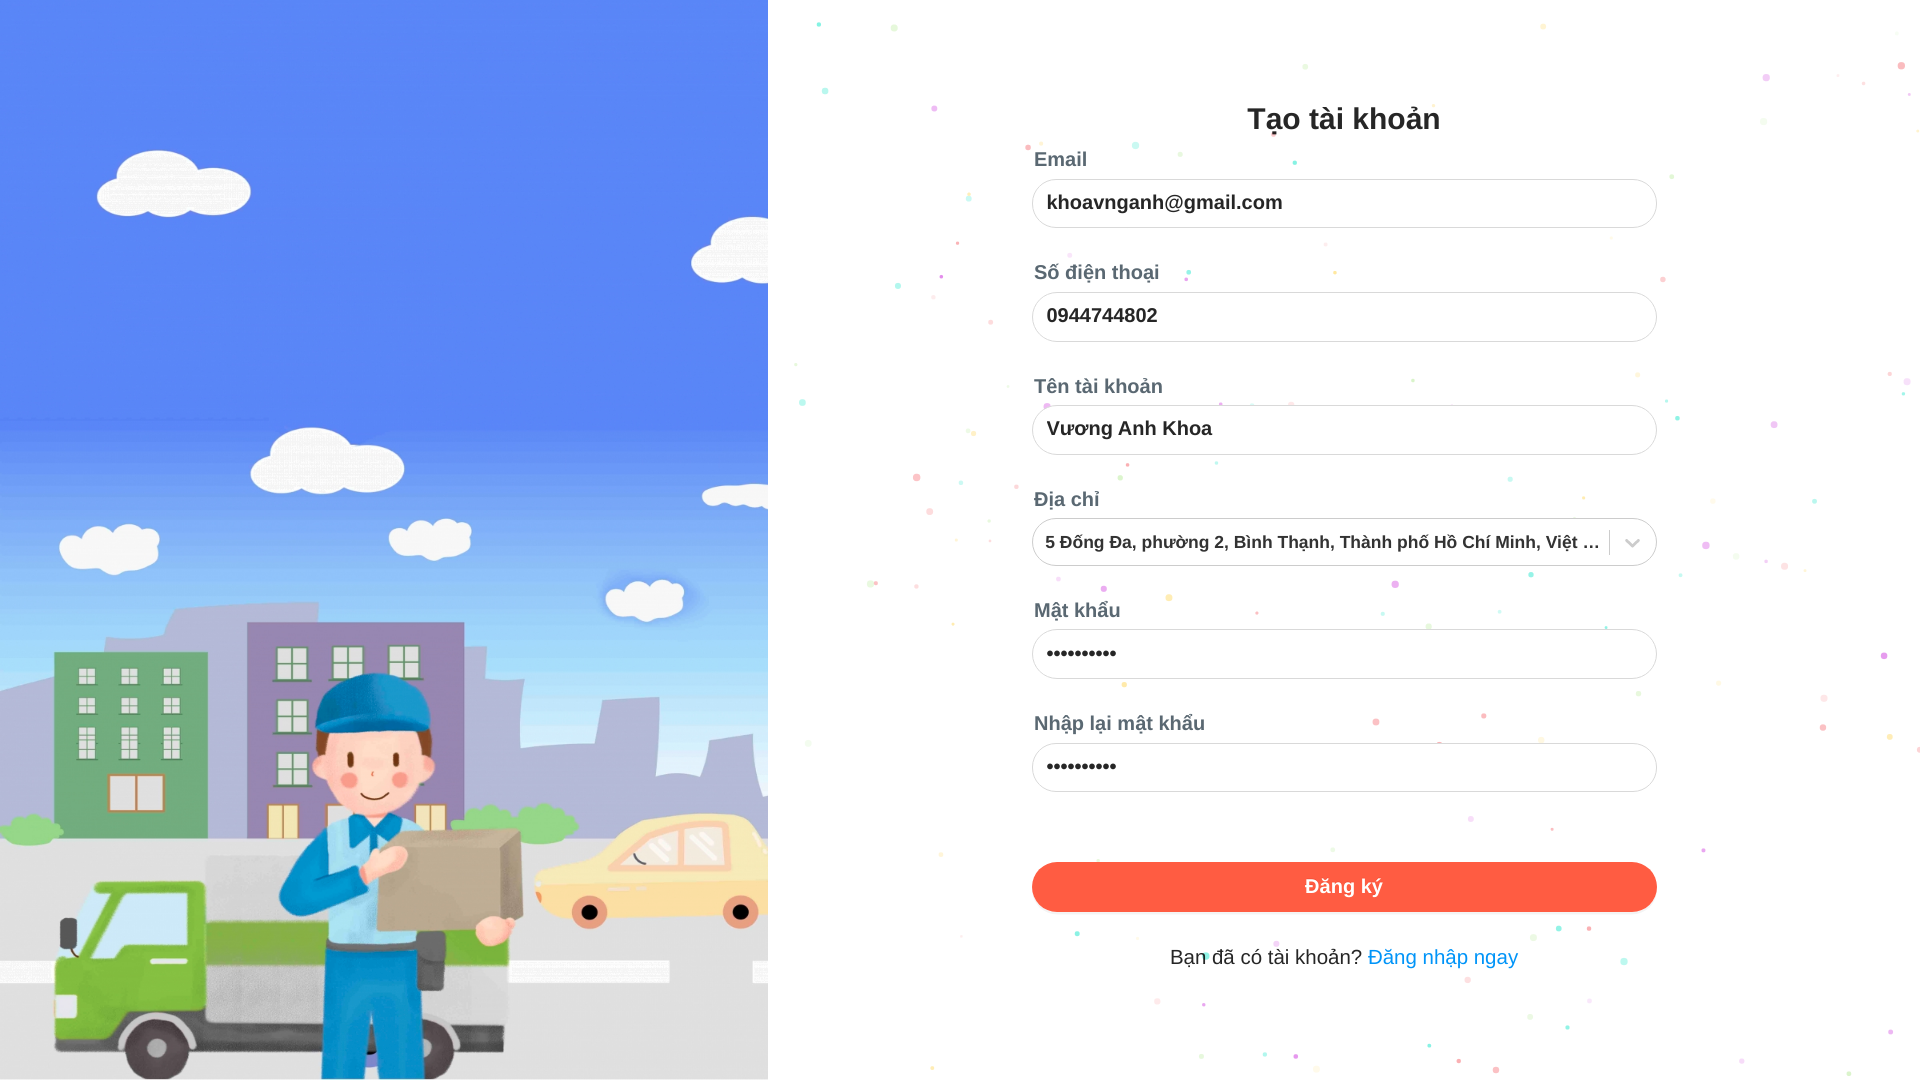
\includegraphics[width=1\textwidth]{/Auth/SignUp.png}
				\centering
				\caption{Giao diện đăng kí dành cho người muốn gửi đơn hàng}
			\end{figure}
		
		\item \textbf{Đăng nhập}
		\begin{figure}[H]
			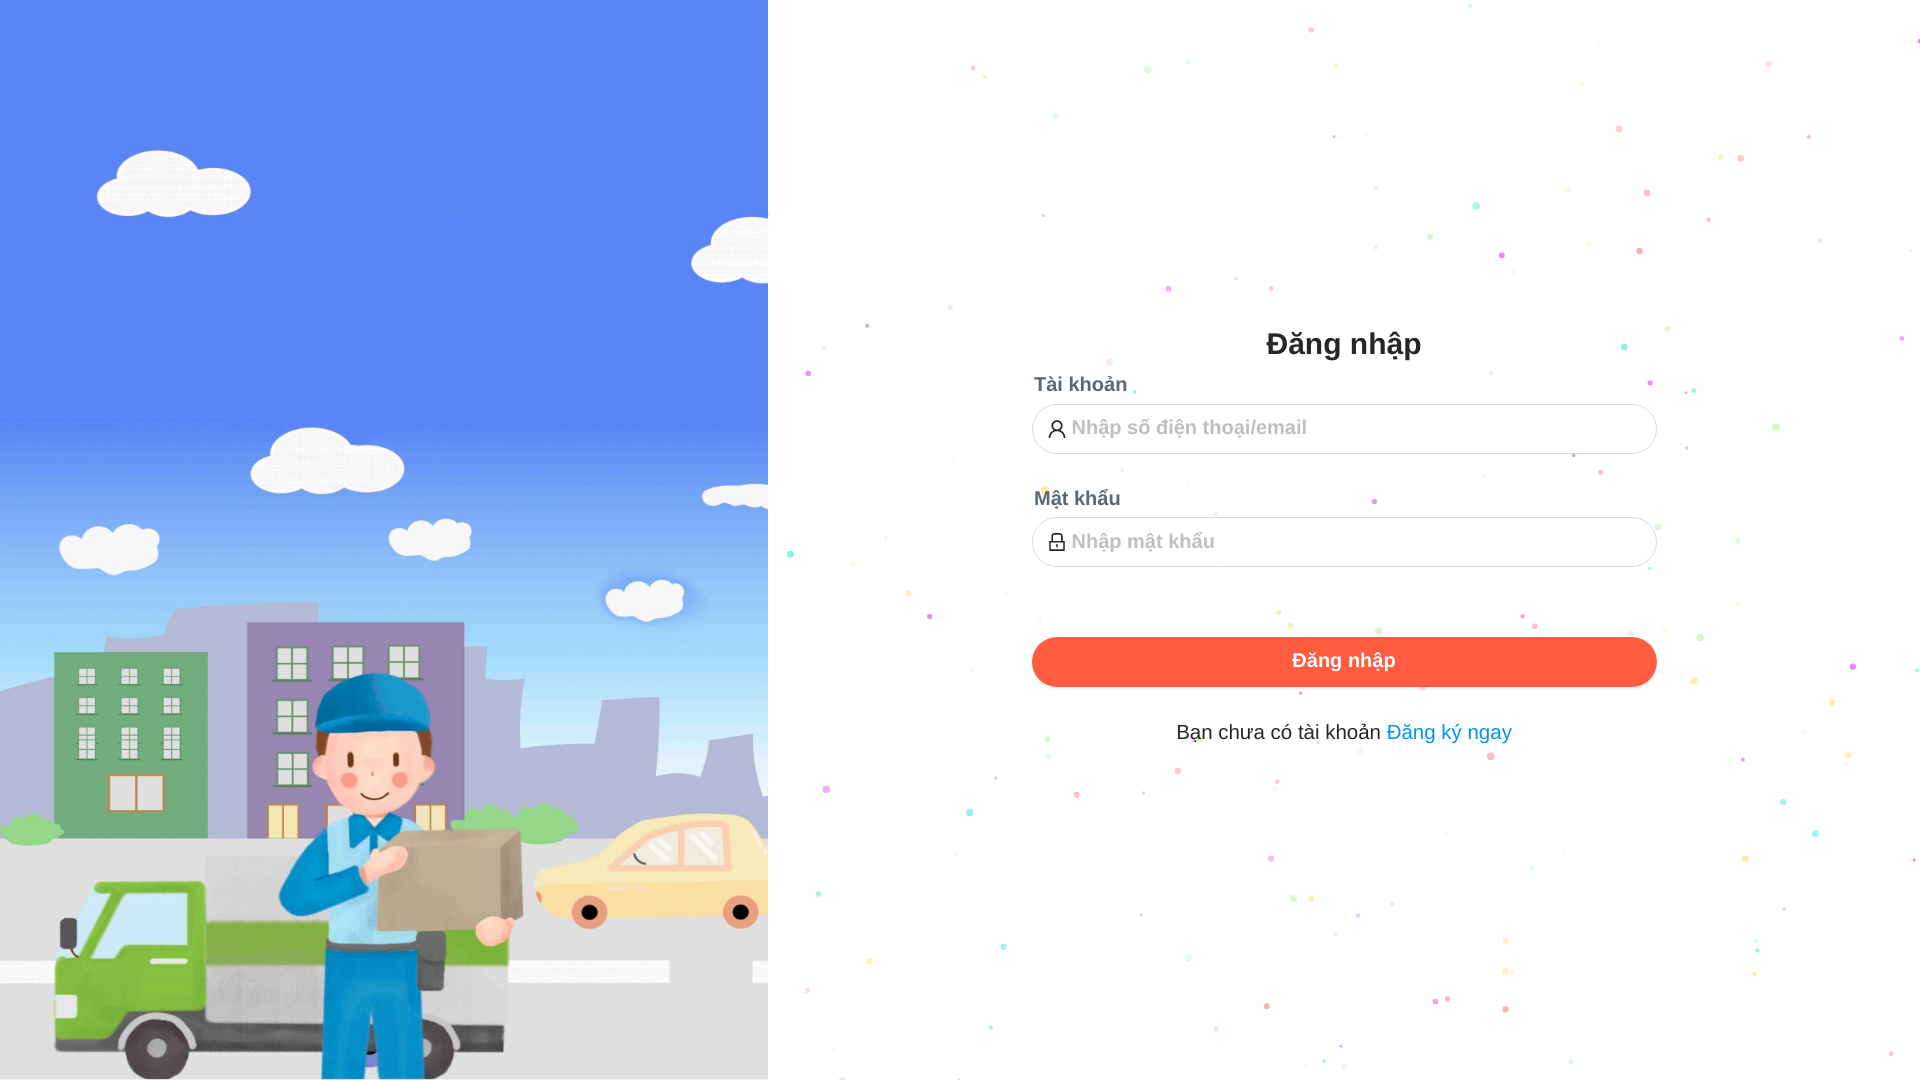
\includegraphics[width=1\textwidth]{/Auth/SignIn.png}
			\centering
			\caption{Giao diện đăng nhập dành cho actor của hệ thống}
		\end{figure}
	\end{itemize}

\subsection{Chức năng dành cho người gửi}
	\begin{itemize}
		\item \textbf{Lên đơn hàng}
		\begin{figure}[H]
			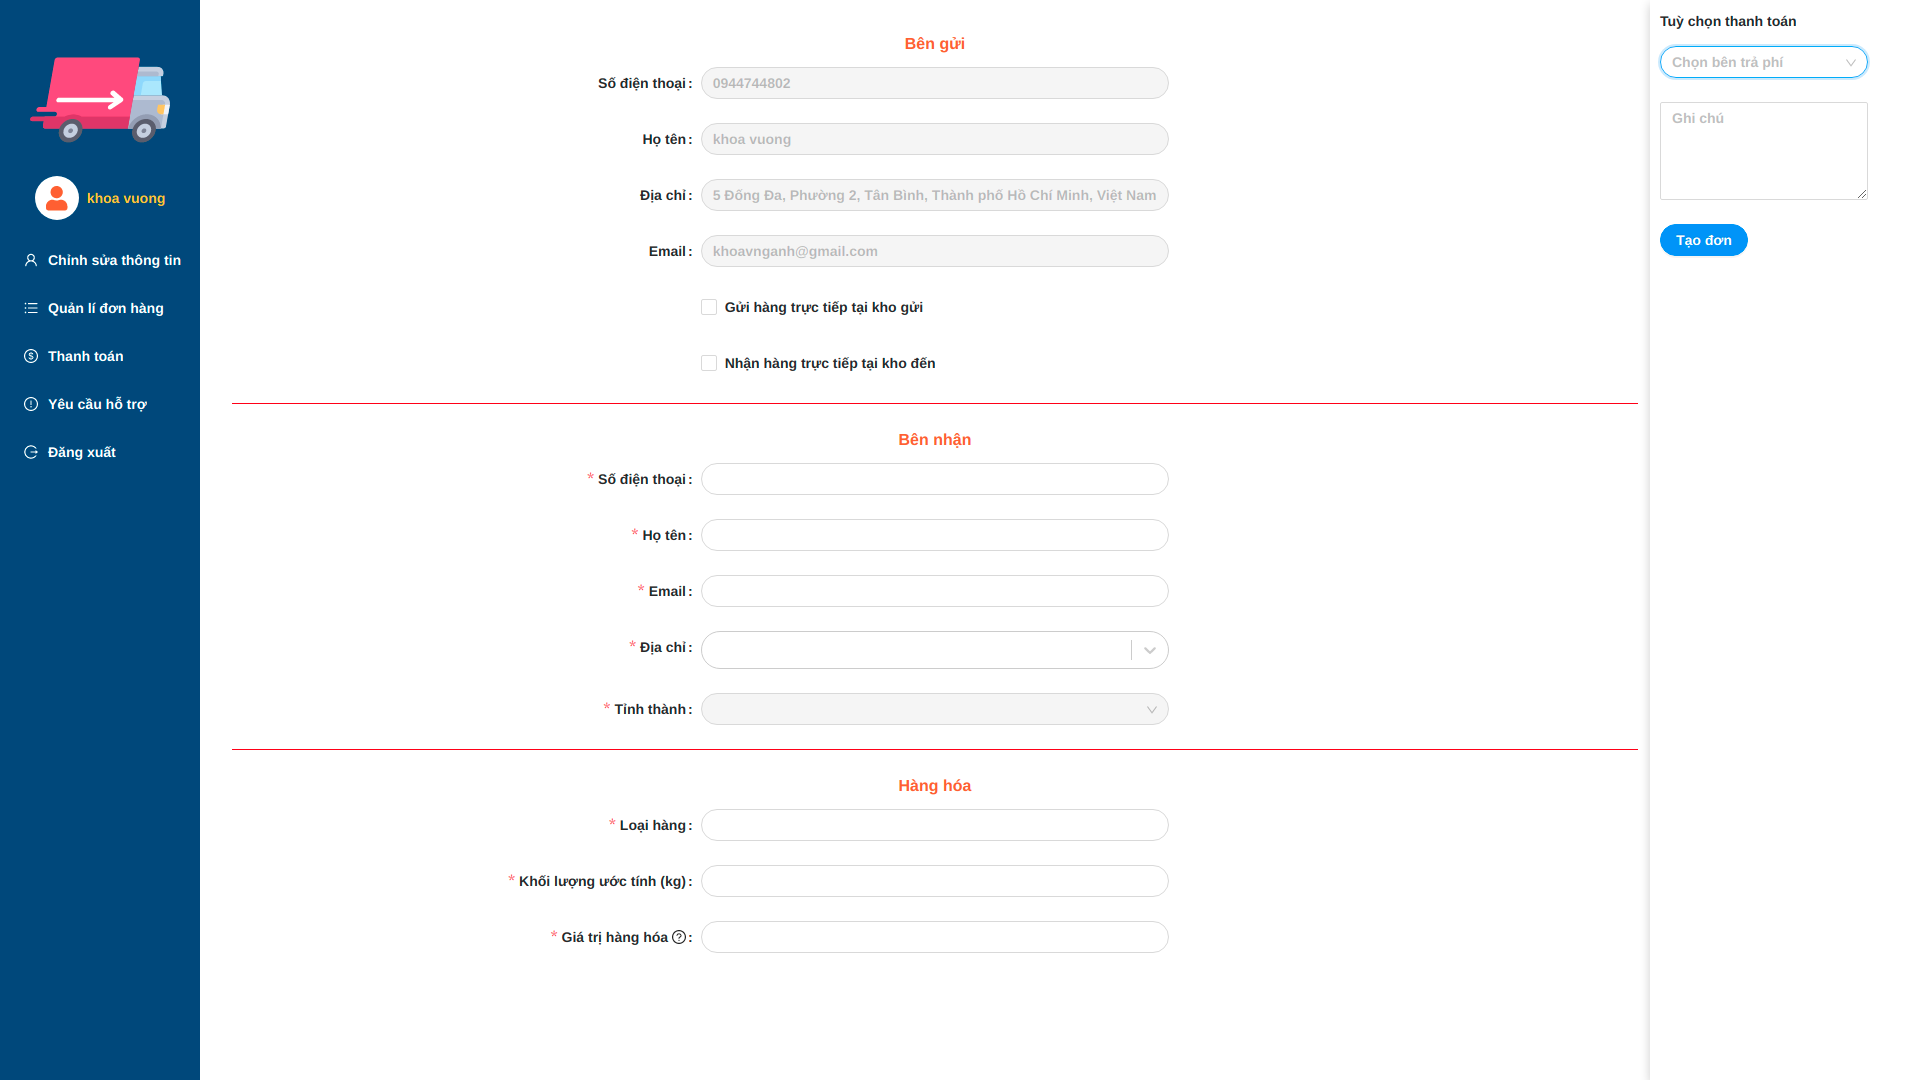
\includegraphics[width=1\textwidth]{/sender/create_order.png}
			\centering
			\caption{Giao diện điền thông tin để lên đơn hàng}
		\end{figure}
	
		\begin{figure}[H]
			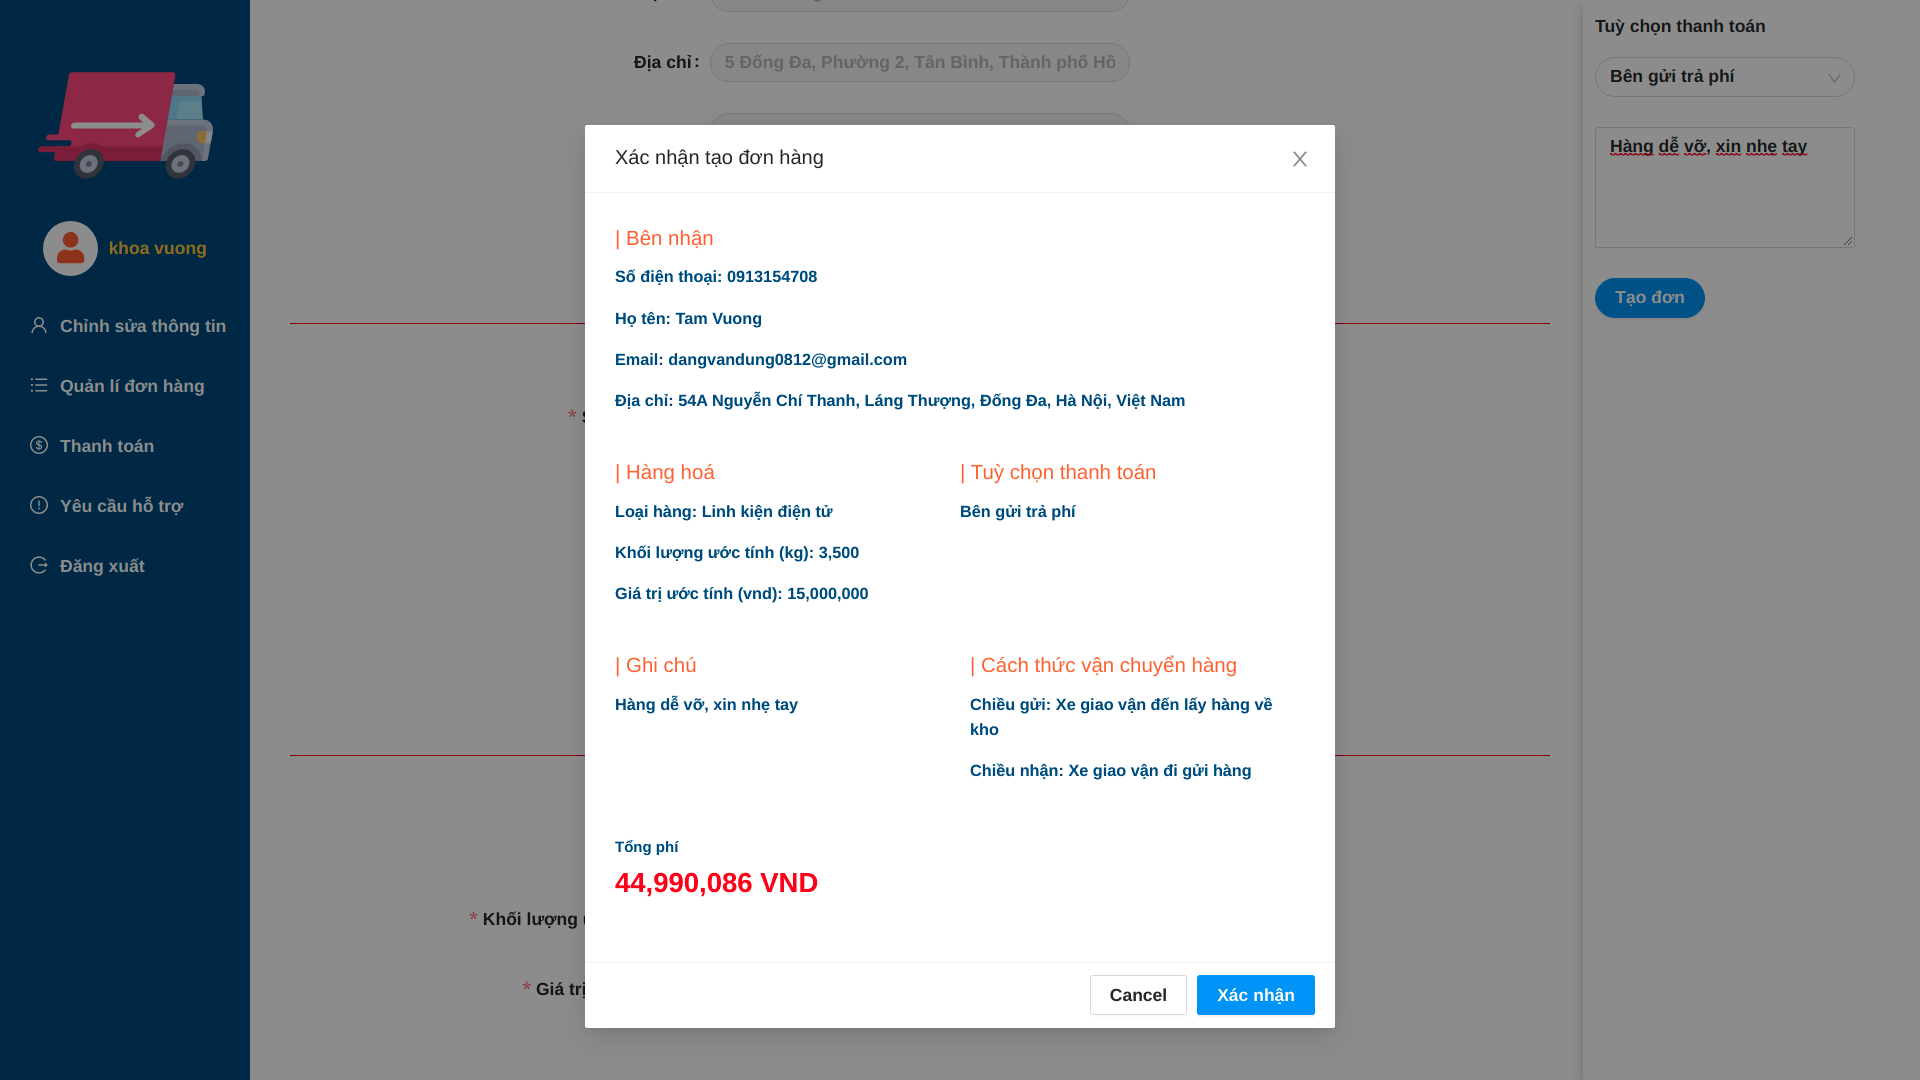
\includegraphics[width=1\textwidth]{/sender/create_order_model.png}
			\centering
			\caption{Thông tin xác nhận đơn hàng muốn tạo}
		\end{figure}
		Khung nhập địa chỉ hỗ trợ gợi ý địa chỉ nhờ sử dụng Google Place Autocomplete API. Khi ấn nút tạo đơn sẽ có màn hình chờ để phía server trả về phí vận chuyển.
		
		\item \textbf{Xem danh sách đơn hàng}
		\begin{figure}[H]
			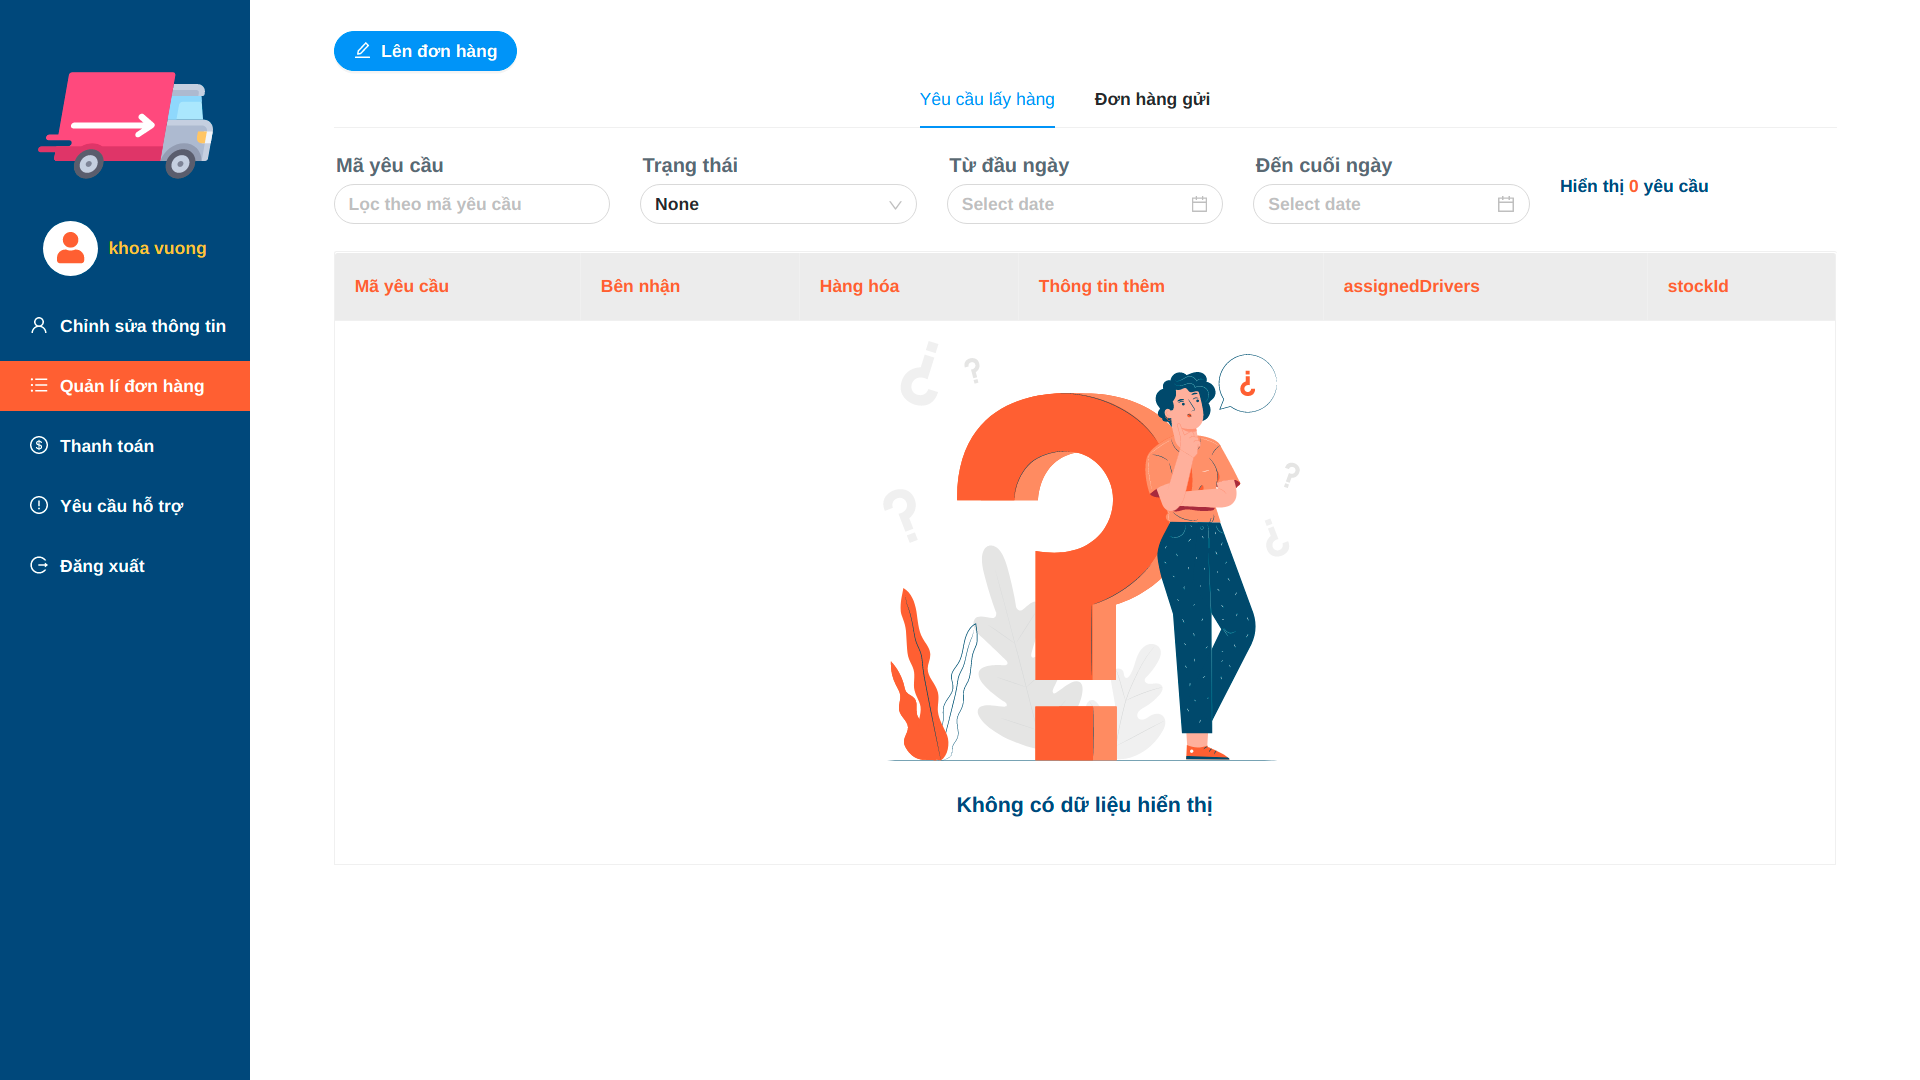
\includegraphics[width=1\textwidth]{/sender/request_empty.png}
			\centering
			\caption{Giao diện list yêu cầu của người gửi (Rỗng)}
		\end{figure}
		
		\begin{figure}[H]
			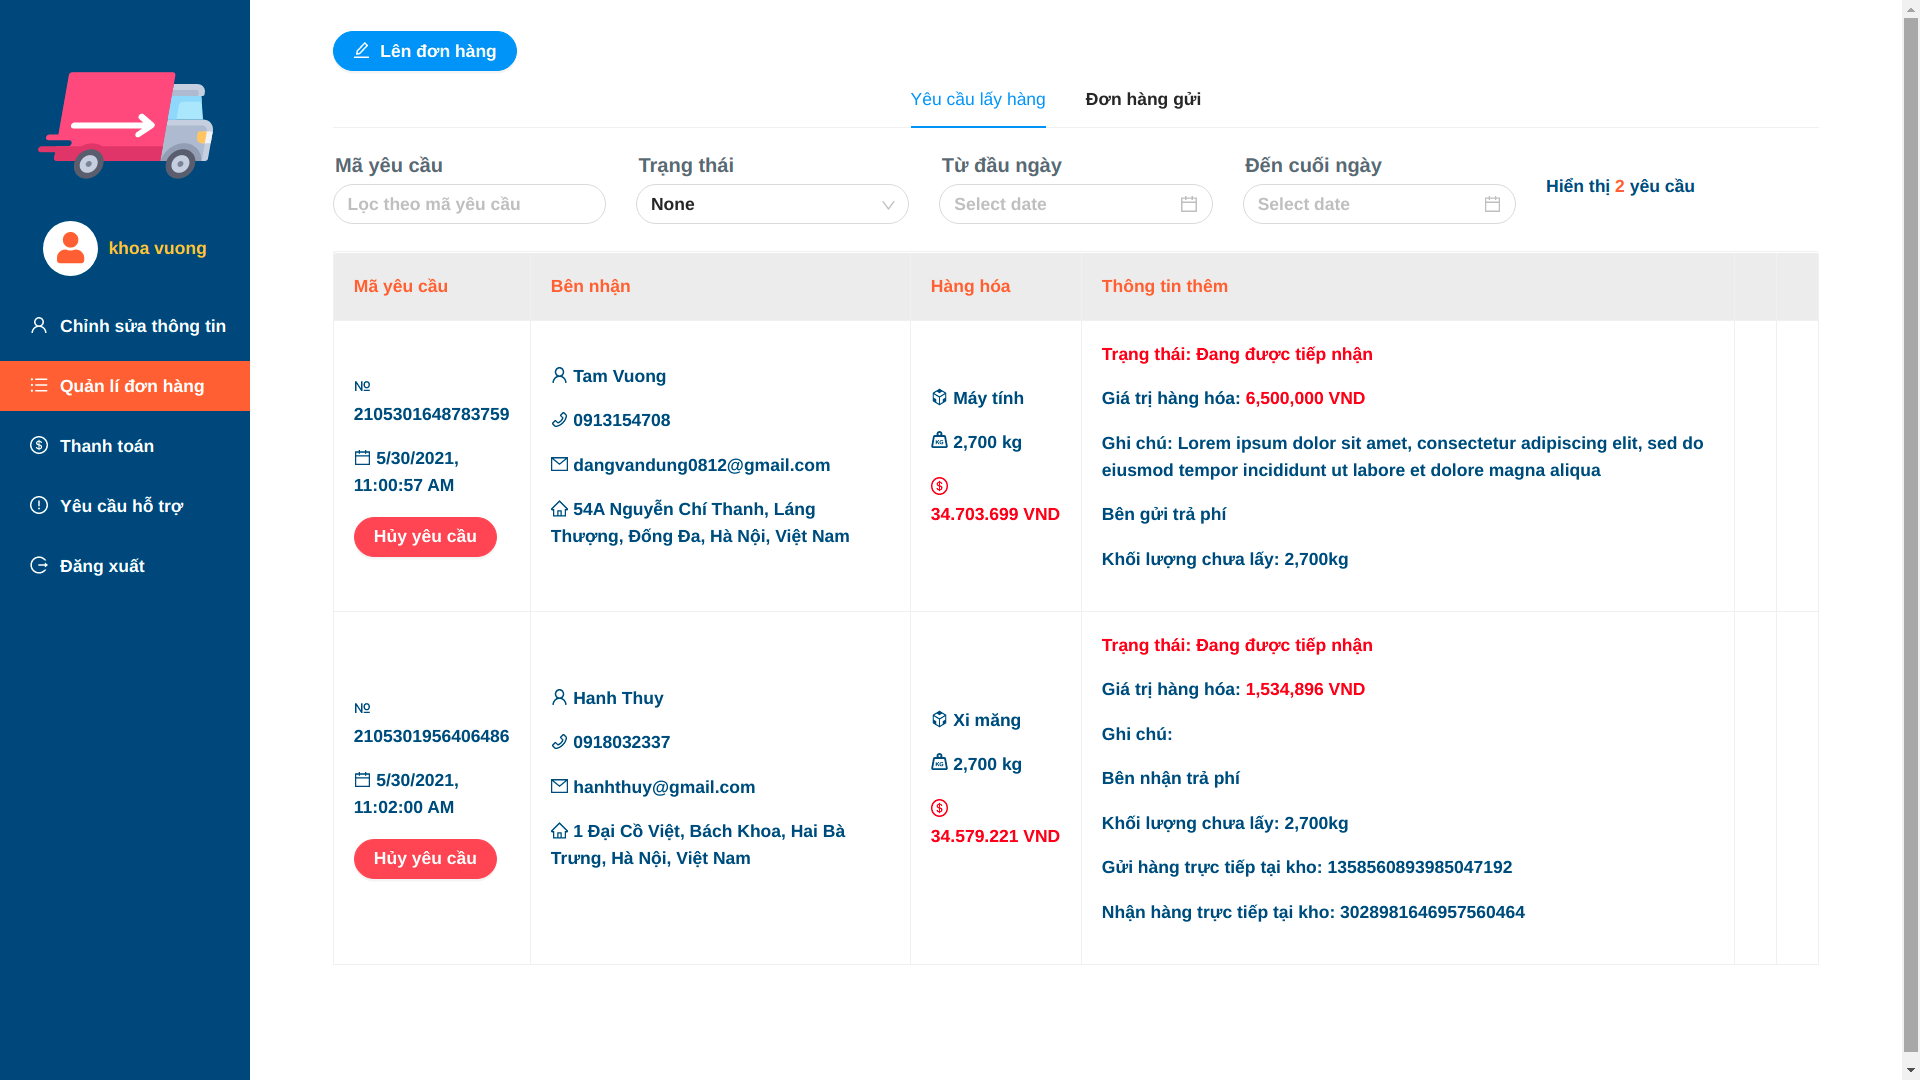
\includegraphics[width=1\textwidth]{/sender/request_list.png}
			\centering
			\caption{Giao diện list yêu cầu của người gửi (Có yêu cầu)}
		\end{figure}
		Các yêu cầu đã tạo có thể được lọc theo những tiêu chí: Mã yêu cầu, trạng thái (Gồm 4 trạng thái yêu cầu đã nêu trong phần trước), thời gian tạo đơn hàng.
		
		\item \textbf{Xem danh sách các kiện hàng}
		\begin{figure}[H]
			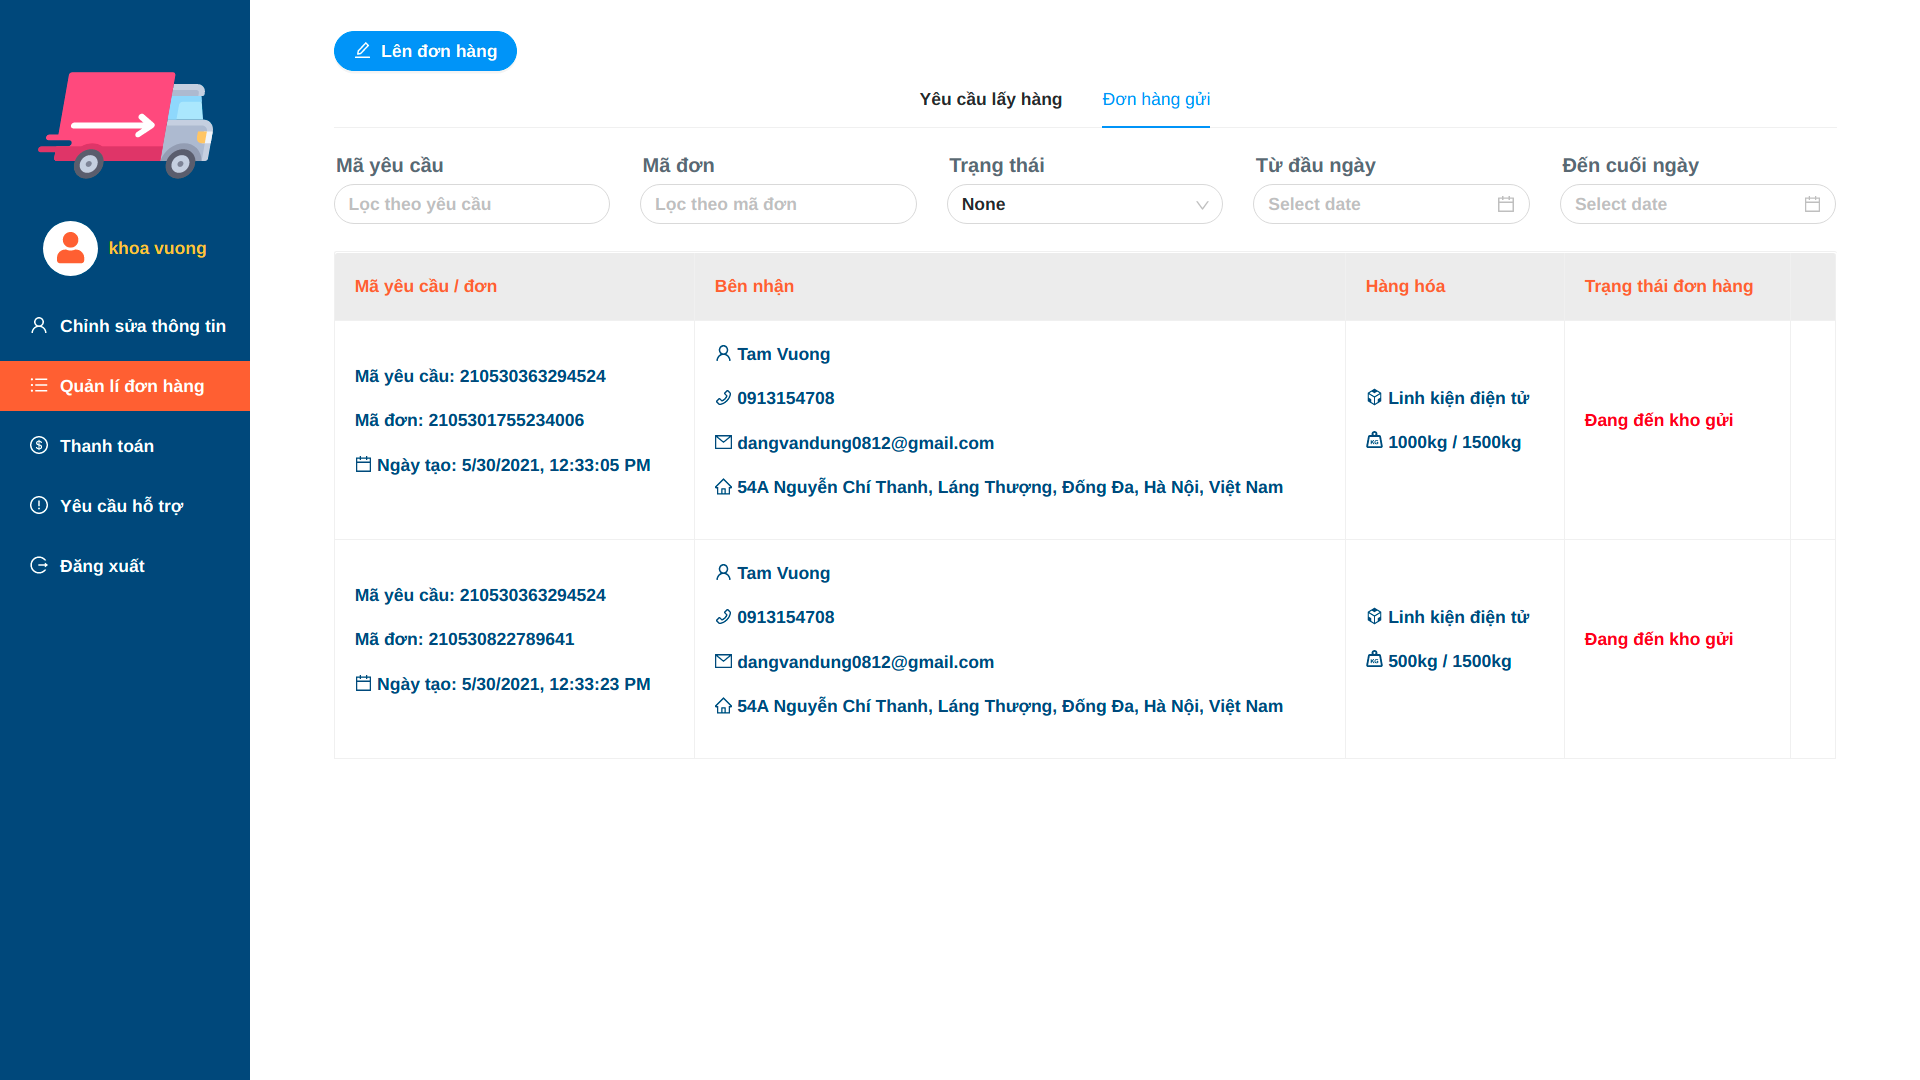
\includegraphics[width=1\textwidth]{/sender/sender_suborders.png}
			\centering
			\caption{Giao diện xem danh sách các đơn hàng nhỏ được tách từ yêu cầu}
		\end{figure}
	
		\item \textbf{Chỉnh sửa thông tin của người gửi}
		
		\begin{figure}[H]
			\includegraphics[width=1\textwidth]{/sender/sender_info.png}
			\centering
			\caption{Giao diện chỉnh sửa thông tin của người gửi}
		\end{figure}
		
		
	\end{itemize}


\subsection{Chức năng dành cho tài xế}
\begin{itemize}
	\item \textbf{Tìm những yêu cầu được gán}
	\begin{figure}[H]
		\includegraphics[width=1\textwidth]{/driver/driver_find_order.png}
		\centering
		\caption{Giao diện tìm những yêu cầu được gán}
	\end{figure}
	
	\begin{figure}[H]
		\includegraphics[width=1\textwidth]{/driver/driver_find_modal.png}
		\centering
		\caption{Giao diện xác nhận lại thông tin yêu cầu muốn nhận}
	\end{figure}
	
	
	\item \textbf{Xem danh sách đơn hàng}
	\begin{figure}[H]
		\includegraphics[width=1\textwidth]{/driver/driver_current_order.png}
		\centering
		\caption{Giao diện xem thông tin đơn hàng đang đến lấy}
	\end{figure}
	
	\begin{figure}[H]
		\includegraphics[width=1\textwidth]{/driver/driver_current_modal.png}
		\centering
		\caption{Giao diện xác nhận lại thông tin đơn hàng đang muốn nhận}
	\end{figure}


	
	\item \textbf{Xem danh sách các kiện hàng}
	\begin{figure}[H]
		\includegraphics[width=1\textwidth]{/driver/driver_intruck.png}
		\centering
		\caption{Giao diện xem thông tin các đơn hàng đang ở trong xe}
	\end{figure}
	
	\item \textbf{Báo cáo vấn đề}
	
	\begin{figure}[H]
		\includegraphics[width=1\textwidth]{/driver/driver_issue.png}
		\centering
		\caption{Giao diện báo cáo vấn đề ghi gặp sự cố}
	\end{figure}


	\item \textbf{Xem lịch sử giao nhận hàng}
	
	\begin{figure}[H]
		\includegraphics[width=1\textwidth]{/driver/driver_history.png}
		\centering
		\caption{Giao diện xem lịch sử giao nhận hàng}
	\end{figure}
	
\end{itemize}





\subsection{Chức năng dành cho thủ kho}
\begin{itemize}
	\item \textbf{Nhập hàng}
	\begin{figure}[H]
		\includegraphics[width=1\textwidth]{/stockkeeper/stock_import_driver.png}
		\centering
		\caption{Giao diện nhập ID của tài xế để nhập các đơn hàng trong xe tài xế vào kho}
	\end{figure}

	\begin{figure}[H]
		\includegraphics[width=1\textwidth]{/stockkeeper/stock_import_customer.png}
		\centering
		\caption{Nhập ID của khách hàng để nhập đơn vào kho}
	\end{figure}

	\begin{figure}[H]
		\includegraphics[width=1\textwidth]{/stockkeeper/stock_import_customer_detail.png}
		\centering
		\caption{Cho phép nhập khối lượng mà khách muốn nhập vào kho}
	\end{figure}
	
	\begin{figure}[H]
		\includegraphics[width=1\textwidth]{/stockkeeper/stock_import_driver_prompt.png}
		\centering
		\caption{Xác nhận nhập hàng vào kho}
	\end{figure}
	
	\begin{figure}[H]
		\includegraphics[width=1\textwidth]{/stockkeeper/stock_import_driver_pdf.png}
		\centering
		\caption{Nhập hàng thành công và cho thủ kho có thể tài phiếu nhập kho}
	\end{figure}

	\begin{figure}[H]
		\includegraphics[width=1\textwidth]{/stockkeeper/stock_history_detail.png}
		\centering
		\caption{Thông tin chi tiết của một lần nhập/xuất đơn hàng (Cho phép tải pdf về)}
	\end{figure}
	
	\begin{figure}[H]
		\includegraphics[width=1\textwidth]{/stockkeeper/stock_pdf.png}
		\centering
		\caption{Format mẫu của 1 đơn nhập/xuất kho}
	\end{figure}
	
	
	\item \textbf{Xem danh sách đơn hàng}
	\begin{figure}[H]
		\includegraphics[width=1\textwidth]{/stockkeeper/stock_list.png}
		\centering
		\caption{Danh sách các đơn hàng trong kho}
	\end{figure}

	\begin{figure}[H]
		\includegraphics[width=1\textwidth]{/stockkeeper/stock_history.png}
		\centering
		\caption{Lịch sử nhập/xuất kho}
	\end{figure}
	
	Chức năng xuất kho có giao diện và tính năng tương tự lúc nhập kho.
	
\end{itemize}




\subsection{Chức năng dành cho Quản lý}
\begin{itemize}
	\item \textbf{Quản lý tài xế}
	\begin{figure}[H]
		\includegraphics[width=1\textwidth]{/admin/admin_list_driver.png}
		\centering
		\caption{Xem danh sách các tài xế trong hệ thống}
	\end{figure}
	
	
	\item \textbf{Quản lý thủ kho}
	\begin{figure}[H]
		\includegraphics[width=1\textwidth]{/admin/admin_list_stock.png}
		\centering
		\caption{Xem danh sách các kho và thủ kho phụ trách của hệ thống}
	\end{figure}

	\item \textbf{Xem thống kê}
	\begin{figure}[H]
		\includegraphics[width=1\textwidth]{/admin/admin_statistic.png}
		\centering
		\caption{Xem thống kê đơn hàng và số tiền khách hàng đã thanh toán}
	\end{figure}

	\item \textbf{Thêm tài xế vào hệ thống}
	\begin{figure}[H]
		\includegraphics[width=1\textwidth]{/admin/admin_add_driver.png}
		\centering
		\caption{Thêm tài xế vào hệ thống}
	\end{figure}


	\item \textbf{Thêm thủ kho vào hệ thống}
	\begin{figure}[H]
		\includegraphics[width=1\textwidth]{/admin/admin_add_stock.png}
		\centering
		\caption{Thêm kho vào hệ thống}
	\end{figure}
	
	\begin{figure}[H]
		\includegraphics[width=1\textwidth]{/admin/admin_add_stock_keeper.png}
		\centering
		\caption{Thêm thủ kho vào hệ thống}
	\end{figure}

	\item \textbf{Xem yêu cầu hỗ trợ}
	\begin{figure}[H]
		\includegraphics[width=1\textwidth]{/admin/admin_requests_reply.png}
		\centering
		\caption{Giao diện trả lời những yêu cần cầu hỗ trợ từ khách hàng}
	\end{figure}
	
	\begin{figure}[H]
		\includegraphics[width=1\textwidth]{/admin/admin_requests_done.png}
		\centering
		\caption{Giao diện xem lại những yêu cầu hỗ trợ đã trả lời}
	\end{figure}

	\item \textbf{Xem báo cáo sự cố}
	\begin{figure}[H]
		\includegraphics[width=1\textwidth]{/admin/admin_issues.png}
		\centering
		\caption{Giao diện xem những sự cố báo cáo từ tài xế}
	\end{figure}


	\item \textbf{Xử lý sự cố}
	\begin{figure}[H]
		\includegraphics[width=1\textwidth]{/admin/admin_issues_reply.png}
		\centering
		\caption{Giao diện gán lại trạng thái cho những đơn có sự cố}
	\end{figure}
		
\end{itemize}
























    \chapter{Kiểm thử hệ thống}\label{chap:testing}
		Kiếm thử phần mềm là một việc rất quan trọng trong quy trình phát triển phần mềm.
        Để một hệ thống có thể đi vào hoạt động ổn định, các nhà phát triển cần kiểm tra tất
        cả tính năng, các thành phần của hệ thống, mọi thứ phải hoạt động một cách trơn tru
        mới có thể chuyển giao đến tay người sử dụng. Bất kỳ một lỗi nhỏ nào nếu không kiểm
        tra kỹ càng cũng có thể để lại hậu quả về sau, làm cho hệ thống không đáng tin cậy và
        không được sự hưởng ứng từ phía người dùng.\\
        
        Quy trình kiểm thử cần phải qua nhiều loại khác nhau: Unit test, Intergration test, System test, Acceptance test, Functional testing, Non Functional testing, End to end test... Hiện nay có rất nhiều thư viện kiểm thử hiệu quả và mạnh mẽ. Katalon Recorder là một extension dành cho chrome đã tích hợp tính năng kiểm thử vào trong nó để kiểm thử chức năng. Jmeter là công cụ để đo độ tải và performance của trang web và nhóm đã sử dụng K6 cloud platform có tích hợp jmeter để có thể kiểm thử phi chức năng cho trang web của nhóm.
		\section{Kiểm thử API}
		Đối với hệ thống nhóm xây dựng, các thành phần giao tiếp với nhau thông qua API. Vì vậy, cần phải kiểm thử riêng biệt các API trước khi tích hợp vào các bên. Nhóm chọn phần mềm Postman để kiểm thử các API.\\
		
		\newpage
		
		\textbf{API đăng nhập}
		
		\begin{figure}[H]
			\includegraphics[width=1\textwidth]{Images/testing/API-sign-in.png}
			\centering
			\linebreak
			\caption{Kiểm thử với API đăng nhập}
		\end{figure}

		\begin{figure}[H]
			\includegraphics[width=1\textwidth]{Images/testing/API-sign-in-result.png}
			\centering
			\linebreak
			\caption{Kết quả kiểm thử với API đăng nhập}
		\end{figure}
		\newpage
		\textbf{API đăng ký}
		
		\begin{figure}[H]
			\includegraphics[width=1\textwidth]{Images/testing/API-sign-up.png}
			\centering
			\linebreak
			\caption{Kiểm thử với API đăng ký}
		\end{figure}
		
		\begin{figure}[H]
			\includegraphics[width=1\textwidth]{Images/testing/API-sign-up-result.png}
			\centering
			\linebreak
			\caption{Kết quả kiểm thử với API đăng ký}
		\end{figure}

		\newpage
		\textbf{API thêm kho}
		
		\begin{figure}[H]
			\includegraphics[width=1\textwidth]{Images/testing/API-add-address-warehouse.png}
			\centering
			\linebreak
			\caption{Kiểm thử với API thêm kho}
		\end{figure}
		
		\begin{figure}[H]
			\includegraphics[width=1\textwidth]{Images/testing/API-add-address-warehouse-result.png}
			\centering
			\linebreak
			\caption{Kết quả kiểm thử với API thêm kho}
		\end{figure}	
		
		\newpage
		\textbf{API thêm tài xế}
		
		\begin{figure}[H]
			\includegraphics[width=1\textwidth]{Images/testing/API-add-driver.png}
			\centering
			\linebreak
			\caption{Kiểm thử với API thêm tài xế}
		\end{figure}
		
		\begin{figure}[H]
			\includegraphics[width=1\textwidth]{Images/testing/API-add-driver-result.png}
			\centering
			\linebreak
			\caption{Kết quả kiểm thử với API thêm tài xế}
		\end{figure}

		\newpage
		\textbf{API thêm thủ kho}
		
		\begin{figure}[H]
			\includegraphics[width=1\textwidth]{Images/testing/API-add-stocker.png}
			\centering
			\linebreak
			\caption{Kiểm thử với API thêm thủ kho}
		\end{figure}
		
		\begin{figure}[H]
			\includegraphics[width=1\textwidth]{Images/testing/API-add-stocker-result.png}
			\centering
			\linebreak
			\caption{Kết quả kiểm thử với API thêm thủ kho}
		\end{figure}
		
		\newpage
		\textbf{API thêm phương tiện}
		
		\begin{figure}[H]
			\includegraphics[width=1\textwidth]{Images/testing/API-add-vehicle.png}
			\centering
			\linebreak
			\caption{Kiểm thử với API thêm phương tiện}
		\end{figure}
		
		\begin{figure}[H]
			\includegraphics[width=1\textwidth]{Images/testing/API-add-vehicle-result.png}
			\centering
			\linebreak
			\caption{Kết quả kiểm thử với API thêm phương tiện}
		\end{figure}
		
		\newpage
		\textbf{API đổi mât khẩu}
		
		\begin{figure}[H]
			\includegraphics[width=1\textwidth]{Images/testing/API-change-password.png}
			\centering
			\linebreak
			\caption{Kiểm thử với API đổi mật khẩu}
		\end{figure}
		
		\begin{figure}[H]
			\includegraphics[width=1\textwidth]{Images/testing/API-change-password-result.png}
			\centering
			\linebreak
			\caption{Kết quả kiểm thử với API đổi mât khẩu}
		\end{figure}
		
		\newpage
		\textbf{API lấy phí vận chuyển}
		
		\begin{figure}[H]
			\includegraphics[width=1\textwidth]{Images/testing/API-get-cost.png}
			\centering
			\linebreak
			\caption{Kiểm thử với API lấy phí vận chuyển}
		\end{figure}
		
		\begin{figure}[H]
			\includegraphics[width=1\textwidth]{Images/testing/API-get-cost-result.png}
			\centering
			\linebreak
			\caption{Kết quả kiểm thử với API lấy phí vận chuyển}
		\end{figure}
		
		\newpage
		\textbf{API lấy tài xế liên tỉnh ở kho}
		
		\begin{figure}[H]
			\includegraphics[width=1\textwidth]{Images/testing/API-get-driver-external-warehouse.png}
			\centering
			\linebreak
			\caption{Kiểm thử với API lấy tài xế liên tỉnh ở kho}
		\end{figure}
		
		\begin{figure}[H]
			\includegraphics[width=1\textwidth]{Images/testing/API-get-driver-external-warehouse-result.png}
			\centering
			\linebreak
			\caption{Kết quả kiểm thử với API lấy tài xế liên tỉnh ở kho}
		\end{figure}
		
		\newpage
		\textbf{API lấy thông tin tài xế}
		
		\begin{figure}[H]
			\includegraphics[width=1\textwidth]{Images/testing/API-get-driver-info.png}
			\centering
			\linebreak
			\caption{Kiểm thử với API lấy thông tin tài xế}
		\end{figure}
		
		\begin{figure}[H]
			\includegraphics[width=1\textwidth]{Images/testing/API-get-driver-info-result.png}
			\centering
			\linebreak
			\caption{Kết quả kiểm thử với API lấy thông tin tài xế liên}
		\end{figure}
		
		\newpage
		\textbf{API lấy danh sách tài xế ở kho}
		
		\begin{figure}[H]
			\includegraphics[width=1\textwidth]{Images/testing/API-get-driver-warehouse.png}
			\centering
			\linebreak
			\caption{Kiểm thử với API lấy danh sách tài xế ở kho}
		\end{figure}
		
		\begin{figure}[H]
			\includegraphics[width=1\textwidth]{Images/testing/API-get-driver-warehouse-result.png}
			\centering
			\linebreak
			\caption{Kết quả kiểm thử với API lấy danh sách tài xế ở kho}
		\end{figure}
		
		\newpage
		\textbf{API lấy danh sách tài xế}
		
		\begin{figure}[H]
			\includegraphics[width=1\textwidth]{Images/testing/API-get-list-drivers.png}
			\centering
			\linebreak
			\caption{Kiểm thử với API lấy danh sách tài xế}
		\end{figure}
		
		\begin{figure}[H]
			\includegraphics[width=1\textwidth]{Images/testing/API-get-list-drivers-result.png}
			\centering
			\linebreak
			\caption{Kết quả kiểm thử với API lấy danh sách tài xế}
		\end{figure}
		
		\newpage
		\textbf{API lấy danh sách thủ kho}
		
		\begin{figure}[H]
			\includegraphics[width=1\textwidth]{Images/testing/API-get-list-stocker.png}
			\centering
			\linebreak
			\caption{Kiểm thử với API lấy danh sách thủ kho}
		\end{figure}
		
		\begin{figure}[H]
			\includegraphics[width=0.9\textwidth]{Images/testing/API-get-list-stocker-result.png}
			\centering
			\linebreak
			\caption{Kết quả kiểm thử với API lấy danh sách thủ kho}
		\end{figure}
		
		\newpage
		\textbf{API lấy danh sách kho}
		
		\begin{figure}[H]
			\includegraphics[width=1\textwidth]{Images/testing/API-get-list-warehouse.png}
			\centering
			\linebreak
			\caption{Kiểm thử với API lấy danh sách kho}
		\end{figure}
		
		\begin{figure}[H]
			\includegraphics[width=1\textwidth]{Images/testing/API-get-list-warehouse-result.png}
			\centering
			\linebreak
			\caption{Kết quả kiểm thử với API lấy danh sách kho}
		\end{figure}
		
		\newpage
		\textbf{API lấy thông tin người dùng}
		
		\begin{figure}[H]
			\includegraphics[width=1\textwidth]{Images/testing/API-get-user.png}
			\centering
			\linebreak
			\caption{Kiểm thử với API lấy thông tin người dùng}
		\end{figure}
		
		\begin{figure}[H]
			\includegraphics[width=1\textwidth]{Images/testing/API-get-user-result.png}
			\centering
			\linebreak
			\caption{Kết quả kiểm thử với API lấy thông tin người dùng}
		\end{figure}
		
		\newpage
		\textbf{API lấy danh sách phương tiện chưa sử dụng}
		
		\begin{figure}[H]
			\includegraphics[width=1\textwidth]{Images/testing/API-get-vehicle-unused.png}
			\centering
			\linebreak
			\caption{Kiểm thử với API lấy danh sách phương tiện chưa sử dụng}
		\end{figure}
		
		\begin{figure}[H]
			\includegraphics[width=0.9\textwidth]{Images/testing/API-get-vehicle-unused-result.png}
			\centering
			\linebreak
			\caption{Kết quả kiểm thử với API lấy danh sách phương tiện chưa sử dụng}
		\end{figure}
		
		\newpage
		\textbf{API cập nhật thông tin người dùng}
		
		\begin{figure}[H]
			\includegraphics[width=1\textwidth]{Images/testing/API-update-info-user.png}
			\centering
			\linebreak
			\caption{Kiểm thử với API cập nhật thông tin người dùng}
		\end{figure}
		
		\begin{figure}[H]
			\includegraphics[width=1\textwidth]{Images/testing/API-update-info-user-result.png}
			\centering
			\linebreak
			\caption{Kết quả kiểm thử với API cập nhật thông tin người dùng}
		\end{figure}
		
		\newpage
		\textbf{API cập nhật trạng thái tài xế}
		
		\begin{figure}[H]
			\includegraphics[width=1\textwidth]{Images/testing/API-update-status-driver.png}
			\centering
			\linebreak
			\caption{Kiểm thử với API cập nhật trạng thái tài xế}
		\end{figure}
		
		\begin{figure}[H]
			\includegraphics[width=1\textwidth]{Images/testing/API-update-status-driver-result.png}
			\centering
			\linebreak
			\caption{Kết quả kiểm thử với API cập nhật trạng thái tài xế}
		\end{figure}
		
		\section{Kiểm thử chức năng}
		    Vì tính chất nghiệp vụ có nhiều vai trò cũng như chức năng của các vai trò đó của trang web nên nhóm đã sử dụng Katalon Recorder để có thể kiểm thử tự động theo luồng các chức năng cơ bản của hệ thống.
			
		\section{Kiểm thử phi chức năng}
		    Kiểm thử phi chức năng (Non-functional testing) là kiểm tra một ứng dụng hoặc hệ thống phần mềm cho các yêu cầu phi chức năng của nó: cách thức hoạt động của một hệ thống, thay vì các hành vi cụ thể của hệ thống đó. Có rất nhiều loại kiểm thử phi chức năng như: performance test, baseline test, stress test... Đối với hệ thống của nhóm, nhóm sẽ tiến hành kiểm thử tải (load test). Kiểm tra tải là loại kiểm thử đề cập đến việc mô hình hóa sử dụng dự kiến của một hệ thống bằng cách mô phỏng nhiều người dùng truy cập hệ thống đồng thời.\\
		    
		    Nhóm sẽ sử dụng K6 cloud platform để tiến hành xây dựng kiểm thử với API đăng nhập:
		    https://auth-management-staging.osc-fr1.scalingo.io/api/auth/sign-in
        
        \begin{figure}[H]
			\includegraphics[width=1\textwidth]{Images/testing/testing_10.png}
			\centering
			\linebreak
			\caption{Kiểm thử với 10 users đồng thời}
		\end{figure}
	
		\begin{figure}[H]
			\includegraphics[width=1\textwidth]{Images/testing/testing_20.png}
			\centering
			\linebreak
			\caption{Kiểm thử với 20 users đồng thời}
		\end{figure}
		
		\begin{figure}[H]
			\includegraphics[width=1\textwidth]{Images/testing/testing_30.png}
			\centering
			\linebreak
			\caption{Kiểm thử với 30 users đồng thời}
		\end{figure}
		\begin{figure}[H]
			\includegraphics[width=1\textwidth]{Images/testing/testing_40.png}
			\centering
			\linebreak
			\caption{Kiểm thử với 40 users đồng thời}
		\end{figure}
	
		\begin{figure}[H]
			\includegraphics[width=1\textwidth]{Images/testing/testing_50.png}
			\centering
			\linebreak
			\caption{Kiểm thử với 50 users đồng thời}
		\end{figure}
		    Kết quả kiểm thử được thống kế trong bảng sau:
        \begin{center}
        \begin{table}[H]
        \begin{tabular}{|p{2cm}|p{2cm}|p{2cm}|p{2.5cm}|p{4cm}|p{2.5cm}|}
        \hline 
        Concurrent users & Duration & Requets Made & Peak RPS & Avg Response Time & Http Failures\\ 
        \hline 
        10 & 1m 30s & 389 & 9.67 reqs/s & 266 ms & 0 reqs\\ 
        \hline
        20 & 1m 30s & 773 &  16.67 reqs/s & 256 ms & 0 reqs\\
        \hline 
        30 & 1m 30s & 1163 & 25 reqs/s & 255 ms & 0 reqs\\
        \hline
        40 & 1m 30s & 1554 & 32.67 reqs/s & 250 ms & 0 reqs\\
        \hline
        50 & 1m 30s & 1930 & 42.33 reqs/s & 260 ms & 0 reqs\\
        \hline
        \end{tabular}
        \caption{Kết quả kiểm thử}
        \end{table}
        \end{center}
        Nhìn vào bảng số liệu trên, ta thấy được hệ thống hoạt động ổn định với 50 user truy cập đồng thời cùng với số lượng request là 1930 mà không xảy ra lỗi. Bước đầu hệ thống có những kết quả tương đối tốt, nhưng sẽ cần phải có những cải thiện hơn nữa cũng như kiểm thử  hệ thống với nhiều user hơn để có thể mở rộng hệ thống.

    \chapter{Tổng kết}\label{chap:result}
	\section{Kết quả đạt được}
	Sau quá trình nố lực tìm hiểu, nghiên cứu và thực hiện đề tài "Hệ thống vận chuyển hàng hóa liên tỉnh" thì nhóm đã đạt được một số kết quả đáng khích lệ:
	
	\begin{itemize}
		\item Xây dựng tương đối hoàn chỉnh một hệ thống quản lý vận chuyển hàng hóa liên tỉnh ở cả phía client lẫn server.
		\item Hoàn thành được hầu hết các chức năng đề ra ban đầu.
		\item Giao diện thân thiện và dễ sử dụng.
		\item Kiến trúc hệ thống microservice giúp dễ dàng mở rộng khi có nhu cầu.
		\item Sử dụng được các công nghệ, công cụ đang phổ biển hiện nay như: ReactJS, Kafka, Message Queue, Cassandra, Redis,... 
		\item Hiểu đươc nhiều hơn về quá trình deploy, cấu hình, bảo mật một hệ thống phức tạp.
		\item Củng cố và rèn luyện các kiến thức được học ở trường về: Software, System design, Network, System, Database,...
		\item Nâng cao đươc khả năng làm việc nhóm, phản biện, trình bày ý kiến, quản lý công việc,...
	\end{itemize} 
	
	
	\section{Hạn chế}
	
	Bên cạnh một số kết quả đáng khích lệ, vì điều kiện thời gian cũng như nguồn lực có hạn thì đề tài của nhóm vẫn cần phải cải thiện nhiều hơn nữa. Một số hạn chế có thể nêu ra như:
	

	
	
	\section{Hướng phát triển tương lai}
    
    \begin{thebibliography}{80}
        
        \bibitem{} Giao hàng nhanh - xem 05/10/2020\\
        \url{https://giaohangtietkiem.vn/}
        
        \bibitem{} Giao hàng tiết kiệm - xem 05/10/2020\\
        \url{https://ghn.vn/}
        
        \bibitem{} NinjaVan - xem 05/10/2020\\
        \url{https://www.ninjavan.co/en-vn}
    
        \bibitem{} SPA vs MPA - xem 05/10/2020\\
        \url{https://www.mindk.com/blog/single-page-applications-the-definitive-guide/}
        
        \bibitem{} ReactJS - xem 06/10/2020\\
        \url{https://reactjs.org/}
    
        \bibitem{} ReactJS benefits - xem 6/10/2020\\
        \url{https://www.cloudways.com/blog/why-reactjs-for-front-end/}
    
        \bibitem{} Gitlab CICD - xem 10/10/2020\\
        \url{https://git.metabarcoding.org/help/ci/README.md}    
        
        \bibitem{} What is a REST API? - xem 15/10/2020\\
        \url{https://www.redhat.com/en/topics/api/what-is-a-rest-api} 
        
        \bibitem{} GraphQL vs REST - xem 15/10/2020\\
        \url{https://www.rubrik.com/blog/technology/19/11/graphql-vs-rest-apisi} 
        
        \bibitem{} OAP Vs. REST: Difference between Web API Services - xem 15/10/2020\\
        \url{https://www.guru99.com/comparison-between-web-services.html}  
        
        \bibitem{} Building REST services with Spring - xem 15/10/2020\\
        \url{https://spring.io/guides/tutorials/rest/} 
        
         \bibitem{} What are microservices? - xem 20/10/2020\\
        \url{https://microservices.io/} 
        
        \bibitem{} Microservices là gì - xem 20/10/2020\\
        \url{https://topdev.vn/blog/microservices-la-gi/} 
        
        \bibitem{} Microservices vs Monolithic Architecture - xem 20/10/2020\\
        \url{https://www.mulesoft.com/resources/api/microservices-vs-monolithic}
        
        \bibitem{} Microservices vs Monolith: which architecture is the best choice for your business? - xem 20/10/2020\\
        \url{https://www.n-ix.com/microservices-vs-monolith-which-architecture-best-choice-your-business/}
        
        \bibitem{} Kiến trúc Microservices - xem 20/10/2020\\
        \url{https://callistaenterprise.se/}
        
        \bibitem{} MySQL document - xem 7/11/2020\\
        \url{https://www.mysql.com/}
        
        \bibitem{} Difference Between SQL and MySQL - xem 7/11/2020\\
        \url{https://www.upgrad.com/blog/sql-vs-mysql/}
        
        \bibitem{} Difference between MySQL and MS SQL Server - xem 7/11/2020\\
        \url{https://www.geeksforgeeks.org/difference-between-mysql-and-ms-sql-server/}
        
         \bibitem{} MySQL in SpringBoot - xem 7/11/2020\\
        \url{https://spring.io/guides/gs/accessing-data-mysql/}
        
        \bibitem{} MySQL - xem 7/11/2020\\
        \url{https://bizflycloud.vn/tin-tuc/mysql-la-gi-tai-sao-nen-su-dung-mysql-20200917180705499.htm}
        
        \bibitem{} Cassandra document - xem 15/11/2020\\
        \url{https://cassandra.apache.org/}
        
        \bibitem{} Tất tần tật về Apache Cassandra - xem 15/11/2020\\
        \url{https://nghethuatcoding.com/2019/05/26/tat-tan-tat-ve-apache-cassandra/}
        
        \bibitem{} Cassandra vs MongoDB - xem 15/11/2020\\
        \url{https://phoenixnap.com/kb/cassandra-vs-mongodb}
        
        \bibitem{} Difference between Cassandra and MySQL - xem 15/11/2020\\
        \url{https://www.geeksforgeeks.org/difference-between-cassandra-and-mysql/}
        
        \bibitem{} Spring Data for Apache Cassandra - xem 15/11/2020\\
        \url{https://spring.io/projects/spring-data-cassandra}
        
        \bibitem{} Redis document - xem 8/12/2020\\
        \url{https://redis.io/}
        
        \bibitem{} Redis in a Microservices Architecture - xem 8/12/2020\\
        \url{https://dzone.com/articles/redis-in-a-microservices-architecture}
        
        \bibitem{} How Redis Fits with a Microservices Architecture - xem 8/12/2020\\
        \url{https://redislabs.com/blog/how-redis-fits-with-a-microservices-architecture/}
        
        \bibitem{} How to Use Redis in Infrastructure Microservices - xem 8/12/2020\\
        \url{https://redislabs.com/blog/how-to-use-redis-in-infrastructure-microservices/}
        
        \bibitem{} ActiveMQ document - xem 20/12/2020\\
        \url{https://activemq.apache.org/}
        
        \bibitem{} Event-Driven Microservices with Spring Boot and ActiveMQ - xem 20/12/2020\\
        \url{https://itnext.io/event-driven-microservices-with-spring-boot-and-activemq-5ef709928482}
		
        \bibitem{} Message Queue - xem 20/12/2020\\
        \url{https://viblo.asia/p/microservice-tai-sao-lai-su-dung-message-queue-maGK734AKj2}
        
        \bibitem{} Kafka document - xem 5/1/2021\\
        \url{https://kafka.apache.org/}
        
        \bibitem{} What is the difference between MQTT broker and Apache Kafka - xem 5/1/2021\\
        \url{https://stackoverflow.com/questions/37391827/what-is-the-difference-between-mqtt-broker-and-apache-kafka}
        
        \bibitem{} 5 Benefits of a Kafka-centric microservice architecture - xem 5/1/2021\\
        \url{https://aiven.io/blog/5-benefits-of-a-kafka-centric-microservice-architecture}
        
        \bibitem{} Communicate Between Microservices with Apache Kafka - xem 5/1/2021\\
        \url{https://developer.okta.com/blog/2020/01/22/kafka-microservices}
        
        \bibitem{} Docker document - xem 15/04/2021\\
        \url{https://www.docker.com/}
        
        \bibitem{} What is Docker? - xem 15/04/2021\\
        \url{https://www.ibm.com/cloud/learn/docker}
        
        \bibitem{} Cùng nhau học Docker - xem 16/04/2021\\
        \url{https://viblo.asia/s/2018-cung-nhau-hoc-docker-Wj53Omjb56m}
        
        \bibitem{} NGINX - xem 20/05/2021\\
        \url{https://www.nginx.com/}
        
        \bibitem{} Tìm hiểu và hướng dẫn setup web server Nginx - xem 20/05/2021\\
        \url{https://viblo.asia/p/tim-hieu-va-huong-dan-setup-web-server-nginx-OREGwBwlvlN}
        
        \bibitem{} Làm quen với việc cài đặt và cấu hình Nginx - xem 20/05/2021\\
        \url{https://viblo.asia/p/lam-quen-voi-viec-cai-dat-va-cau-hinh-nginx-3P0lPaJ85ox}
        

    \end{thebibliography}

\end{document}

